%\documentclass[11pt,a4paper]{article}
\documentclass[twoside, 12pt,a4paper]{book}
% Damit die Verwendung der deutschen Sprache nicht ganz so umst\"andlich wird,
% sollte man die folgenden Pakete einbinden: 
%\usepackage[latin1]{inputenc}% erm\"oglich die direkte Eingabe der Umlaute 

% force table inside section
\usepackage{float}

% Einstellungen, um in 'book' auch \subsubsections nummeriert zu bekommen.
\setcounter{tocdepth}{5}
\setcounter{secnumdepth}{5}


\usepackage{enumitem} % Anpassung der Klammern in enumerate
\usepackage[utf8]{inputenc}
\usepackage[T1]{fontenc} % das Trennen der Umlaute
%\usepackage{ngerman}[babel] 
\usepackage[english,ngerman]{babel} %Version in meinem Numerik Vortrag
\usepackage{caption}[2011/11/10]

% ----------Silbentrennung ----------------------------------------------------------
%\hyphenation{Trans\-port\-pro\-blem-For\-mu\-lie\-rung}


% --------Figures ------------------------------------------------------
\newcommand{\figsource}[1]{%
	\addtocounter{figure}{-1}
	\captionlistentry{source: #1}
}
\newcommand{\source}[1]{\caption*{\hfill Quelle: {#1}} }
% -----------------------------------------------------------------------

\usepackage{mathtools}
\mathtoolsset{centercolon} % schönere Version für :=
% ----------------Headings font -----------------------------------------------------------------------
%\usepackage{titlesec}  %
%\titleformat{\section}[hang]{
%	\usefont{T1}{qhv}{b}{n}\selectfont} % "qhv" - TeX Gyre Heros, "b" - bold
%{} 
%{0em}
%{\hspace{-0.4pt}\Large \thesection\hspace{0.6em}}



%-------------------------------------------------------------------------------------------------------

% --- Algorithmen ---------------------------

\usepackage{algorithm} 
\usepackage{algorithmic}
%\usepackage[ruled,algosection,algo2e]{algorithm2e} 
\renewcommand*{\listalgorithmname}{Algorithmenverzeichnis} 
%\usepackage{algpseudocode}

%\addcontentsline{toc}{section}{List of algorithms}
% ------------------------------------------------

% --- Include .txt-files ---------------------------
%\usepackage{verbatim}
\usepackage{fancyvrb}

% -----------------------------------------------------



\usepackage[multiple]{footmisc}
\usepackage{pythontex} % \inputpygments{python}{file_1.py}
%\usepackage{caption}
\usepackage{verbatim}
\usepackage{subcaption}
\usepackage{amssymb}  

\usepackage{amsmath}
\DeclareMathOperator*{\argmax}{arg\,max}
\DeclareMathOperator*{\argmin}{arg\,min}

\usepackage{amsthm}
\usepackage[hidelinks]{hyperref}
\usepackage{graphicx}
\graphicspath{{images/}} %import images from follder "images

%\usepackage{apacite} %bibliography file
\pagenumbering{arabic}
\usepackage[labelfont=bf]{caption}
%\usepackage{ntheorem}
\usepackage{tabto}  
\usepackage{appendix}  
\usepackage[multiple]{footmisc} %multiple footnotes
%\newcommand\mytab{\tab \hspace{1cm}}
%\theoremstyle{break}

%%% ------------ Kopf- und Fußzeile
% https://esc-now.de/_/latex-individuelle-kopf--und-fusszeilen/?lang=de
\usepackage[headtopline,headsepline]{scrpage2}
\pagestyle{scrheadings}
\renewcommand{\headfont}{\scriptsize}

\clearscrheadfoot
\ofoot{\pagemark}

\ohead{\headmark}
\automark[subsection]{section}

% Linien

\setheadtopline{0pt}
\setheadsepline{.5pt}

% Keywords command
\providecommand{\keywords}[1]
{
	\small	
	\textbf{\textit{Keywords---}} #1
}
%%% -----------Theorem, Sätze, Beweise ----------------------------------------
%vgl. O.C.Schnürer FA Skript
%\usepackage{amsthm}

\def\emph#1{\textit{#1}}

%\newtheorem{theorem}{Theorem}[chapter]
\newtheorem{theorem}{Theorem}[subsection]
\newtheorem{lemma}[theorem]{Lemma}
\newtheorem{satz}[theorem]{Satz}
\newtheorem{proposition}[theorem]{Proposition}
\newtheorem{corollary}[theorem]{Korollar}

%\theoremstyle{definition}
\newtheorem{definition}[theorem]{Definition}
\newtheorem{example}[theorem]{Beispiel}
\newtheorem{beispiel}[theorem]{Beispiel}
\newtheorem{beispiele}[theorem]{Beispiele}
\newtheorem{xca}[theorem]{\"Ubung}
\newtheorem{notation}[theorem]{Notation}

\newtheorem{aufgabe}{Aufgabe}[section]
%\theoremstyle{remark}
\newtheorem{remark}[theorem]{Bemerkung}
\newtheorem{bemerkung}[theorem]{Bemerkung}
\newtheorem{herleitung}[theorem]{Herleitung}

%\numberwithin{section}{chapter}
%\numberwithin{equation}{chapter}
\numberwithin{equation}{section}
%----------------Titlepage -----------------------------------------------
\usepackage{pbox}


% -------------------------------------------------------------------------

%\renewcommand*{\proofname}{Beweis}
%%% -----------------------------------------------------------
% Python code einfügen:
\usepackage{listings}
\renewcommand*{\lstlistingname}{Code}
\usepackage{xcolor}

\definecolor{codegreen}{rgb}{0,0.6,0}
\definecolor{codegray}{rgb}{0.5,0.5,0.5}
\definecolor{codepurple}{rgb}{0.58,0,0.82}
\definecolor{backcolour}{rgb}{0.95,0.95,0.92}

\lstdefinestyle{mystyle}{
	backgroundcolor=\color{backcolour},   
	commentstyle=\color{codegreen},
	keywordstyle=\color{magenta},
	numberstyle=\tiny\color{codegray},
	stringstyle=\color{codepurple},
	basicstyle=\ttfamily\footnotesize,
	breakatwhitespace=false,         
	breaklines=true,                 
	captionpos=b,                    
	keepspaces=true,                 
	numbers=left,                    
	numbersep=5pt,                  
	showspaces=false,                
	showstringspaces=false,
	showtabs=false,                  
	tabsize=2
}

\lstset{style=mystyle}
%\usepackage[nottoc,numbib]{tocbibind} %add bibliography to table of contents

%% --------------glossary -----------------------------
\usepackage[printonlyused]{acronym} % [printonlyused]
%%-------------bibfile---------------------------------
\usepackage{cite}

%%%%%%%%%%%%%%%%%%%% -------------------------------------------------

\usepackage{mathrsfs} %math font



\title{\line(1,0){350}\\Untersuchung \& Entwicklung \\von Ansätzen zur Detektion von Poisoning-Angriffen\\\line(1,0){350}\\
	Master-Arbeit}
\author{
	Lukas Schulth\\
	\texttt{lukas.schulth@uni.kn}
}

\date{1. Oktober 2021}

\begin{document}
	
	\begin{titlepage}
		\thispagestyle{empty} 
		\begin{figure}
			\centering
			\begin{minipage}{0.45\textwidth}
				\centering
				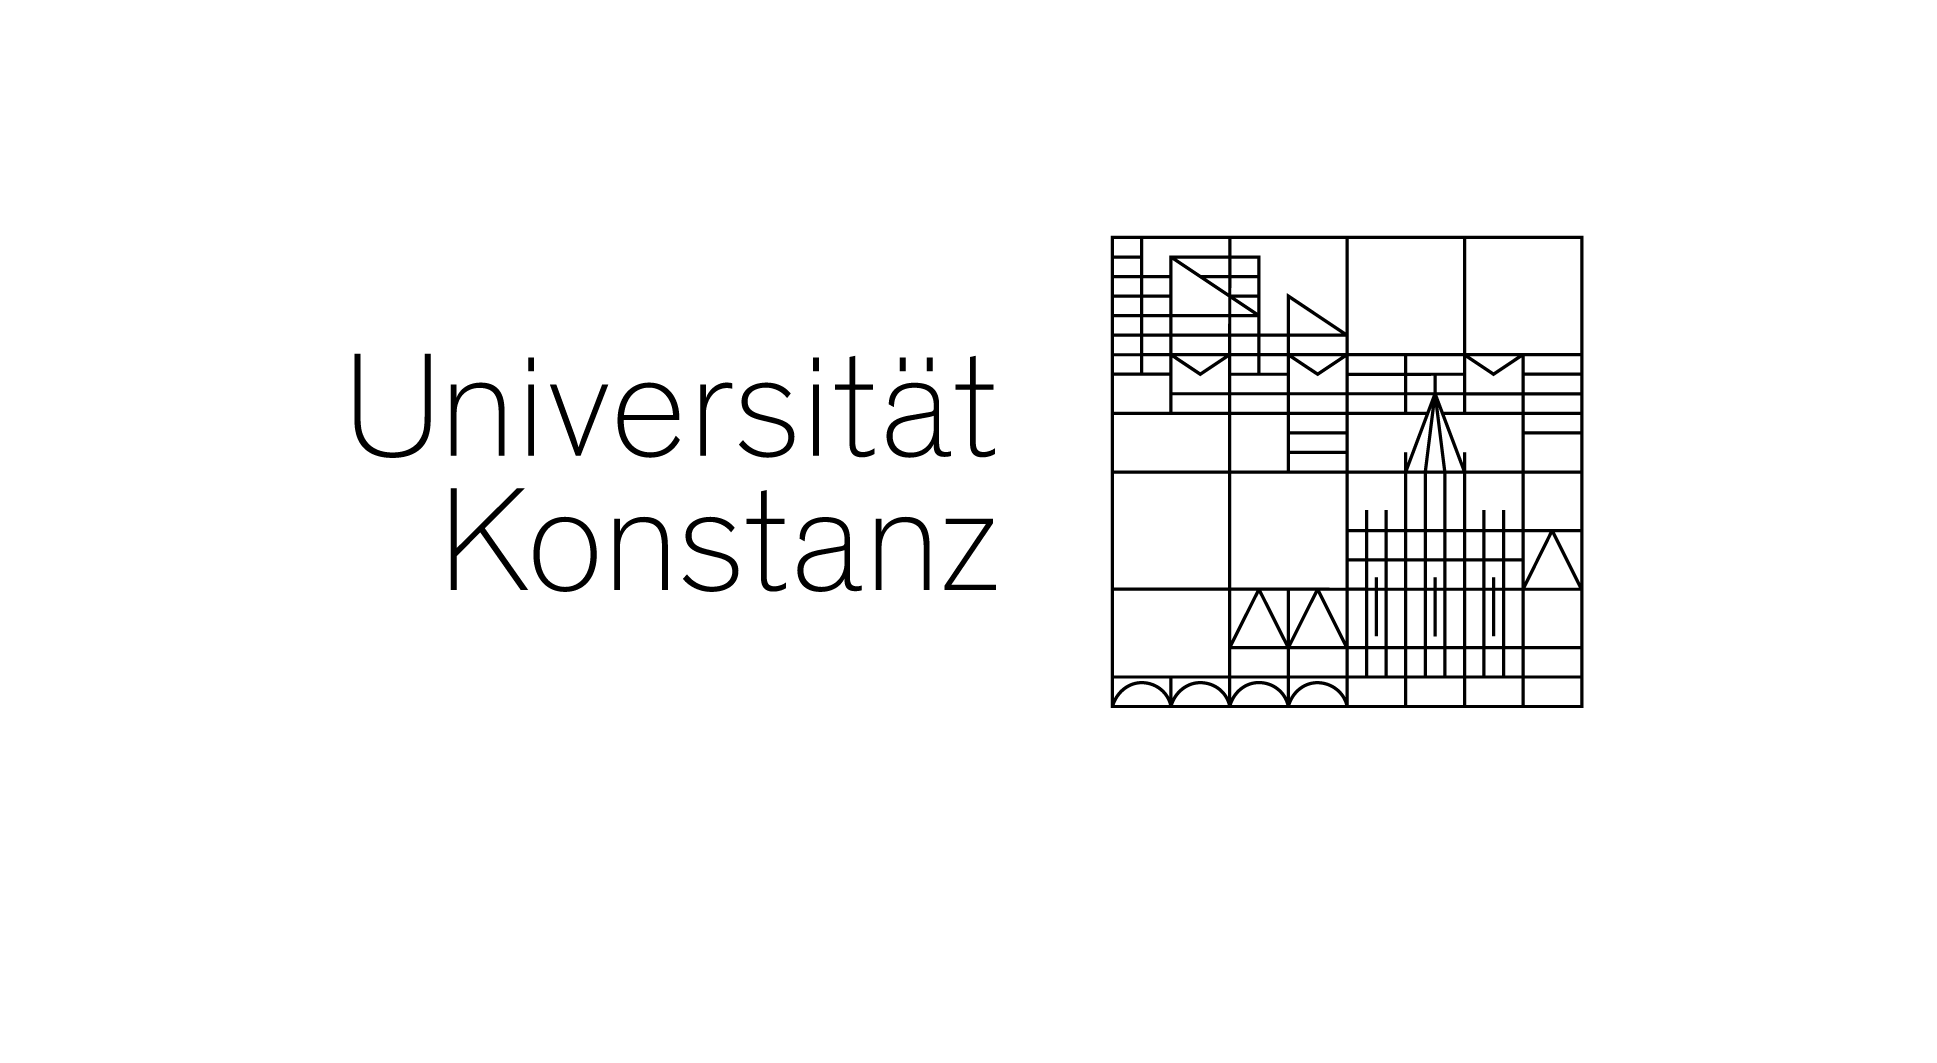
\includegraphics[width=1.2\textwidth]{logounikn} % first figure itself
				
			\end{minipage}\hfill
			\begin{minipage}{0.45\textwidth}
				\centering
				
\includegraphics[width=0.9\textwidth]{bsi_logo} % second figure itself
				
			\end{minipage}
		\end{figure}
		\centering
		\vspace{1cm}
		{\scshape\Large Universität Konstanz\\
			\large Fachbereich Mathematik und Statistik\\
			\& \\ \Large Bundesamt für Sicherheit in der Informationstechnik \par}
		\vspace{1cm}
		{\scshape\large Masterarbeit zum Thema:\par}
		\vspace{0.5cm}
		{\LARGE \bfseries Untersuchung \& Entwicklung von Ansätzen zur Detektion von Poisoning-Angriffen\par} %corher wars in \huge, das sah auch nicht so schlecht aus
		\vspace{0.5cm}
		\small vorgelegt von \par
		\vspace{0.5cm}
		{\large Lukas Schulth
			\par}
		%\vfill
		
		
		
		
		
		\vspace{1cm}
		\small unter der Betreuung von\par
		\centering
		\begin{figure}[h]
			\small
			\makebox[1 \textwidth][c]{   
				\begin{tabular}{ll}
					\pbox{20cm}{Erstgutachter: \\
						Herr Prof. Dr. Johannes Schropp \\ \texttt{johannes.schropp@uni.kn}} 
					& \pbox{20cm}{Zweitgutachter:\\
						Herr Prof. Dipl.-Ing. Markus Ullmann\\
						\texttt{markus.ullmann@bsi.bund.de}} \\ 
					&\\
					\pbox{20cm}{Herr Dr. Christian Berghoff \\ \texttt{christian.berghoff@bsi.bund.de}} 
					& \pbox{20cm}{Herr Matthias Neu \\ \texttt{matthias.neu@bsi.bund.de}}
					
				\end{tabular}
			}
		\end{figure}
		%\vfill
		%\vspace{0.25cm}
		% Bottom of the page
		{\large 1. Oktober 2021}
	\end{titlepage}
	
	
	
	%\selectlanguage{english}
	%\begin{abstract}english\end{abstract}
	%\selectlanguage{ngerman}
	%\begin{abstract}deutsch\end{abstract}
	
	%\keywords{one, two, three, four}
	\newpage
	%\thispagestyle{empty} 
	\listoffigures
	
	\listoftables
	
	%\lstlistoflistings
	
	\listofalgorithms
	\newpage
	\tableofcontents
	\newpage
	
	\chapter*{Abkürzungsverzeichnis}
	% https://www.heise.de/tipps-tricks/Abkuerzungsverzeichnis-in-LaTeX-erstellen-4982473.html
	\begin{acronym}[mAER]
		
		\acro{ac}[AC]{Activation-Clustering}
		\acro{aer}[AER]{Angriffserfolgsrate}
		\acro{cnn}[CNN]{Convolutional Neural Network}
		\acroplural{cnns}[CNNs]{Convolutional Neural Networks}
		\acro{acc}[ACC]{Genauigkeit}
		\acro{gwd}[GWD]{Gromov-Wasserstein-Distanz}
		\acro{hc}[HC]{Heatmap-Clustering}
		\acro{ki}[KI]{Künst\-li\-che In\-tel\-li\-genz}
		\acro{ki-genitiv}[KI]{Künst\-li\-chen In\-tel\-li\-genz}
		\acro{lkpa}[LkPA]{Label-konsistenter Poisoning-Angriff}
		\acro{lrp}[LRP]{Layer-wise Relevance Propagation}
		%\acro{ml}[ML]{Maschinelles Lernen}
		\acro{maer}[mAER]{mittlere Angriffserfolgsrate}
		\acro{nn}[NN]{Neuronales Netz}
		\acroplural{nn}[NNs]{Neuronale Netze}
		\acroplural{lkpa}[LkPAs]{Label-konsistente Poisoning-Angriffe}
		
		\acro{pa}[PA]{Poisoning-Angriff}
		\acroplural{pa}[PAs]{Poisoning-Angriffen}
		
		
		\acro{tnr}[TNR]{True Negative Rate}
		\acro{tpr}[TPR]{True Positive Rate}
		
		
		
	\end{acronym}
	%\printglossaries
	%\printglossary[type=\acronymtype]
	
	\chapter{Einführung}
	
	\begin{comment}
	
	Text and speech recognition, Maschinelle Übersetzung
	Image Recognition \footnote{\url{https://deepomatic.com/en/what-is-image-recognition}}
	

	Idee: \footnote{\url{https://arxiv.org/pdf/2007.08745v4.pdf}}
	Für einen Angriff auf ein Neuronales Netzwerk existieren mehrere Möglichkeiten.
	
	
	
	Definiere Adversariale Angriffe
	
	
	
	
	
	
	In poisoning attacks, attackers deliberately influence the
	training data to manipulate the results of a predictive model.
	
	\footnote{\url{https://ieeexplore.ieee.org/stamp/stamp.jsp?tp=&arnumber=8418594}}
	
	RIght to be forgottten,  General Data Protection Regulation (GDPR) in
	the European Union [5], \url{https://arxiv.org/pdf/2003.04247.pdf}, 5: G. D. P. Regulation, “Regulation (eu) 2016/679 of the
	european parliament and of the council of 27 april 2016
	on the protection of natural persons with regard to the
	processing of personal data and on the free movement
	of such data, and repealing directive 95/46,” Official
	Journal of the European Union (OJ), vol. 59, no. 1-88,
	p. 294, 2016.
	
	Datengewinnung(LRP)
	Datenverarbeitung(kMeans, Gromov Wasserstein)
	
	
	A Complete List of All (arXiv) Adversarial Example Papers \footnote{\url{https://nicholas.carlini.com/writing/2019/all-adversarial-example-papers.html}}
	\end{comment}
	
	Laut \cite{deeplearning_weather} befinden wir uns zurzeit in der dritten Hochphase der \ac*{ki-genitiv}\acused{ki}. Diese ist auch in Deutschland angekommen.	Es wird erwartet, dass mit Dienstleistungen und Produkten, die auf dem	Einsatz von \ac{ki} basieren, im Jahr 2025 Umsätze in Höhe von 488 Milliarden Euro generiert werden – damit würde ein Anteil von 13 Prozent am Bruttoinlandsprodukt erreicht werden. \\
	
	\noindent Unternehmen, die bisher keine Methoden des Maschinellen Lernens als Teil eines \ac{ki}-Systems verwenden, haben sich zumindest einmal die Frage gestellt, ob dadurch einzelne Arbeitsschritte erleichtert bzw. beschleunigt werden könnten und es damit zu einer Verbesserung der Produktivität kommen könnte. \\
	
	\noindent Obwohl die Wahrnehmung verbreitet ist, dass Maschinelles Lernen als Teil von \ac{ki} eine sehr neue Disziplin ist, reicht die zeitliche Entwicklung bis weit in das 20. Jahrhundert zurück. Das erste \ac{nn} wurde 1943 von McCulloch \& Pitts vorgestellt. Bis in die frühen 1960er Jahre war dies ein aktives Feld. Durch die Erfindung der Backpropagation erhielt das Maschinelle Lernen wieder große Aufmerksamkeit, da es nun möglich war, größere \acp{nn} zu konstruieren und trainieren, mit denen anschließend nicht-lineare Zusammenhänge in Daten gefunden werden konnten.\\
	\noindent Aufgrund fehlender Rechenleistung und wenig verfügbarer gelabelter Daten verlor das Maschinelle Lernen wieder an Aufmerksamkeit. Die dritte Welle der \ac{ki}, die bis heute anhält, geht auf drei bedeutende Entwicklungen um das Jahr 2010 zurück. Die Rechenkapazitäten vergößerten sich durch die Verwendung von Grafikkarten (GPUs) deutlich. Andererseits ermöglichte der Fokus auf \acp{cnn} die sehr effiziente Analyse riesiger (Bild-)Datensätze. Als Durchbruch gilt hier die Vorestellung von AlexNet \cite{alexnet} im Rahmen der ImageNet-Challenge \cite{imagenet}. Als dritter Punkt ist die Verfügbarkeit riesiger gelabelter Datensätze über das Internet zu nennen.\\
	%https://towardsdatascience.com/a-short-history-of-convolutional-neural-networks-7032e241c483
	
	
	\noindent Heute gibt es kaum noch einen Bereich, in dem Anwendungen auf Basis von \ac{ki} keine Rolle spielen, sei es in der Produktion, Werbung, Kommunikation, Biometrie oder Automotive. Viele Unternehmen nutzen \ac{ki}-Systeme, etwa um präzise Nachfrageprognosen anzustellen und das Kundenverhalten exakt vorherzusagen. Auf diese Weise lassen sich beispielsweise Logistikprozesse regional anpassen. Auch im Gesundheitswesen bedient man sich spezifischer \ac{ki}-Tätigkeiten wie dem Anfertigen von Prognosen auf Basis von strukturierten Daten. Hier betrifft das etwa die Bildverarbeitung: So werden Röntgenbilder als Input in ein \ac{ki}-System gegeben, der Output wird unterstützend für eine Diagnose verwendet. Das Erfassen von Bildinhalten ist auch beim autonomen Fahren entscheidend, wo Verkehrszeichen, Bäume, Fußgänger und Radfahrer fehlerfrei erkannt werden müssen. In solch sensiblen Anwendungsfeldern wie der medizinischen Diagnostik oder in sicherheitskritischen Bereichen müssen \ac{ki}-Systeme absolut zuverlässige Problemlösungsstrategien liefern \cite{fh1}.\\
	
	
	\noindent Dabei ist die Erklärbarkeit von Entscheidungen, die durch \ac{ki} getroffen werden, in
	sicherheitskritischen Anwendungsbranchen eine Voraussetzung für die Akzeptanz bei den Nutzern, für
	Zulassungs- und Zertifizierungsverfahren oder das Einhalten der durch die Datenschutzgrundverordnung (DSGVO) geforderten
	Transparenzpflichten \cite{kistudie}.
	
	\noindent Ein \ac{nn} als \ac{ki}-System kann als die Verkettung von linearen Funktionen und nicht-linearen Aktivierungsfunktionen verstanden werden.
	Zum Lebenszyklus eines \ac{ki}-Systems gehören die Datenerhebung und Datenaufbereitung, der Trainingsprozess, das Testen und die Inferenz, bei der das parametrisierte Netzwerk in der Anwendung genutzt wird. Häufig sind \acp{nn} klassischen Verfahren in ihrer Präzision deutlich überlegen, gleichzeitig fehlt es aber an der Interpretierbarkeit und damit an der Nachvollziehbarkeit getroffener Entscheidungen.
	
	\noindent Bei einem Entscheidungsbaum kann beispielsweise genau erklärt werden, aufgrund welcher Schwellenwerte welche Entscheidung zustande kommt. 
	Im Falle eines \ac{nn} liegen Millionen von Parametern vor, die genau verstanden und interpretiert werden müssen. \\
	
	\noindent Die Verwendung von immer größeren \acp{nn} mit Millionen von Parametern führte zu einem Durchbruch im Bereich der Bilderkennung (Klassifikation, Tagging, Segmentierung, Detektion, ...), welcher sich anschließend auf andere Bereiche wie beispielsweise Spracherkennung, Spiele oder Video-Analyse ausweitete.\\
	
	
	\noindent Es ist bekannt, dass die Präzision der \acp{nn} mit größeren Architekturen und größeren Datensätzen deutlich steigt. Um Rechenkapazitäten zu sparen, werden die Daten oft nicht selbst erhoben und gelabelt, sondern bereits verfügbare Datensätze übernommen. Zum Training der \acp{nn} werden oft Cloud-Computing-Plattformen verwendet, anstatt das \ac{nn} lokal zu trainieren oder es kommen vortrainierte \acp{nn} zum Einsatz, bei denen nur noch die letzten Schichten mit dem eigenen Datensatz trainiert werden müssen. All diese Schritte zur Einsparung von Ressourcen bedeuten gleichzeitig einen Verlust an Kontrolle, der von einem Angreifer ausgenutzt werden kann.\\
	
	\noindent Eine Möglichkeit sind sogenannte Adversariale Angriffe, die das vollständig trainierte \ac{nn} angreifen. Im Fall eines Klassifikationsproblems werden Datenpunkte so gestört, dass sie fälschlicherweise einer anderen Klasse zugeordnet werden. \\
	\acp{pa} finden im Gegensatz zu Adversarialen Angriffen vor bzw. während des Trainings statt. Dabei werden korrumpierte Daten in den Trainingsdatensatz eingeschleust, um die Vorhersagequalität eines \ac{nn} zu verringern.
	Das Ziel des Angreifers ist es, im Fall eines Klassifikationsproblems beispielsweise, die Präzision einer einzelnen Klasse zu verringern, während sich die Präzision auf allen anderen Klassen gar nicht oder nur leicht verändert.\\
	Ein Spezialfall sind die sogenannten Backdoor-Poisoning-Angriffe, bei denen der Angreifer eine Art Hintertür im Datensatz implementiert, die während der Inferenz ausgenutzt werden kann. Damit erfolgt eine aus Sicht des Angreifers gewollte falsche Klassifikation nur dann, wenn dem \ac{nn} eine Eingabe präsentiert wird, die einen solchen Auslöser enthält.\\
	Diese Angriffe können in ihrer Detektion noch zusätzlich erschwert werden, indem das entsprechende Label nicht abgeändert wird. In diesem Fall sprechen wir von Label-konsistenten Poisoning-Angriffen. \\
	 
	
	\noindent Es ist noch immer schwierig, die konzeptionell leicht umzusetzenden \acp{pa} erfolgreich zu detektieren.
	Die Detektion von \acp{pa} erweist sich grundsätzlich als schwierig, vor allem deshalb, weil sich das \ac{nn} nur in der Präsenz eines Auslösers anders verhält.	\\
	
	\noindent Die in dieser Arbeit untersuchte Idee für ein verbessertes Verfahren zur Detektion von Poisoning-Angriffen liefert \cite{unmaskingCH}. 
	Dort werden Datensätze auf sogenannte Clever Hans-Artefakte (CH-Artefakte) untersucht. Ein CH-Artefakt bezeichnet ein Merkmal einer Netzeingabe einer bestimmten Klasse, die zur selben, richtigen Entscheidung des \ac{nn} führt, der Grund dafür jedoch abweichend ist. D.h. für eine Eingabe mit einem CH-Artefakt besitzt das \ac{nn} eine andere Entscheidungsstrategie. Eine Möglichkeit, solche unterschiedlichen Strategien zu quantifizieren bietet die Methode \ac{lrp}, die einzelnen Bereichen einer Eingabe bestimmte Relevanzen bezüglich einer getroffenen Entscheidung zuordnet. Die \ac{lrp} gehört zu den lokalen Verfahren der Erklärbaren Künstlichen Intelligenz, die Erklärungen für einzelne Netzentscheidungen liefern können. Basierend darauf wollen wir ein Clustering-Verfahren anwenden, um \acp{pa} zu detektieren. Anschließend vergleichen wir dieses Vorgehen mit dem sogenannten \ac{ac}, mit dem ebenfalls \acp{pa} detektiert werden können. \\
	
	
	\noindent Die vorliegende Arbeit ist wie folgt strukturiert: In \autoref{chapter1} stellen wir die theoretischen Grundlagen vor, die für Angriffe und die Detektion von \acp{pa} notwendig sind. In \autoref{chapter_nn} geben wir eine kurze Einführung in \acp{nn} und stellen den klassischen Trainingsprozess vor. \autoref{chapter_poisoningattacks} führt in die unterschiedlichen Möglichkeiten eines \ac{pa} auf \ac{nn} ein. \autoref{chapter_xai} gibt eine kurze Übersicht über den Bereich der Erklärbaren Künstlichen Intelligenz, wobei ein Beispiel eines Verfahrens, die sogenannte Layer-wise Relevanz Propagation ausführlich in \autoref{chapter_lrp} vorgestellt wird. Den Kern dieser Arbeit bildet \autoref{chapter:algorithm}, wo wir zu Beginn die grundlegenden Bestandteile des Algorithmus zur Detektion von \acp{pa} auf \acp{nn} erklären. In \autoref{chapter_results} stellen wir das verwendete Netz, den Datensatz, die ausgeführten Angriffe und Verteidigungen vor und vergleichen die einzelnen Verfahren miteinander.
	In \autoref{chapter_conclusion} geben wir eine Zusammenfassung und blicken auf mögliche weitere Untersuchungen.
	
	
	
	
	
	
	
	
	
	
	
	
	

	

	\chapter{Theoretische Grundlagen}\label{chapter1}
	
	\section{Theorie des Optimalen Transports}\label{ot}
	\begin{comment}
	
	Optimal Transport is an interesting topic which connects many fields and has
	interesting applications
	Applications in image analysis
	Interplay between geometry, probability and PDEs
	Convexity, duality
	Numerical optimization
	Statistics and Machine Learning\footnote{\url{https://indico.cern.ch/event/845380/attachments/1915103/3241592/Dvurechensky_lectures.pdf}}
	
	Optimal transport can deal with smooth and discrete measures and it has proved to be very useful
	for comparing distributions in a shared space, but with different (and even non-overlapping) supports\cite{vayer2020fused}.
	Einführung OT Villani%\footnote{\url{https://books.google.de/books?hl=en&lr=&id=idyFAwAAQBAJ&oi=fnd&pg=PR11&dq=villani+2003&ots=YRvDCQXIIn&sig=XqyOf4Qqsw-otlBm0_4L3YoU6pA&redir_esc=y#v=onepage&q=villani\%202003&f=false}}
	OT hebt Distanzen von metrischen Räumen auf den Raum der metrischen Räume \cite{memoli2011gromov}.
	content...
	\end{comment}
	
	In diesem Kapitel betrachten wir einige Konzepte aus dem Bereich des Optimalen Transports, um einen Distanzbegriff zu entwickeln, der im Unterschied zur pixelweisen euklidischen Distanz besser für das $k$Means-Clustering (vgl. \autoref{chapter:kMeans}) geeignet sein könnte.
	Ausgehend von Gaspard Monge's ursprünglicher Trans\-port\-pro\-blem-For\-mu\-lie\-rung betrachten wir die durch Kantorovich vorgestellte Relaxierung dieses Problems.
	Die Lösung des Optimierungsproblems wird für die Definition der $p$-Wasserstein-Distanz verwendet. Damit wird ein Distanzbegriff zwischen einzelnen Punkten auf einen Distanzbegriff zwischen Wahrscheinlichkeitsmaßen übertragen.
	Für eine Verallgemeinerung auf verschiedene Grundräume wird die \ac{gwd} definiert. Damit können wir zwei Heatmaps als sogenannte metrische Maßräume auffassen und eine Distanz zwischen diesen berechnen.
	Abschließend definieren wir sogenannte Gromov-Wasserstein-Baryzentren, die im Rahmen des $k$Means-Clustering als Mittelwerte fungieren.
	
	\noindent Wir beschäftigen uns im Folgenden ausschließlich mit diskreten Wahrscheinlichkeitsverteilungen. Grundlegend dafür sind die folgenden Definitionen.
	\subsection{Grundbegriffe der Maßtheorie}
	In diesem Abschnitt stellen wir ganz kurz die aus der Maß- und Wahrscheinlichkeitstheorie wichtigen Begriffe vor, die wir im Folgenden für die Konstruktion der Wasserstein- und  Gromov-Wasserstein-Distanz benötigen.
	\begin{comment}
	
	Was ist ein registration problem?
	Warum brauchen wir Gromov-Wasserstein? Warum reicht nicht Wasserstein? Weil wir Matrizen unterschiedlicher Größer vergleichen? Nein. Wir benutzen ja immer dieselbe Distanz für alle Pixel-Werte.
	Wenn wir eine Pixel-Wolke auswählen, sind das nicht dieselben Räume, da dann gewisse Koordinaten nicht zum Raum gehören. Wenn wir aber alle Pixel als Koordinaten im Raum auswählen würden, dann würden die metrischen Räume $(X,d_X)$ und $(Y,d_Y)$ übereinstimmen. Liegt das an der Definition der Baryzentren? Wie würde man das mit Baryzentren auf demselben Raum machen? s. \cite{COTcuturi}
	Translationen und Rotationen könnte ein wichtiger Punkt sein!!!
	verwendung von Grafiken aus anderen Papern??
	Kann man ein anderes Netzwerk zur Detektion nutzen?
	
	\url{https://arxiv.org/pdf/1705.09634.pdf}
	\url{https://arxiv.org/pdf/1412.5154.pdf}
	Für die Grudnlagen im Bereich des Optimalen Transports zitieren wir \cite villani2009optimal.
	
	Entscheidend für die Numerischen Resultate ist die Arbeit von Marco Cuturi \cite{cuturi2013sinkhorn, computationalOT}
	
	\cite{COTcuturi} Remark 2.19 (Translations). zeigt dass die Unabhängigkeit gegenüber Translationen? Kann ich das auch für die Gromov-Wasserstein-Distanz zeigen?
	
	Optimal transport is also used widely in domain adaptation \cite{courty2016optimal}. In domain adaptation, one has
	access to labeled examples from a source domain and unlabeled examples from a target domain.
	The goal is to predict labels for examples from the target domain. This is different from the typical
	train-test paradigm in machine learning, because covariate shift between the two domains is allowed.
	
	
	Ein weitere Anwendung von Optimal Transport sind Wasserstein Generative Adversarial Networks (WGANs) \cite{wgan}. WGANs gehören zur Familie der Modelle namens Generative Adversarial Networks (GANs) \cite{gan}. Zu einem GAN gehören zwei Modelle, von denen beide typischerweise Neuronale Netzwerke sind. Das erste Netzwerk (generator) erzeugt Datenpunkte innerhalb des Datensatzes, die so realsitisch wie möglich sein sollen. Das zweite Netzwerk (discriminator network) versucht, zwischen den realen und den erzeugten Datenpunkten zu unterscheiden. Damit kann der Trainingsprozess von GANs als ein Spiel zwischen den beiden Netzwerken betrachtet werden, bei dem der Generator den Diskriminator täuschen und der Diskriminator die korrumpierten Datenpunkte aufdecken möchte.
	
	Durch die Verwendung von WGANs ansatts GANs wurde ein stabilerer Trainingsprozess erreicht, da diese weniger anfällig für abrupte Trainingsabbrüche sind. Die ursprünglichen GANs benutzten eine Jensen-Shannon-Divergenz als Verlustfunktion, die nicht überall stetig und fast überall differenzierbar ist. Auch andere Verlustfunktion wie besipielsweise die KL-Divergenz weisen ähnliche Schwierigkeiten auf. Durch die Verwendung der Wasserstein-Verlustfunktion, basierend auf der 1-Wasserstein-Distanz, die überall stetig und fast überall differenzierbar ist, konnte der Trainingsprozess der GANs somit deutlich verbessert werden \cite{mauryaoptimal}.
	
	\end{comment}
	
	\begin{definition}\cite{burago2001course}
		Sei $X$ eine beliebige Menge. Eine Funktion $d:X \times X \to \mathbb{R} \cup \lbrace \infty \rbrace$ heißt \emph{Metrik} auf $X$, falls die folgenden Bedingungen für alle $x,y,z \in X$ gelten:
		\begin{enumerate}[label={(\arabic*)}]
			\item Positive Definitheit: $d(x,y) > 0 \text{ für } x \neq y \text{ und } d(x,y)=0 \text{ für } x=y$,
			\item Symmetrie: $d(x,y)=d(y,x)$,
			\item Dreiecksungleichung: $d(x,z) \leq d(x,y) + d(y,z)$.	
		\end{enumerate}
	\end{definition}
	\noindent Ein \emph{metrischer Raum} ist eine Menge, versehen mit einer Metrik. Formal gesehen ist ein metrischer Raum ein Paar $(X,d)$, wobei $d$ eine Metrik auf $X$ ist. Elemente von $X$ heißen Punkte und $d(x,y)$ bezeichnet die Distanz zwischen $x$ und $y$.
	
	
	\begin{definition}\cite{COTcuturi}
		Als Histogramm (oder: Zufallsvektor) bezeichnen wir ein Element $\boldsymbol{a} \in \Sigma_n$, das zum folgenden Wahrscheinlichkeits-Simplex gehört:
		
		\begin{equation*}
		\Sigma_n := \lbrace \boldsymbol{a} \in \mathbb{R}_{+}^n | \sum_{i=1}^n{\boldsymbol{a_i} = 1} \rbrace
		\end{equation*}
	\end{definition}
	
	\begin{definition}\cite{COTcuturi}
		Ein diskretes Maß mit Gewichtung $\boldsymbol{a}$ und Punkten $x_1,...,x_n \in X$ wird geschrieben als
		\begin{equation}
		\alpha = \sum_{i=1}^n{\boldsymbol{a}_i\delta_{x_i}},
		\end{equation}
		wobei $\delta_x$ das Dirac-Maß an Position $x$ ist. Gilt $\boldsymbol{a} \in \Sigma_n$ und $\boldsymbol{a}_i >0$ f.a. $i$, so sprechen wir von einem diskreten Wahrscheinlichkeitsmaß.
	\end{definition}
	
	\begin{definition}\cite{gromov2007metric}\\
	%TODO: Absetzen:remark
		Ein \emph{metrischer Maßraum} ist ein Tripel $(X,d_X,\mu_X)$ mit
		\begin{itemize}
			\item $(X, d_X)$ ist ein kompakter metrischer Raum
			\item $\mu_X$ ist ein Borel-Maß auf $X$ mit vollem Support, d.h. 
			\begin{equation}
			supp[\mu_X] = X.\label{eq:bed_mmspaces}
			\end{equation} 
		\end{itemize}
	\end{definition}
	
	\begin{definition}[Isometrie]
		Seien zwei metrische Räume $(X, d_X)$ und $(Y,d_Y)$ gegeben. Wir nennen die Abbildung $\phi:X \to Y$ Isometrie, falls $\phi$ surjektiv ist und $d_X(x,x')= d_Y(\phi(x),\phi(x'))$ f.a. $x, x' \in X$ gilt. \\
		\noindent Falls eine solche Abbildung $\phi$ existiert, nennen wir $X$ und $Y$ isometrisch.
	\end{definition}
	
	\begin{definition}[Bildmaß]
		Seien $X,Y$ zwei Maßräume, $T: X \to Y$ eine messbare Abbildung und $\mu$ ein Maß auf X. Dann ist das Bildmaß (oder: pushforwad-Maß) $T^\# \mu $ ein Maß auf Y, definiert durch \begin{equation}
		T^\# \mu (A) = \mu (T^{-1}(A))
		\end{equation}
		für alle $A \subset Y$.
	\end{definition}
	
	%\begin{definition}[Bildmaß]
	%	Für zwei Maßräume $(X,\Sigma_X)$ und $(Y,\Sigma_Y)$ und eine messbare Abbildung $f:X\to Y$ ist das Bildmaß $f_\#\mu$ auf $(Y,\Sigma_Y)$ definiert als $f_\#\mu = \mu (f^{-1(B)})$ für alle $B \in \Sigma_Y$.
	%\end{definition}
	
	\begin{definition}[Isomorphie]
		Zwei metrische Maßräume $(X,d_X,\mu_X)$ und $(Y,d_Y,\mu_Y)$ heißen isomorph, falls eine Maß-erhaltende Abbildung $f:X \to Y$ existiert, die $f_\#\mu_X = \mu_Y$ erfüllt.
	\end{definition}
	
	\noindent Mit $\mathcal{G}_\mathcal{W}$ bezeichnen wir die Menge aller metrischen Maßräume.
	
	\begin{example}
		Wir betrachten die beiden metrischen Maßräume 
		\begin{equation}
		\left( \lbrace a,b \rbrace, \begin{pmatrix}
		0 & 1\\
		1 & 0 \\
		\end{pmatrix}, \lbrace \frac{1}{2},\frac{1}{2} \rbrace \right) \text{ und } 
		\left(\lbrace a',b' \rbrace, 
		\begin{pmatrix}
		0 & 1\\
		1 & 0 \\
		\end{pmatrix}, \lbrace \frac{1}{4},\frac{3}{4}\rbrace \right).
		\end{equation}
		\noindent Dann sind diese Räume isometrisch, jedoch nicht isomorph, siehe \autoref{im:example_mmspaces}.
	\end{example}
	
	\begin{figure}[ht]
		\centering
		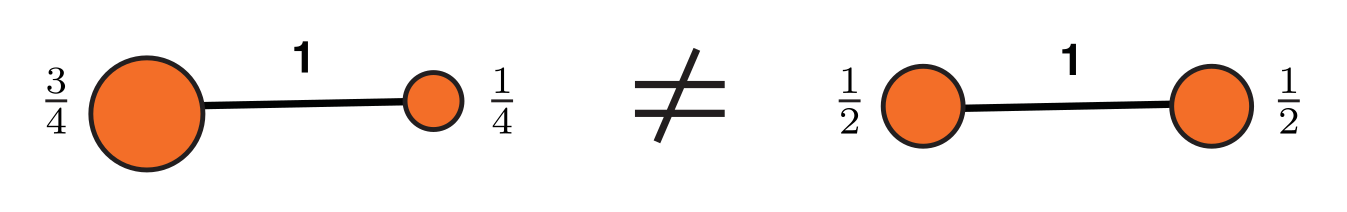
\includegraphics[width=0.3\textheight]{example_mmspaces.png}
		\caption[Beispiel isometrischer metrischer Maßräume]{Die beiden metrischen Maßräume sind isometrisch, aber nicht isomorph.}
		\source{\cite{COTcuturi}}
		\label{im:example_mmspaces}
	\end{figure}
	
	\begin{comment}
		\begin{definition}[Kopplung]
		Ein Wahrscheinlichkeitsmaß $\mu$ auf $X \times Y$ heißt Kopplung zwischen $\mu_x$ und $\mu_Y$, falls $(\mu_1)_\#\mu = \mu_X$ und $(\mu_2)_\#\mu = \mu_Y$ gilt. Wir benzeichnen mit $\Pi(\mu_X,\mu_Y)$ die Menge aller Kopplungen ziwschen $\mu_X$ und $\mu_Y$.
		\end{definition}
	\end{comment}
	
	
	
	%Einführung W-Theorie am KIT \footnote{\url{https://www.math.kit.edu/stoch/~henze/media/wt-ss15-henze-handout.pdf}}
	
	\begin{comment}
		\begin{definition}[Kopplungen zwischen Histogrammen]
		Seien die beiden Histogramme $p \in \Sigma_{N_1}$ und $q \in \Sigma_{N_2}$ gegeben.
		Als Menge der Kopplungen zwischen beiden Histogrammen definieren wir
		
		\begin{equation*}
		\Pi (p,q) := \lbrace T \in (\mathbb{R}_+)^{N_1 \times N_2} | T \boldsymbol{1}_{N_2} = p, T^\top \boldsymbol{1}_{n_1} = q \rbrace,
		\end{equation*}	
		
		\noindent wobei $\boldsymbol{1}_N := (1,...,1)^\top \in \mathbb{R}^{N}$ gilt.
		\end{definition}
	\end{comment}
	
	
	
	
	
	
	
	
	
	%Geodesic Space \footnote{\url{http://www.math.toronto.edu/mccann/papers/FiveLectures.pdf}}
	
	
	
	
	
	
	
	
	
	
	%\subsection{Notation}
	%siehe: Introduction to Optimal Transport
	%Matthew Thorpe
	
	%\url{http://inis.jinr.ru/sl/vol2/Ax-books/Disk_01/Gromov-Metric-structures-Riemann-non-Riemann-spaces.pdf}
	\subsection{Optimaler Transport nach Kantorovich}
	In diesem Abschnitt wollen wir einen Ähnlichkeitsbegriff für Maße einführen. Der Bereich des Optimalen Transports beschäftigt sich mit der Frage, wie mehrere Objekte, die sich in einer bestimmten Verteilung an einem Startpunkt befinden, auf optimale Weise zu einem Zielpunkt transportiert werden können. Dabei wird die Verteilung der Objekte als Wahrscheinlichkeitsverteilung interpretiert. 
	
	
	\subsubsection{Optimaler Transport (Formulierung von Monge)}
	
	Dieses Problem wurde zuerst von Gaspard Monge im Jahr 1781 formuliert. In dieser Formulierung wird eine Abbildung gesucht, die jedem Punkt in der Ausgangsverteilung einen Punkt in der Zielverteilung zuordnet. Dabei wird die gesamte Masse eines Punktes in der Startverteilung auf einen Punkt in der Zielverteilung verschoben. Eine solche Abbildung ist in \autoref{im:monge_mapping} dargestellt.
	
	\begin{figure}[ht]
		\centering
		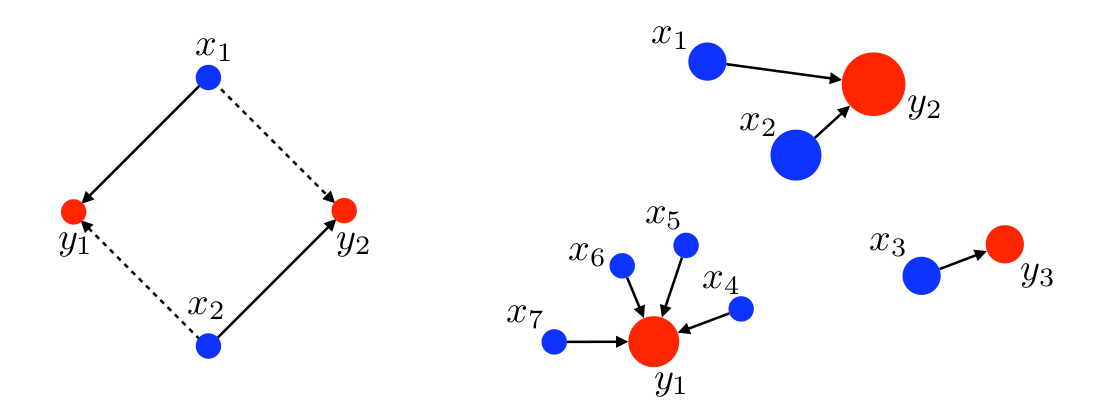
\includegraphics[width=0.3\textheight]{monge_mapping.png}
		\caption[Monge-Abbildung]{\textbf{Links:} Fehlende Eindeutigkeit in der Zuordnung. Die beiden Punkte $x_1$ und $x_2$ können sowohl den Punkten $y_1$ bzw. $y_2$ zugeordnet werden, um eine zulässige Abbildung zu erhalten. \textbf{Rechts:} Die Monge-Abbildung assoziiert das blaue Maße $\boldsymbol{\alpha}$ mit dem roten Maß $\boldsymbol{\beta}$. Dabei ist die Masse in den jeweiligen Punkten über den Flächeninhalt der Kreise dargestellt.}
		\source{\cite{COTcuturi}}
		\label{im:monge_mapping}
	\end{figure}
	
	
	
	
	
	\noindent Für den Fall zweier diskreter Maße
	
	\begin{equation}
	\alpha = \sum_{i=1}^n{\boldsymbol{a}_i\delta_{x_i}} \text{ und } \beta = \sum_{j=1}^m{\boldsymbol{b}_j\delta_{y_j}}
	\end{equation}
	können wir das Monge-Problem  wie folgt formulieren:
	
	\noindent Gesucht ist eine Abbildung $T:\lbrace x_1, ..., x_n \rbrace \to \lbrace y_1,...,y_m \rbrace$, die die Bedingung 
	\begin{equation}
	\forall j \in \lbrace 1,...,m \rbrace: \quad \boldsymbol{b}_j= \sum_{i:T(x_i)=y_i}{\boldsymbol{a}_i}
	\end{equation}
	erfüllt, die wir in Kurzform als $T_\#\alpha = \beta$ schreiben. Aufgrund der Positivität von $\boldsymbol{b}$ ist die Abbildung notwendigerweise surjektiv.
	Als weitere Forderung gilt, dass die Abbildung $T$ minimal bezüglich einer Transportkostenfunktion $c(x,y)$ für $(x,y) \in \mathbb{R} \times \mathbb{R}$ sein soll:
	\begin{equation}
	T = \min_S{\Big\{ \sum_i{c(x_i, S(x_i)) : S_\#\alpha =  \beta} \Big\}}.
	\end{equation} 
	
	\noindent Neben der fehlenden Eindeutigkeit einer solchen Abbildung ist auch die Existenz nicht immer gegeben. Eine Lösung dafür liefert die Formulierung von Kantorovich im folgenen Abschnitt.
	
	\subsubsection{Optimaler Transport nach Kantorovich}
	%\cite{santambrogio2010introduction} ist eine gute, einfache Einführung. Damit kann ich vermutlich Monge und Kantorovich beschreiben.
	
	Das Problem des Optimalen Transports nach Kantorovich gehört zu den typischen Optimal Transport Problemen. Es stellt eine Relaxierung der Formulierung von Gaspard Monge dar, bei der nun auch das Aufteilen von Masse (mass splitting) zulässig ist, d.h. die Masse an einem Startpunkt kann auf mehrere Zielpunkte abgebildet werden.\\
	
	\noindent In Kantorovichs Formulierung ist eine Kopplung (oder: Transportabbildung/ Transportplan) $\boldsymbol{P} = (\boldsymbol{P}_{i,j})_{i,j} \in \mathbb{R}^{n\times m}$ gesucht, die die Kosten, die bei der Verschiebung eines diskreten Maßes $\boldsymbol{a}$ auf ein anderes diskretes Maß $\boldsymbol{b}$ bezüglich der Kosten $\boldsymbol{C} = (\boldsymbol{C}_{i,j})_{i,j} \in \mathbb{R}^{n \times m}$ entstehen, minimiert. Die Einträge $\boldsymbol{P}_{i,j}$ geben an, wie viel der Masse von $x_i$ nach $y_j$ transportiert werden soll. Die Einträge $\boldsymbol{C}_{i,j}$ beschreiben die Kosten, um eine Einheit von $x_i$ nach $y_j$ zu transportieren.  \\
	
	\noindent Damit $\boldsymbol{P}$ eine Transportabbildung ist, muss $\boldsymbol{P} \in \Pi(a,b) = \lbrace \boldsymbol{P} \geq \boldsymbol{0}, \boldsymbol{P}\boldsymbol{1}_{m} = \boldsymbol{a}, \boldsymbol{P}^\top\boldsymbol{1}_{n} = \boldsymbol{b} \rbrace$ gelten. Dabei bedeutet die erste Forderung, dass nur positive Anteile verschoben werden können. Die beiden letzten Bedingungen fordern, dass die gesamte verschobene Masse der Start- bzw. Zielverteilung entspricht und somit keine Masse entsteht oder verloren geht.
	
	\noindent Ein großer Vorteil des Optimalen Transports ist, dass neben dem Vergleich von diskreten mit diskreten und stetigen mit stetigen Verteilungen auch der Vergleich von diskreten und stetigen Verteilungen miteinander möglich ist. Transportpläne für diese drei verschiedenen Problemstellungen sind in \autoref{im:couplings} dargestellt.
	
	\begin{figure}[ht]
		\centering
		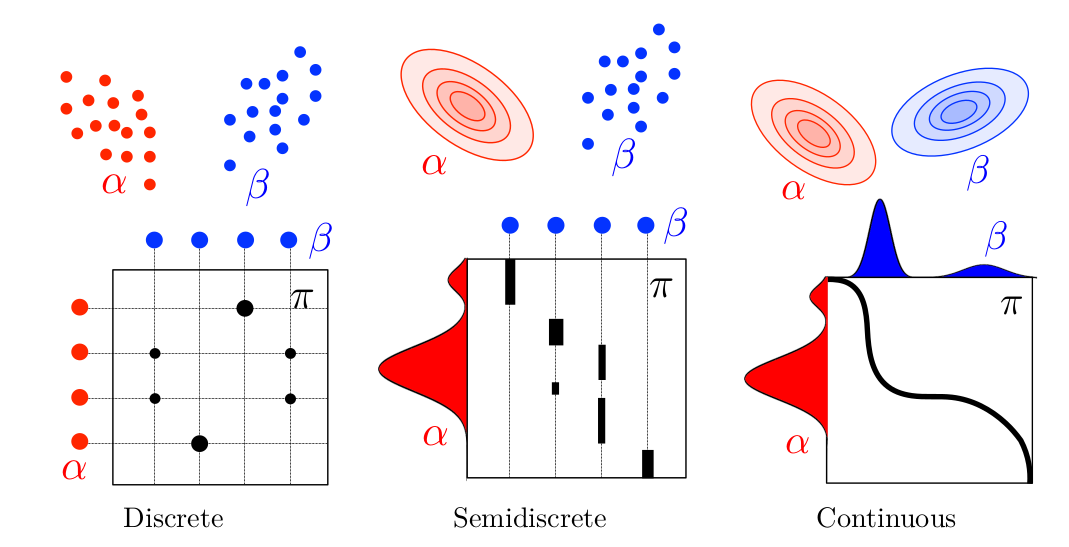
\includegraphics[width=0.4\textheight]{coupling_disc_semid_cont.png}
		\caption[Transportpläne im diskreten, semi-diskreten und kontinuierlichen Fall]{\textbf{Links: }Kopplung zwischen zwei diskreten Wahrscheinlichkeitsverteilungen. \textbf{ Mitte: }Kopplung zwischen einer kontinuierlichen Wahrscheinlichkeitsverteilung $\boldsymbol{\alpha}$ und einer diskreten Wahrscheinlichkeitsverteilung $\boldsymbol{\beta}$. \textbf{Rechts: }Kopplung im kontinuierlichen Fall.}
		\source{\cite{COTcuturi}}
		\label{im:couplings}
	\end{figure}
	
	
	\noindent Gesucht ist nun auch hier der optimale Transportplan, der die entstehenden Gesamtkosten minimiert. 
	\begin{comment}
		
	
	Das OT Problem ist definiert als
	\begin{equation}
	W_M(\boldsymbol{a},\boldsymbol{b}) = \min_{P \in \Pi(\boldsymbol{a}, \boldsymbol{b})}{\langle \boldsymbol{P}, \boldsymbol{M} \rangle},
	\end{equation}
	
	wobei ${\langle \boldsymbol{P}, \boldsymbol{M} \rangle} = \sum_{ij}{t_{ij}m_{ij}}$ gilt.
	
	Die Lösung des Problems ist eine Kopplung/Kopplungsmatrix, die beschreibt, wie viel Masse von einem Punkt zum anderen Punkt fließt. In einer Kostenmatrix derselben Größe sind die Kosten abgespeichert, um von einem zum anderen Punkt zu kommen.
	
	Die Menge der Matrizen $\Pi(\boldsymbol{a}, \boldsymbol{b})$ ist beschränkt und durch $n+m$ Gleichungen gegeben und damit ein konvexes Polytop (die konvexe Hülle einer endlichen Menge von Matrizen). Zudem ist die Formulierung von Kantorovich im Unterschied zu Monges Formulierung immer symmetrisch in dem Sinne, dass $\boldsymbol{P} \in \Pi (\boldsymbol{a}, \boldsymbol{b})$ genau dann gilt, wenn $\boldsymbol{P}^\top \in \Pi (\boldsymbol{b}, \boldsymbol{a})$.
	\end{comment}
	Kantorovichs Optimal Transport Problem lässt sich nun schreiben als 
	\begin{equation}
	L_C(\boldsymbol{a}, \boldsymbol{b}) := \min_{P \in \Pi(\boldsymbol{a}, \boldsymbol{b})} \langle \boldsymbol{C}, \boldsymbol{P} \rangle := \min_{P \in \Pi(\boldsymbol{a}, \boldsymbol{b})} \sum_{i,j}{\boldsymbol{C}_{i,j}\boldsymbol{P}_{i,j}} \label{KOTP}
	\end{equation}
	
	\noindent Dies ist ein lineares Problem, dessen Lösung nicht notwendigerweise eindeutig ist. Kantorovich gilt als Erfinder der linearen Optimierung \cite{intro_ot_thorpe}.
	\begin{comment}
	
	Im Fall beliebiger Maßer egibt sich die folgende
	
	\begin{definition}[Formulierung für beliebige Maße]
	Im Fall beliebiger Maße betrachten wir die Kopplungen $\pi \in \mathcal{M}_+^1(\mathcal{X} \times \mathcal{Y})$, die die gemeinsame Verteilung auf dem Produktraum $\mathcal{X} \times \mathcal{Y}$ ist. Im diskreten Fall verlangen wir, dass das Produktmaß die Form $ \pi = \sum_{i,j}{\boldsymbol{P}_{i,j}\delta_{(x_i, y_j)}}$ besitzt. Im Allgemeinen Fall wird die Massenerhaltung als Randbedingung an die gemeinsame W-Verteilung geschrieben:
	
	\begin{equation}
	\Pi(\alpha, \beta) := \lbrace \pi \in \mathcal{M}_+^1(\mathcal{X} \times \mathcal{Y}): P_{\mathcal{X}_\#} \pi = \alpha \text{ und } P_{\mathcal{Y}_\#} \pi = \beta \rbrace,
	\end{equation}
	wobei $P_{\mathcal{X}_\#}$ und $P_{\mathcal{Y}_\#}$ die Bildmaße der Projektionen $P_\mathcal{X}(x,y) = x$ und $P_\mathcal{Y}(x,y) = y$ sind. Nach \autoref{eq_pushforward} sind diese Randbedingungen äquivalent zu den Bedingungen $\pi(A \times \mathcal{Y}) = \alpha (A)$ und $\pi (\mathcal{X} \times B) = \beta (B)$ für die Mengen $A \subset \mathcal{X}$ und $B \subset \mathcal{Y}$.
	Als Verallgemeinerung erhalten wir dann
	\begin{equation}
	\min_{\pi \in \Pi (\alpha, \beta)}\int_{\mathcal{X} \times \mathcal{Y}}{c(x,y) d\pi (x,y)}. \label{eq:kontorovich_allgemein}
	\end{equation}
	\end{definition}
	
	\end{comment}
	\begin{comment}
		Problem \autoref{KOTP} ist ein unendlich-dimensionales lineares Optinmierungsproblem über einem Raum von Maßen. Falls $(\mathcal{X}, \mathcal{Y})$ kompakt und $c$ stetig ist, existiert immer eine Lösung.
	\end{comment}

	
	
	\subsubsection{Metrische Eigenschaften}
	Für den Fall, dass die Grundkosten eine Metrik darstellen, ist auch die optimale Lösung des Optimal Transport Problems wieder eine Metrik \cite{cuturi2014ground} und definiert die Wasserstein-Distanz wie folgt:
	
	
	\begin{definition}[p-Wasserstein-Distanz auf $\Sigma_n$]
		Sei $n=m$ und für $p \geq 1$ gelte $\boldsymbol{C} = \boldsymbol{D}^p = (\boldsymbol{D}_{i,j}^p)_{i,j} \in \mathbb{R}^{n \times n}$, wobei $\boldsymbol{D} \in \mathbb{R}_+^{n \times n}$ eine Metrik ist.
		
		\noindent Dann definiert 
		\begin{equation}
		W_p(\boldsymbol{a}, \boldsymbol{b}) := L_{\boldsymbol{D}^p} (\boldsymbol{a}, \boldsymbol{b})^{1/p}
		\end{equation} 
		die $p$-Wasserstein-Distanz auf $\Sigma_n$
	\end{definition}
	
	\begin{lemma}\cite{COTcuturi, villani2003topics}
		$W_p$ ist eine Metrik
	\end{lemma}
	
	\begin{proof}
		Nach Voraussetzung besitzt $\boldsymbol{C} = \boldsymbol{D}^p$ eine Nulldiagonale. Somit gilt $W_p(\boldsymbol{a},\boldsymbol{a}) =0.$. Die zugehörige Transportmatrix ist $\boldsymbol{P}^\star = diag(\boldsymbol{a})$. Aufgrund der Positivität aller Nicht-Diagonalelemente von $\boldsymbol{D}^p$ gilt $W(\boldsymbol{a},\boldsymbol{b}) > 0 $ für $\boldsymbol{a} \neq \boldsymbol{b}$, da in disem Fall jede zulässige Kopplung und damit insbesondere die optimale Kopplung ein Nicht-Diagonalelemnt ungleich $0$ besitzt. Die Symmetrie von $W_p(\boldsymbol{a},\boldsymbol{b})$ gilt wegen der Symmetrie von $\boldsymbol{D}^p$.\\
		
		\noindent Für den Nachweis der Dreiecksungleichung im Fall beliebiger Maße nutzt Villani \cite{villani2003topics} das sogenannte Gluing Lemma. Im diskreten Fall ist die Konstruktion dieser geklebten Kopplung etwas einfacher. Seien $\boldsymbol{a}, \boldsymbol{b}, \boldsymbol{c} \in \Sigma_n$. Seien $\boldsymbol{P}$ und $\boldsymbol{Q}$ zwei optimale Lösungen des Transportproblems zwischen $\boldsymbol{a}$ und $\boldsymbol{b}$ bzw. $\boldsymbol{b}$ und $\boldsymbol{c}$.
		Wir definieren $\tilde{\boldsymbol{b}}$, wobei $\tilde{\boldsymbol{b}}_j = \boldsymbol{b}_j$, falls $\boldsymbol{b}_j > 0$, und $\tilde{\boldsymbol{b}}_j = 1$ sonst gilt. Damit können wir 
		\begin{equation}
		\boldsymbol{S}:= \boldsymbol{P} diag(1/\tilde{\boldsymbol{b}})\boldsymbol{Q} \in \mathbb{R}_+^{n\times n}
		\end{equation}
		schreiben. Es gilt $\boldsymbol{S} \in \Pi (\boldsymbol{a}, \boldsymbol{c})$ wegen
		\begin{equation}
		\boldsymbol{S}\boldsymbol{1}_n = \boldsymbol{P} diag(1/\tilde{\boldsymbol{b}})\boldsymbol{Q}\boldsymbol{1}_n = \boldsymbol{P}(\boldsymbol{b}/\tilde{\boldsymbol{b}}) = \boldsymbol{P}\boldsymbol{1}_{supp[\boldsymbol{b}]} = \boldsymbol{a},	 	\end{equation}
		wobei $\boldsymbol{1}_{supp[\boldsymbol{b}]}$ den Vektor der Größe $n$ bezeichnet, der Einsen an den Stellen mit Indizes $j$ besitzt, für die auch $\boldsymbol{b}_j >0$ gilt, und sonst aus Nullen besteht.
		Außerdem wurde $\boldsymbol{P}\boldsymbol{1}_{supp[\boldsymbol{b}]} = \boldsymbol{P}\boldsymbol{1}_n = \boldsymbol{a}$ benutzt, denn es gilt notwendigerweise $\boldsymbol{P}_{i,j} = 0$ für diejenigen $j$ mit $\boldsymbol{b}_j = 0$. Analog folgt $\boldsymbol{S}^\top\boldsymbol{1}_n = \boldsymbol{c}$.
		
		\noindent Damit erhalten wir
		
		\begin{align}
		W_p(\boldsymbol{a},\boldsymbol{c}) &=\left(\min_{\boldsymbol{P \in \boldsymbol{\Pi}(\boldsymbol{a},\boldsymbol{c})}}{\langle \boldsymbol{P},\boldsymbol{D}^p \rangle}\right)^{1/p} \leq \langle \boldsymbol{S}, \boldsymbol{D}^p \rangle ^{1/p} \\
		&= \left( \sum_{ik}{\boldsymbol{D}_{ik}^p} \sum_j{\frac{\boldsymbol{P}_{ij}\boldsymbol{Q}_{jk}}{\tilde{\boldsymbol{b}}_j}}\right)^{1/p} \leq \left(\sum_{ijk}{(\boldsymbol{D}_{ij} + \boldsymbol{D}_{jk})^p \frac{\boldsymbol{P}_{ij}\boldsymbol{Q}_{jk}}{\tilde{\boldsymbol{b}}_j}}\right)^{1/p}\\
		&\leq \left(\sum_{ijk}{\boldsymbol{D}_{ij}^p}\frac{\boldsymbol{P}_{ij}\boldsymbol{Q}_{jk}}{\boldsymbol{\tilde{\boldsymbol{b}}_j}}\right)^{1/p} + \left(\sum_{ijk}{\boldsymbol{D}_{jk}^p \frac{\boldsymbol{P}_{ij}\boldsymbol{Q}_{jk}}{\tilde{\boldsymbol{b}}_j}}\right)^{1/p}.	 	\end{align}
	%TODO: Begriff Transportabbildung un Kopplung vereinheitlichen.
	\noindent Dabei haben wir in der ersten Ungleichung benutzt, dass $\boldsymbol{S}$ keine optimale Lösung ist. Für die zweite Ungleichung wurde die Dreiecksungleichung für $\boldsymbol{D}$ verwendet und die dritte Ungleichung folgt aus der Minkowski-Ungleichung.
	Nach Umstellen der beiden letzten Terme erhalten wir damit
	
	\begin{align*}
	W_p(\boldsymbol{a},\boldsymbol{c}) 
	&\leq \left(\sum_{ij}{\boldsymbol{D}_{ij}^p\boldsymbol{P}_{ij}}\sum_k{\frac{\boldsymbol{Q}_{jk}}{\boldsymbol{\tilde{\boldsymbol{b}}_j}}}\right)^{1/p} + \left(\sum_{jk}{\boldsymbol{D}_{jk}^p\boldsymbol{Q}_{jk}}\sum_i{ \frac{\boldsymbol{P}_{ij}}{\tilde{\boldsymbol{b}}_j}}\right)^{1/p}\\
	&= \left(\sum_{ij}{\boldsymbol{D}_{ij}^p\boldsymbol{P}_{ij}}\right)^{1/p}
	+
	\left(\sum_{jk}{\boldsymbol{D}_{jk}^p\boldsymbol{Q}_{jk}}\right)^{1/p}\\
	&= W_p(\boldsymbol{a},\boldsymbol{b})
	+ W_p(\boldsymbol{b},\boldsymbol{c})  
	\end{align*}
	und damit die Behauptung.
	\end{proof}
	\begin{comment}
		\begin{remark}[Der Fall $0 < p \leq 1$]
		Für $0 < p \leq 1$ ist auch $D^p$ eine Distanz. Damit ist für $ p \leq 1$ $W_p(\boldsymbol{a}, \boldsymbol{b})^p$ eine Distanz au dem Simplex.
		
		\end{remark}
	\end{comment}
	
	
	\begin{remark}
		Für $p=1$ ist die p-Wasserstein-Distanz auch als Earth Movers's Distance \cite{rubner2000earth} bekannt.
	\end{remark}
	\begin{comment}
	Wasserstein-MEtrik bildet einen metrischen Raum: siehe optimal Transport\_tübingen.pdf
	
	Das hatte ich ja eigentlich schon erwähnt, indem ich zeige, dass Wasserstein eine Metrik ist, die Konsequenz ist ja dann ein metrischer Raum. Die  Menge X muss ich noch angeben:
	\end{comment}
	
	\begin{comment}
		Für die Vollständigkeit geben wir auch die Definition im kontinuierlichen Fall an:
		
		\begin{definition}\cite{villani2009optimal}
		Sei $(\mathcal{X},d)$ ein Polnischer Raum. Sei $p\in [1, \infty)$. Für zwei Wahrscheinlichkeitsmaße $\mu, \nu$ auf $\mathcal{X}$ ist die \emph{Wasserstein-Distanz der Ordnung p} (oder kurz: p-Wasserstein-Distanz) zwischen $\mu$ und $\nu$ definiert durch
		
		\begin{equation}
		W_p(\mu, \nu) = \left( \inf_{\mu \in \Pi(\mu, \nu)}\int_{\mathcal{X}}{d(x,y)^pd\pi(x,y)}\right) ^{1/p}.
		\end{equation}	
		\end{definition}
		%\subsubsection{Duale Formulierung}
		Kurzer Überblick hier\footnote{\url{https://arxiv.org/pdf/1609.04767.pdf}}
		oder hier\footnote{\url{text}} % (Herleitung der Dualen Formulierung mit Beweis)\footnote{\url{text}}.
		
		%The Kantorovich problem (2.11) is a constrained convex minimization problem, and as
		%such, it can be naturally paired with a so-called dual problem, which is a constrained
		%concave maximization problem. The following fundamental proposition explains the
		%relationship between the primal and dual problems.
		
		
		%\subsubsection{Verfahren zur Berechnung der exakten Lösung}
		\begin{itemize}
		\item Network Simplex Algorithm
		\item Dual Ascent Methods
		\item Auction Algorithm
		\end{itemize}
	\end{comment}
	
	
	\subsubsection{Komplexitätsanalyse}
	Im Fall $n=m$ ist das Kantorovich-Problem und damit die Berechnung der Wasserstein-Distanz ein lineares Optimierungsproblem mit $\mathcal{O}(n)$ linearen Bedingungen. Für die Lösung kann beispielsweise der lineare Lee-Sinford-Algorithmus zur Berechnung einer Lösung in $\tilde{\mathcal{O}}(n^{2.5})$ \cite{lee2014path} verwendet werden, der den vorherigen Standard von $\mathcal{O}(n^{2.5})$ \cite{renegar1988polynomial} verbessert.
	%TODO: Verbesserung bezüglich KOnstanten?
	\subsubsection{Wasserstein-Baryzentren}
	Für den Fall zweier Wahrscheinlichkeitsmaße ist die Interpolation zwischen diesen als McCann's Interpolation  \cite{mccann} bekannt. Eine Verallgemeinerung auf endlich viele Maße liefert \cite{bary_wasserstein_space}, wodurch sich eine Art Mittelwertbegriff für Wahrscheinlichkeitsmaße ergibt. Das Problem lässt sich im diskreten Fall wie folgt formulieren:\\
	
	
	\noindent Seien die $S$ Histogramme $(b_s)_{s=1}^S$ mit $b_s \in \Sigma_{n_s}$ und die Gewichte $\lambda \in \Sigma_S$ gegeben. Für $n_s=n$ und $C_s=C=D^p$ erhalten wir das p-Wasserstein-Baryzentrum mit den baryzentrischen Koordinaten $\lambda_s$ als Lösung des Minimierungsproblems
	
	\begin{equation}
	\min_{a \in \Sigma_n}{\sum_{s=1}^S \lambda_s{W_p^p(a,b_s)}}.
	\end{equation}
	
	\noindent Existenz und Eindeutigkeit werden in \cite{bary_wasserstein_space} diskutiert.
	Zwei Algorithmen zur Berechnung der Baryzentren werden in \cite{carlier2015numerical} vorgestellt.
	
	\begin{comment}
	
	
	Fast Computation of Wasserstein Barycenters\footnote{\url{https://arxiv.org/pdf/1310.4375.pdf}}
	\end{comment}
	
	\subsection{Entropisch regularisierte Wasserstein-Distanz}
	In diesem Abschnitt betrachten wir die regularisierte Version der Wasserstein-Distanz mithilfe von Entropie. 
	Diese von Marco Cuturi vorgestellte Regularisierung \cite{cuturi2013sinkhorn} verhalf dem Gebiet des Computational Optimal Transport zu sehr großem Interesse. Durch die Regularisierung mit Entropie entsteht eine Kullback-Leibler-Distanz, für die Standard-Verfahren wie beispielsweise der Sinkhorn-Algorithmus verwendet werden können, sodass sich die Berechnungen vergleichsweise effizient durchführen lassen.\\
	\begin{comment}
		Andere Arten der Regularisierung sind Group Lasso [Courty et al., 2016a] und KL, Itakura Saito, $\beta$-divergences,
		[Dessein et al., 2016].\footnote{\url{https://www.damtp.cam.ac.uk/research/cia/files/teaching/Optimal_Transport_Syllabus.pdf}}\\
	\end{comment}

	
	\noindent Die Entropie einer Matrix ist wie folgt definiert:
	
	\begin{definition}[Entropie]
		Für $T \in \mathbb{R}_{+}^{n \times n}$ definieren wir die Entropie als
		\begin{equation}
		H(T) := - \sum_{i,j=1}^N{T_{i,j}(log(T_{i,j})-1)}.
		\end{equation}
	\end{definition}
	%Entropic Regularization of Optimal Transport \cite{computationalOT}
	
	\begin{comment}
	
	Optimal Transport: Regularization and Applications
	\footnote{\url{https://www.otra2020.com/schedule}}
	Python Optimal Transport Toolbox\footnote{\url{https://pythonot.github.io/quickstart.html}}\footnote{\url{https://pythonot.github.io/auto_examples/gromov/plot_gromov.html}}
	
	Kapitel 2.1 im Paper: Vergleich von Histogrammen auf demselben metrischen Raum.
	content...
	\end{comment}
	\begin{lemma} Das Minimierungsproblem
		\begin{equation}
		L_C^\varepsilon(\boldsymbol{a}, \boldsymbol{b}):= \min_{P \in \Pi(\boldsymbol{a}, \boldsymbol{b})}{\langle \boldsymbol{P}, \boldsymbol{C} \rangle - \varepsilon \boldsymbol{H}(\boldsymbol{P})}\label{eq:reg_problem}	
		\end{equation}
		
		
		\noindent ist ein $\varepsilon$-konvexes Problem und besitzt deshalb eine eindeutige optimale Lösung.
		
	\end{lemma}

	
	\begin{proof}
		Die Entropie H ist wegen der Hesse-Matrix $\partial ^2 H (P) = -diag(1/P_{i,j})$ und $P_{i,j} \leq 1$ stark konkav.
		Durch die Multiplikation mit $\varepsilon$ und anschließender Subtraktion wird aus \eqref{eq:reg_problem} ein $\varepsilon$-konvexes Problem. 
	\end{proof}
	
	\begin{figure}[!ht]
		\centering
		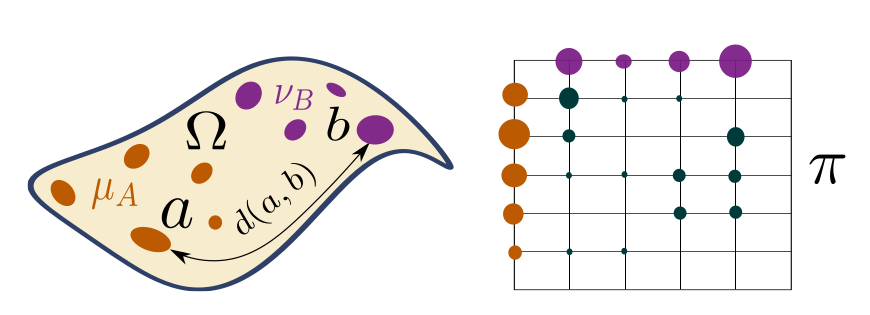
\includegraphics[width=0.3\textheight]{wd_Transportplan.png}
		\caption[Visualisierung der Wasserstein-Distanz und Transportplan]{\textbf{Links:} Visualisierung der Wasserstein-Distanz zwischen den Verteilungen $\mu_A$ und $\nu_B$ auf dem metrischen Raum $(\Omega,d)$. \textbf{Rechts:} Möglicher Transportplan $\pi$.}
		\source{\cite{vialard2019elementary}}
		\label{im:wasserstein_distance_visualization}
	\end{figure}
	
	
	
	
	\begin{remark}
		Für größere $\varepsilon$ wird mehr Entropie gefordert
	\end{remark}
	
	\begin{proposition}[Konvergenz in $\varepsilon$ \cite{COTcuturi}]
		Die eindeutige Lösung $P_\varepsilon$ von \eqref{eq:reg_problem} konvergiert gegen die optimale Lösung mit maximaler Entropie innerhalb der Menge aller optimalen Lösungen des Kan\-to\-ro\-vich-Pro\-blems, d.h.
		\begin{equation}
		\boldsymbol{P}_\varepsilon \xrightarrow{\varepsilon \to 0} \argmin_{P} \lbrace -\boldsymbol{H}(\boldsymbol{P}) : \boldsymbol{P} \in \Pi (\boldsymbol{a}, \boldsymbol{b}), \langle \boldsymbol{P}, \boldsymbol{C} \rangle = L_{\boldsymbol{C}}(\boldsymbol{a}, \boldsymbol{b}) \rbrace, \label{eq:P_eps_0} 
		\end{equation}
		
		
		\begin{equation}
		L_{\boldsymbol{C}}^\varepsilon (\boldsymbol{a}, \boldsymbol{b}) \xrightarrow{\varepsilon \to 0} L_{\boldsymbol{C}}(\boldsymbol{a}, \boldsymbol{b})
		\end{equation}
		Zudem gilt
		\begin{equation}
		\boldsymbol{P}_\varepsilon \xrightarrow{\varepsilon \to \infty} \boldsymbol{a} \otimes \boldsymbol{b} = \boldsymbol{a} \boldsymbol{b}^\top = (\boldsymbol{a}_i \boldsymbol{b}_j)_{i,j}. \label{eq:P_eps_infty}
		\end{equation}
	\end{proposition}
	
	\begin{proof}
		Sei eine Folge $(\varepsilon_l)_l$ mit $\varepsilon_l \to 0$ und $\varepsilon_l > 0$ gegeben. Sei $\boldsymbol{P}_l$ die Lösung von  \eqref{eq:reg_problem} für $\varepsilon = \varepsilon_l$. Da $\Pi(\boldsymbol{a},\boldsymbol{b})$ beschränkt ist, existiert eine Teilfolge $\varepsilon_k$ mit $\boldsymbol{P}_k \to \boldsymbol{P}^*$. Aufgrund der Abgeschlossenheit von $\Pi(\boldsymbol{a},\boldsymbol{b})$ folgt $\boldsymbol{P}^* \in \Pi(\boldsymbol{a},\boldsymbol{b})$.
		
		\noindent Sei $\boldsymbol{P} \in \Pi (\boldsymbol{a},\boldsymbol{b})$ beliebig mit $\langle \boldsymbol{C}, \boldsymbol{P} \rangle = L_C(\boldsymbol{a},\boldsymbol{b})$. Aufgrund der Optimalität von $\boldsymbol{P}$ und $\boldsymbol{P}_l$ bezüglich $L_{\boldsymbol{C}}(\boldsymbol{a},\boldsymbol{b})$ bzw. $L_{\boldsymbol{C}}^{\varepsilon_l}(\boldsymbol{a},\boldsymbol{b})$ gilt
		
		\begin{equation}
		0 \leq \langle \boldsymbol{C}, \boldsymbol{P}_l\rangle - \langle \boldsymbol{C}, \boldsymbol{P}\rangle \leq \varepsilon_l (\boldsymbol{H}(\boldsymbol{P}_l)-\boldsymbol{H}(\boldsymbol{P})). \label{eq:abschätzung1}
		\end{equation}
		Aufgrund der Stetigkeit von $\boldsymbol{H}$ folgt für $l \to +\infty$ in \eqref{eq:abschätzung1} $\langle \boldsymbol{C}, \boldsymbol{P}^* \rangle = \langle \boldsymbol{C}, \boldsymbol{P} \rangle$, womit $\boldsymbol{P}^*$ ein zulässiger Punkt ist. Division durch $\varepsilon_l$ in \eqref{eq:abschätzung1} und Übergang zum Grenzwert liefert $\boldsymbol{H}(\boldsymbol{P})\leq \boldsymbol{H}(\boldsymbol{P}^*)$. Folglich ist $\boldsymbol{P}^*$ eine Lösung von \eqref{eq:P_eps_0}.
		
		\noindent Da die Lösung $\boldsymbol{P}_0^*$ aufgrund der strikten Konvexität von $-\boldsymbol{H}$ eindeutig ist, gilt $\boldsymbol{P}^* = \boldsymbol{P}_0^*$ und die gesamte Folge konvergiert.
		
		
	\end{proof}
	
	\begin{remark}
		\eqref{eq:P_eps_0} zeigt, dass die Lösung für kleine $\varepsilon$ gegen den Transportplan mit maximaler Entropie konvergiert. Im Gegensatz dazu bedeutet \eqref{eq:P_eps_infty}, dass die Lösung für große Regularisierungsparameter gegen die Kopplung mit maximaler Entropie zwischen zwei gegebenen Randverteilungen $\boldsymbol{a}$ und $\boldsymbol{b}$ konvergiert.		
	\end{remark}
	
	\begin{remark}
		Für größere Werte von $\varepsilon$ ergibt sich eine beschleunigte Berechnung der optimalen Kopplung.
	\end{remark}
	
	\noindent \textbf{Interpretation als KL-Problem:} Das Minimierungsproblem \eqref{eq:reg_problem} kann außerdem als Spezialfall eines Kullback-Leibler-Minimierungsproblems betrachtet werden, bei dem eine Kopplungsmatrix $\boldsymbol{P}_\varepsilon$ gesucht ist, die im Sinne einer Kullback-Leibler-Divergenz möglichst nahe an einem Kernel $K$ liegt.
	Wir definieren die Kullback-Leibler-Divergenz zwischen zwei  Kopplungen \cite{COTcuturi} als
	
	\begin{equation}
	\boldsymbol{KL}(\boldsymbol{P}|\boldsymbol{K}) := \sum_{i,j} \boldsymbol{P}_{i,j} \log \left(\frac{\boldsymbol{P}_{i,j}}{\boldsymbol{K}_{i,j}} \right) - \boldsymbol{P}_{i,j} + \boldsymbol{K}_{i,j}. \label{eq:KL_div_discrete}
	\end{equation}
	Damit ist die eindeutige Lösung $\boldsymbol{P}_\varepsilon$ von \autoref{eq:reg_problem} eine Projektion des zur Kostenmatrix $\boldsymbol{C}$ gehörigen Gibbs-Kernels $\boldsymbol{K}_{i,j} := e^{-\frac{\boldsymbol{C}_{i,j}}{\varepsilon}}$ auf $\Pi (\boldsymbol{a}, \boldsymbol{b})$.
	
	\noindent Mit der obigen Definition erhalten wir
	
	\begin{equation}
	\boldsymbol{P}_\varepsilon = Proj_{\boldsymbol{\Pi} (\boldsymbol{a}, \boldsymbol{b})}^{\boldsymbol{KL}}(\boldsymbol{K}) := \argmin_{P \in \boldsymbol{\Pi} (\boldsymbol{a}, \boldsymbol{b})}{\boldsymbol{KL}(\boldsymbol{P}|\boldsymbol{K})}.
	\end{equation}
	
	\subsubsection{Algorithmus von Sinkhorn und Variationen}
	In diesem Abschnitt sehen wir, dass die Lösung des regularisierten Problems eine besondere Form besitzt, die auf den Algorithmus von Sinkhorn führt.
	
	%Matrix Scaling + einige Theoreme und Bemerkungen zu Kullback-Leibler und mehr Info \cite{vialard2019elementary}
	
	\begin{comment}
	
	\begin{remark}[Formulierung für allgemeine Maße]
	Für beliebige Maße lässt sich ebenfalls eine regularisierte Formulierung \cite{COTcuturi} angeben. 
	Dazu wird die diskrete Entropie durch die relative Entropie bezüglich des Produktmaße $d\alpha \otimes d\beta (x,y) := d\alpha (x) d\beta (y)$. Als regularisierte Version von \autoref{eq:kontorovich_allgemein} ergibt sich 
	\begin{equation}
	\min_{\pi \in \Pi (\alpha , \beta)} \int_{\mathcal{X}\times \mathcal{Y}}{c(x,y)d\pi (x,y) + \varepsilon KL(\pi |\alpha \otimes \beta)}, 
	\end{equation}\label{eq:kantorovich_reg_allgemein}
	wobei die relative Entropie eine Verallgemeinerung der diskreten Kullback-Leibler-Divergenz \autoref{eq:KL_div_discrete} ist und die folgende Form besitzt:
	\begin{align}
	KL(\pi |\xi) &:=\int_{\mathcal{X} \times \mathcal{Y}} \log \left(\frac{d\pi}{d\xi}(x,y)\right) d\pi (x,y) \\
	´			& + \int_{\mathcal{X} \times \mathcal{Y}}(d\xi (x,y) - d\pi (x,y)).			 
	\end{align}
	Hierbei wird $KL(\pi | \xi) = +\infty$ gesetzt, falls $\pi$ keine Dichte $\frac{d\pi}{d\xi}$ bezüglich $\xi$ besitzt.
	\end{remark}
	
	Die folgende Proposition zeigt, dass die Lösung von \autoref{eq:kantorovich_reg_allgemein} unabhängig von der Wahl des Referenzmaßes für die Definition von $KL(\cdot | \alpha \otimes \beta)$ ist.
	
	\begin{proposition}
	Für $\pi \in \Pi(\alpha, \beta)$ und $(\alpha ', \beta ')$, mit den selben Nullmengen wie $(\alpha , \beta )$,
	gilt
	\begin{equation}
	KL(\pi |  \alpha \otimes \beta) = KL( \pi |\alpha ' \otimes \beta ') - KL(\alpha \otimes \beta | \alpha ' \otimes \beta ')
	\end{equation}
	\end{proposition}
	
	\autoref{eq:kantorovich_reg_allgemein} kann äquivalent als Projektionsproblem
	\begin{equation}
	\min_{\pi \in \Pi (\alpha, \beta)}{KL(\pi |\mathcal{K})} \label{eq:schrödinger}
	\end{equation}
	geschrieben werden, wobei $\mathcal{K}$ die Gibbs-Verteilung $d\mathcal{K}(x,y) := e^{-\frac{c(x,y)}{\varepsilon}}d\alpha (x) d\beta (y)$ besitzt.\\
	Diese Formulierung ist auch "Statisches Schrödinger Problem" bekannt.
	Für $\varepsilon  \to 0$ konvergiert die eindeutige Lösung von \autoref{eq:schrödinger} gegen die Lösung mit maximaler Entropie von \autoref{eq:kontorovich_allgemein} \cite{carlier2017convergence}.
	\footnote{\url{https://hal.archives-ouvertes.fr/hal-00849930/document}}	
	\end{comment}
	\begin{proposition}
		Die Lösung des regularisierten Problems \eqref{eq:reg_problem} besitzt die Form
		\begin{equation}
		\forall (i,j) \in \lbrace 1,...,n \rbrace \times \lbrace 1,...,m \rbrace : \boldsymbol{P}_{i,j} = \boldsymbol{u}_i \boldsymbol{K}_{i,j} \boldsymbol{v}_j \label{eq:reg_sol_factorized}
		\end{equation}
		für die beiden (unbekannten) Variablen $(\boldsymbol{u}, \boldsymbol{v}) \in \mathbb{R}_+^n \times \mathbb{R}_+^m.$
	\end{proposition}
	
	\begin{proof}
		Wir führen für jede der beiden Nebenbedingungen die dualen Variablen $\boldsymbol{f} \in \mathbb{R}^n$ und $\boldsymbol{g} \in \mathbb{R}^m$ ein. Für die Lagrange-Funktion zu \eqref{eq:reg_problem} erhalten wir damit:
		\begin{equation}
		\mathcal{L}(\boldsymbol{P}, \boldsymbol{f}, \boldsymbol{g}) = \langle \boldsymbol{P}, \boldsymbol{C} \rangle -\varepsilon \boldsymbol{H}(\boldsymbol{P}) - 
		\langle \boldsymbol{f}, \boldsymbol{P}\boldsymbol{1}_m - \boldsymbol{a} \rangle -
		\langle \boldsymbol{g}, \boldsymbol{P}^\top \boldsymbol{1}_n - \boldsymbol{a} \rangle. 
		\end{equation}
		\noindent Mit der Optimalitätsbedingung erster Ordnung ergibt sich
		\begin{equation}
		\frac{\partial \mathcal{L} (\boldsymbol{P}, \boldsymbol{f}, \boldsymbol{g})}{\partial \boldsymbol{P}_{i,j}} = \boldsymbol{C}_{i,j} + \varepsilon \log (\boldsymbol{P}_{i,j}) -\boldsymbol{f}_i - \boldsymbol{g}_j = 0,
		\end{equation}
		
		\noindent womit wir für eine optimale Kopplung $\boldsymbol{P}$ für das regularisierte Problem den Ausdruck $\boldsymbol{P}_{i,j} = e^{\boldsymbol{f}_i/\varepsilon}e^{-\boldsymbol{C}_{i,j}/\varepsilon}e^{\boldsymbol{g}_j/\varepsilon}$ erhalten, der in die gewünschte Form umgeschrieben werden kann.
	\end{proof}
	
	
	
	\noindent Die Faktorisierung der Lösung in \eqref{eq:reg_sol_factorized} können wir in der folgenden Matrix-Form schreiben: $\boldsymbol{P} = diag(\boldsymbol{u}) \boldsymbol{K} diag(\boldsymbol{v})$. Die beiden Variablen $(\boldsymbol{u}, \boldsymbol{v})$ müssen deshalb die folgenden nichtlinearen Gleichungen erfüllen, die aufgrund der geforderten Massenerhaltungsbedingung in $\Pi (\boldsymbol{a},\boldsymbol{b})$ gelten:
		\begin{equation}
		diag(\boldsymbol{u}) \boldsymbol{K} diag(\boldsymbol{v})\boldsymbol{1}_m = \boldsymbol{a} \quad\text{ und } \quad
		diag(\boldsymbol{v}) \boldsymbol{K}^\top diag(\boldsymbol{u})\boldsymbol{1}_n = \boldsymbol{b}.
		\end{equation}
		Aufgrund der Beziehung $diag(\boldsymbol{v})\boldsymbol{1}_m =  \boldsymbol{v}$ und selbiger Beziehung für $\boldsymbol{u}$ erhalten wir die folgende Vereinfachung
		\begin{equation}
		\boldsymbol{u} \odot (\boldsymbol{K}\boldsymbol{v}) = \boldsymbol{a} \quad\text{ und }\quad
		\boldsymbol{v} \odot (\boldsymbol{K}^\top \boldsymbol{u}) = \boldsymbol{b}, \label{eq:sinkhorn_equations}
		\end{equation}  
		wobei $\odot$ für die komponentenweise Multiplikation zweier Vektoren steht. Dieses Problem ist als \textit{Matrix Scaling Problem} \cite{matrix_scaling} bekannt.\\
		
		\noindent Eine Möglichkeit zur Lösung dieses Problems ist ein iteratives Verfahren, bei dem zunächst $\boldsymbol{u}$ so modifiziert wird, dass die linke Seite in \eqref{eq:sinkhorn_equations} erfüllt ist, und anschließend die Modifikation von $\boldsymbol{v}$ vorgenommen wird, sodass die rechte Seite in \autoref{eq:sinkhorn_equations} gilt. Mit diesen beiden Modifikationen erhalten wir den Algorithmus von Sinkhorn, der aus den beiden folgenden Updates besteht:
		
		\begin{equation}
		\boldsymbol{u}^{(l+1)}:= \frac{\boldsymbol{a}}{\boldsymbol{K}\boldsymbol{v}^{(l)}} \text{ und }
		\boldsymbol{v}^{(l+1)}:= \frac{\boldsymbol{b}}{\boldsymbol{K}^\top \boldsymbol{u}^{(l+1)}}, \label{sinkhorn_iteartions}
		\end{equation} 
		wobei zu Beginn mit einem beliebigen positiven Vektor, beispielsweise ${\boldsymbol{v}^{(0)}=\boldsymbol{1}_m}$ initialisiert wird und $l$ den aktuellen Iterationsschritt bezeichnet. Die obige Division muss ebenfalls elementweise verstanden werden.
		
		\noindent Die Konvergenz dieses Verfahrens wurde zuerst von Sinkhorn \cite{sinkhorn1964relationship} gezeigt und trägt deshalb den entsprechenden Namen.
	
	
	
	\begin{comment}
	The iterations (4.15) first appeared in [Yule, 1912,
	Kruithof, 1937]. They were later known as the iterative proportional fitting procedure
	(IPFP) Deming and Stephan [1940] and RAS [Bacharach, 1965] methods [Idel, 2016].
	The proof of their convergence is attributed to Sinkhorn \cite{sinkhorn1964relationship}, hence the name of the
	algorithm.
	\end{comment}
	
	
	
	
	\begin{remark}
		Die Lösung des regularisierten Problems lässt sich nach der L-ten Sinkhorn-Iteration mit dem Transportplan wie folgt angeben: $P_L = diag(u_L)K diag(v_L)$. Die Gesamtkosten sind gegeben durch\\
		\noindent $\langle P_L, C_{XY}\rangle~=~u_L ^\top ( K \odot~ C_{XY})v_L$.	\end{remark}	
	
	
	\noindent Für die globale Konvergenzanalayse der Sinkhorn-Algorithmus lässt sich alternativ zum Beweis in \cite{sinkhorn1964relationship} ein Zusammenhang mit der Hilbertschen Projektionsmetrik benutzen, der erstmals in \cite{franklin_sinkhorn_convergence} vorgestellt wurde. Diese ist wie folgt definiert.
	
	\begin{definition}[Projektive Hilbert-Metrik]
		Seien $u,u' \in \mathbb{R}_{+,\star}^n$.
		Dann ist die projektive Hilbert-Metrik $d_\mathcal{H}$ definiert durch
		\begin{equation}
		d_\mathcal{H}(u,u') := \log \max_{i,j}{\frac{u_iu_j'}{u_ju_i'}}.
		\end{equation}
	\end{definition}
	
	\begin{remark}
		Die Hilbert-Metrik $ d_\mathcal{H}$ definiert eine Metrik auf dem projektiven Kegel $\mathbb{R}_{+, \star}^n/\sim$, wobei $u \sim u'$ bedeutet, dass gilt: $\exists r >0:u=ru'$, d.h. die Vektoren $u$ und $u'$ sind bis auf Skalierung identisch.
		
	\end{remark}
	
	\begin{comment}
	The Hilbert metric was introduced independently by [Birkhoff,
	1957] and [Samelson et al., 1957]. They proved the following fundamental theorem,
	which shows that a positive matrix is a strict contraction on the cone of positive
	vectors.
	\end{comment}
	
	
	\noindent Das folgende Theorem zeigt, dass eine positive Matrix eine Kontraktion auf dem Kegel positiver Vektoren bezüglich der Hilbert-Metrik ist.
	
	\begin{theorem}\label{theorem41}
		Sei $K \in \mathbb{R}_{+,\star}^{n \times m}$. Dann gilt für $(v,v') \in (\mathbb{R}_{+, \star}^m)^2$
		
		\begin{equation}
		d_\mathcal{H}(Kv,Kv') \leq \lambda (K) d_\mathcal{H}(v,v'), \text{ mit } \begin{cases}
		\lambda (K) := \frac{\sqrt{\nu (K)} -1}{\sqrt{\nu (K)}+1}\\
		\nu (K) := \max_{i,j,k,l} \frac{K_{i,k}K_{j,l}}{K_{j,k}K_{i,l}}.
		
		\end{cases}
		\end{equation}
	\end{theorem}
	
	%Visualisierung des Theorems vgl \cite{COTcuturi},Seite 70.
	
	\noindent Mit dem folgenden Resultat erhalten wir die Konvergenz des Sinkhorn-Verfahrens:
	
	\begin{theorem}\cite{COTcuturi}
		Es gilt $(u^{(l)}, v^{(l)})\to (u^\star, v^\star)$  für $(u^{(l)}, v^{(l)})$ in \eqref{sinkhorn_iteartions} und
		\begin{equation}
		d_{\mathcal{H}}(u^{(l)}, u^\star) = \mathcal{O}(\lambda(K)^{2l}), \qquad d_\mathcal{H}(v^{(l)},v^\star) = \mathcal{O}(\lambda (K)^{2l}) \label{eq:erstesResThm42}
		\end{equation}
		Es gelten außerdem die beiden folgenden Abschätzungen
		\begin{align}
		d_\mathcal{H} (u^{(l)}, u^\star) &\leq \frac{d_\mathcal{H}(P^{(l)}\boldsymbol{1}_m, a)}{1-\lambda(K)^2}, \label{eq:thm42zweiAbschätzungen1}\\
		d_\mathcal{H} (v^{(l)}, v^\star) &\leq \frac{d_\mathcal{H}(P^{(l)\top}\boldsymbol{1}_n, b)}{1-\lambda(K)^2}, \label{eq:thm42zweiAbschätzungen}		
		\end{align}
		wobei \begin{equation}
		P^{(l)} := diag(u^{(l)})K diag(v^{(l)}) \label{eq:reconstruction_TransportPlan}
		\end{equation}
		gilt. Desweiteren gilt die Abschätzung
		\begin{equation}
		|| \log(P^{(l)}) - \log (P^\star)||_\infty \leq d_\mathcal{H} (u^{(l)}, u^\star) + d_\mathcal{H} (v^{(l)}, v^\star), \label{eq:thm42letzteAbschätzung}
		\end{equation}
		wobei $P^\star$ die eindeutige Lösung von \autoref{eq:reg_problem} ist.
	\end{theorem}
	\begin{proof}
		Für ein beliebiges Paar $(v,v') \in (\mathbb{R}_{+,\star}^m)^2$ gilt
		\begin{equation*}
		d_\mathcal{H} (v,v') = d_\mathcal{H}(v/v',\boldsymbol{1}_m) = d_\mathcal{H}(\boldsymbol{1}_m/v,\boldsymbol{1}_m/v').
		\end{equation*}
		Mit dieser Beziehung und \autoref{theorem41} erhalten wir
		\begin{align*}
		d_\mathcal{H}(u^{(l+1)}, u^\star) &= d_\mathcal{H}\left(\frac{a}{Kv^{(l)}},\frac{a}{Kv^\star}\right)\\
		&=d_\mathcal{H}(Kv^{(l)}, Kv^\star) \\
		&\leq \lambda (K)d_\mathcal{H}(v^{(l)},v^\star).
		\end{align*}
		Dies zeigt \eqref{eq:erstesResThm42}. Mit Hilfe der Dreiecksungleichung erhalten wir
		\begin{align*}
		d_\mathcal{H}(u^{(l)}, u^\star) &\leq d_\mathcal{H}(u^{(l+1)},u^{(l)}) + d_\mathcal{H}(u^{(l+1)},u^\star)\\
		& \leq d_\mathcal{H}\left(\frac{a}{Kv^{(l)}}, u^{(l)}\right) + \lambda (K)^2 d_\mathcal{H}(u^{(l)},u^\star)\\
		&= d_\mathcal{H}\left(a, u^{(l)} \odot (Kv^{(l)})\right) + \lambda (K)^2 d_\mathcal{H}(u^{(l)},u^\star)\\
		&= d_\mathcal{H}\left(a, P^{(l)}\boldsymbol{1}_m \right) + \lambda (K)^2 d_\mathcal{H}(u^{(l)},u^\star)
		\end{align*}
		Nach Division durch $1-\lambda(K)^2$ erhalten wir  \autoref{eq:thm42zweiAbschätzungen1}. Die zweite Abschätzung
		\eqref{eq:thm42zweiAbschätzungen} folgt analog. 
		Die \autoref{eq:thm42letzteAbschätzung} gilt nach Lemma 3 in \cite{franklin_sinkhorn_convergence}.
	\end{proof}
	
	\begin{comment}
	
	\begin{remark}
	\leavevmode 
	\begin{itemize}
	\item Konvergenzrate?
	\item Berechnung der optimalen Transportpläne mit \autoref{eq:reconstruction_TransportPlan} im Zeitschritt $l$ und Berechnung der Transportkosten ...
	\item Abbruchkriterien (vgl. mit der POT Implementierung)
	\end{itemize}
	\end{remark}
	content...
	\end{comment}
	\subsubsection{Komplexitätsanalyse}
	Altschuler \cite{altschuler2017near} liefert eine Komplexitätsanalyse für die Sinkhorn-Iterationen. Im Fall $n=m$ sind für die Wahl $\varepsilon = \frac{4 \log (n)}{\tau}$ $\mathcal{O}(||C||_\infty^3 \log (n)\tau ^{-3})$ Sinkhorn-Iterationen (inklusive eines Rundungsschrittes) notwendig, um eine zulässige Kopplung $\hat{\boldsymbol{P}} \in \Pi(\boldsymbol{a}, \boldsymbol{b})$ zu berechnen, die die Abschätzung \\ $\langle \hat{\boldsymbol{P}}, \boldsymbol{C} \rangle \leq L_{\boldsymbol{C}}(\boldsymbol{a}, \boldsymbol{b}) +  \tau$ erfüllt. Somit liefert das Sinkhorn-Verfahren eine $\tau$-Approximation des nicht regularisierten Problems in $\mathcal{O}(n^2 \log (n)\tau ^{-3})$ Operationen.
	Gleichzeitig wird dort eine Greedy-Variante der Sinkhorn-Iterationen namens Greenkhorn präsentiert, die eine $\tau$-Ap\-pro\-xi\-ma\-tion in $\mathcal{O}(n^2\tau^{-3})$ Operationen liefert.
	\cite{dvurechensky2018computational} verbessert diese auf $\mathcal{O}(n^2\tau^{-2})$ Operationen.
	\subsection{Gromov-Wasserstein-Distanz}\label{gwd}
	In den vorherigen Abschnitten hatten wir jeweils Wahrscheinlichkeitsmaße auf demselben metrischen Raum verglichen. In diesem Abschnitt wollen wir diesen Abstandsbegriff auf die Distanz zweier verschiedener metrischer Maßräume verallgemeinern. Dazu definieren wir die \acf{gwd}, die der Wasserstein-Distanz sehr ähnlich und eine Relaxierung der Hausdorff-Distanz ist. Dabei folgen wir \cite{COTcuturi}, \cite{vayer2020contribution}, \cite{vayer2020fused}, \cite{gwd_averaging_kernels}.
	
	\subsubsection{Gromov-Wasserstein-Distanz}
	In diesem Abschnitt wollen wir nun den Begriff der Wasserstein-Distanz auf einen Distanzbegriff für zwei verschiedene Grundräume metrischer Maßräume verallgemeinern.
	
	\begin{definition}[Tensor-Matrix-Multiplikation]
		Für einen Tensor $\mathcal{L} = (\mathcal{L}_{i,j,k,l})_{i,j,k,l}$ und eine Matrix $(T_{i,j})_{i,j}$ definieren wir die Tensor-Matrix-Mul\-ti\-pli\-ka\-tion als
		\begin{equation}
		\mathcal{L} \otimes T := \left(\sum_{k,l}{\mathcal{L}_{i,j,k,l}T_{k,l}}\right)_{i,j}. \label{eq:tensor_matrix_mul}
		\end{equation}
	\end{definition}
	%\cite{vialard2019elementary}
	\noindent Wir definieren zunächst die beiden folgenden Distanzen:
	
	\begin{definition}[Hausdorff-Metrik]
		Sei $\mathscr{X}$ ein metrischer Raum.
		Für  $X,Y \subset \mathscr{X}$ kompakt und nichtleer definieren wir die \emph{Hausdorff-Metrik} $d_H(X,Y)$ als
		\begin{equation}
		d_H(X,Y) = \max \lbrace \sup_{x \in X} \inf_{y \in Y} d(x,y), \sup_{y \in Y} \inf_{x \in X} d(x,y) \rbrace .
		\end{equation} 
		
	\end{definition}
	\noindent Anschaulich haben zwei kompakte Teilmengen einen geringen Hausdorff-Abstand, wenn es zu jedem Element der einen Menge ein Element der anderen Menge gibt, zu dem dieses einen geringen Abstand hat. In \autoref{im:hausdorff_example} ist die Hausdorff-Distanz zweier Mengen $X$ und $Y$ dargestellt.
	
	\begin{figure}[!ht]
		\centering
		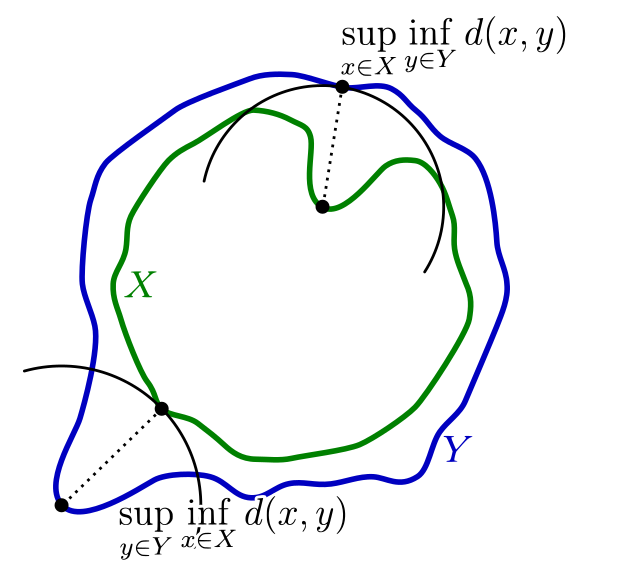
\includegraphics[width=0.3\textheight]{Hausdorff_distance.png}
		\caption{Visualisierung der Hausdorff-Distanz zwischen den Mengen $X$ und $Y$ in $\mathbb{R}^2$.}
	
		\label{im:hausdorff_example}	
		\source{\cite{hausdorffpict}}
	\end{figure}
	
	
	\noindent Eine Teilmenge $R \subset X \times Y$ ist eine Korrespondenz zwischen den Mengen $X$ und $Y$, falls $\pi_1(R) = X$ und $\pi_2(R) = Y$, wobei $\pi_1: X \times Y \to X$ und $\pi_2: X \times Y \to Y$ die kanonischen Projektionen sind. Sei $\mathcal{R}(X,Y)$ die Menge aller Korrespondenzen zwischen $X$ und $Y$.
	
	\begin{definition}[Gromov-Hausdorff-Metrik]
		Für die kompakten, metrischen Räume $(X,d_X)$ und $(Y,d_Y)$ ist die \emph{Gromov-Hausdorff-Metrik} definiert als
		\begin{equation}
		d_{\mathcal{G}\mathcal{H}}(X,Y) = \frac{1}{2}\inf_{R} \sup_{(x,y),(x',y') \in R}{|d_X(x,x')- d_Y(y,y')|}, \label{eq:gh}
		\end{equation}
		wobei $R$ über ganz $\mathcal{R}(X,Y)$ reicht.
	\end{definition}
	
	\noindent Sei nun $p\geq 1$. Für zwei metrische Maßräume $(X,d_X,\mu_X)$ und $(Y,d_Y,\mu_Y)$ betrachten wir die Funktion 
	\begin{equation}
	L(x,y,x',y') = |d_X(x,x') - d_Y(y,y')|
	\end{equation}
	und definieren die \ac{gwd} der Ordnung $p$ \cite{memoli2011gromov}:
	\begin{equation}
	d_{\mathcal{GW},p}(\mu_X,\mu_Y):=\left(\inf_{\pi \in \Pi(\mu_X, \mu_Y)} {J_p(\pi)}\right)^{1/p},
	\end{equation}
	wobei
	\begin{equation}
	J_p(\pi) := \int\limits_{X\times Y \times  X\times Y}{L(x,y,x',y')^pd\pi(x,y)d\pi(x',y')}
	\end{equation}
	gilt und $\Pi(\mu_X,\mu_Y) = \lbrace \pi \in P(X\times Y) | \forall (X_0,Y_0) \in X \times Y, \pi (X_0 \times Y) = \mu_X (X_0), \pi(X \times Y_0) = \mu_Y(Y_0) \rbrace$
	die Menge der Kopplungen der beiden Maßräume $(X,\mu_X)$ und $(Y,\mu_Y)$ ist \cite{villani2003topics,vayer2020fused}.
	\begin{remark}
		Mit dieser Definition erhalten wir nun eine relaxierte $L^p$-Version der Gromov-Hausdorff-Metrik \eqref{eq:gh}.
	\end{remark}
	\noindent Die \ac{gwd} definiert eine Metrik auf dem Raum aller metrischen Räume $\mathcal{M}^{iso}$. 
	Mit dieser Definition wir der Vergleich von Maßen über unterschiedlichen Grundräumen möglich und damit auch ein Vergleich von Objekten jeglicher Art.
	
	\begin{figure}[h!]
		\begin{center}
			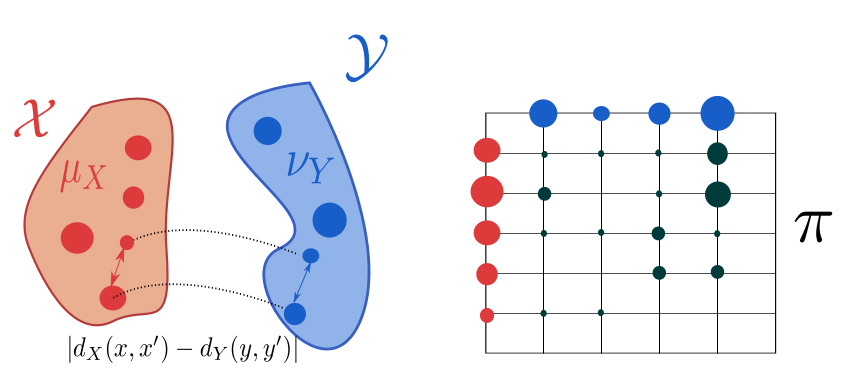
\includegraphics[width=0.3\textheight]{gwd_Transportplan.png}
			\caption[Beispiel der \acl{gwd}]{\textbf{Links:} Die beiden metrischen Maßräume $\mathcal{X}$ und $\mathcal{Y}$. \textbf{Rechts:} Zugehöriger Transportplan}
			\source{\cite{vayer2020fused}}
		\end{center}
	\end{figure}
	\newpage
	\noindent Wir zitieren einige Eigenschaften der \ac{gwd}:
	
	\begin{theorem}\cite[Thm. 5.1]{memoli2011gromov} Sei $p \in [1, \infty].$ Dann gilt:
		\begin{itemize}
			\item[(a)] $d_{\mathcal{GW},p}$ definiert eine Metrik auf der Menge aller Isomorphieklassen von metrischen Maßräumen. 
			\item[(b)] (Zwei Wahrscheinlichkeitsmaße auf demselben Raum) Sei $(Z,d)$ ein kompakter metrischer Raum und $\alpha$ und $\beta$ zwei verschiedene Borel-Maße auf $Z$. Sei $X=(Z,d,\alpha)$ und $Y=(Z,d,\beta)$. Dann gilt
			\begin{equation}
			d_{\mathcal{GW},p}(X,Y) \leq d_{\mathcal{W},p}^Z(\alpha,\beta).
			\end{equation}
		\end{itemize}
		
	\end{theorem}
	
	\noindent Dieses Theorem zeigt nun, dass wir mit der \ac{gwd} einen Distanzbegriff erhalten, der invariant gegenüber Rotationen, Translationen und Permutationen ist\cite{vayer2020contribution}. \\
	
	\noindent Aufgrund genau dieser Invarianz vermuten wir, dass dieser Distanzbegriff deutlich besser als eine pixelweise $L_2$-Distanz für ein Clustering auf der Grundlage von Heatmaps ist, wie wir es in \autoref{chapter:algorithm} benutzen werden. Diese Invarianz resultiert daraus, dass wir eine Metrik auf den Isomorphie-Klassen metrischer Maßräume betrachten.\\
	
	\noindent Im Folgenden werden wir die numerischen Verfahren zur Bestimmung der \ac{gwd} behandeln. Auch hier ermöglicht eine Entropie-regularisierte Version die einfache Berechnung einer Approximation wie im Fall der Wasserstein-Distanz.\\
	
	\noindent Wir betrachten dazu wieder die diskreten Wahrscheinlichkeitsmaße \\$\mu = \sum_{i=1}^n{a_i\delta_{x_i}},$ $\nu = \sum_{j=1}^m{b_j\delta_{y_j}}$ auf den Räumen $(X,d_X)$ bzw. $(Y,d_Y)$. Mit $\boldsymbol{C}_1$ und $\boldsymbol{C}_2$ bezeichnen wir die Distanzmatrizen der paarweisen Distanzen aller Punkte innerhalb des entsprechenden Raumes, d.h. es gilt \begin{equation}
		\forall (i,k) \in \lbrace 1,...,n \rbrace^2 : C_1(i,k) = d_X(x_i,x_k)
	\end{equation} und	
	
	\begin{equation}
		\forall (j,l) \in \lbrace 1,...,m \rbrace^2 : C_1(j,l) = d_Y(x_j,x_l).
	\end{equation} Damit lautet das Gromov-Wasserstein-Problem im diskreten Fall:
	
	\begin{align}
	GW_p^p(\boldsymbol{C}_1, \boldsymbol{C}_2,\boldsymbol{a},\boldsymbol{b}) &= \min_{P \in \Pi(\boldsymbol{a}, \boldsymbol{b})}\sum_{i,j,k,l}{|C_1(i,k)- C_2(j,l)|^pP_{i,j}P_{k,l}}\\
	&=\min_{P \in \Pi(\boldsymbol{a}, \boldsymbol{b})} \langle \boldsymbol{L}(\boldsymbol{C}_1, \boldsymbol{C}_2)^p \otimes P, P\rangle_\mathcal{F},\label{eq:GW-Problem}
	\end{align}
	
	\noindent wobei $\langle .,.\rangle_\mathcal{F}$ das Matrix-Produkt $\langle \boldsymbol{P}, \boldsymbol{Q} \rangle_\mathcal{F}  = tr(\boldsymbol{Q}^\top\boldsymbol{P})$ bezeichnet und \\ $\boldsymbol{L}(\boldsymbol{C}_1, \boldsymbol{C}_2) = (|C_1(i,k)-C_2(j,l)|)_{i,j,k,l}$ gilt. $\boldsymbol{L} \otimes P$ ist die Tensor-Matrix-Multiplikation nach \eqref{eq:tensor_matrix_mul}.
	
	\noindent Das Problem \eqref{eq:GW-Problem} ist ein nicht-konvexes quadratisches Optimierungsproblem, das im Allgemeinen NP-schwierig zu lösen und ebenfalls schwer zu approximieren ist.\\
	
	\noindent Sei $\mathcal{L}(C_1,C_2) := (L(C_{1_{i,k}}, C_{2_{j,l}}))_{i,j,k,l}$. Dann erhalten wir mit der folgenden Propsition eine vereinfachte Darstellung für eine bestimmte Klasse von Verlustfunktionen.
	
	
	\begin{proposition}\cite{gwd_averaging_kernels}
		Für die Verlustfunktion $L$ gelte die Darstellung
		\begin{equation}
			L(a,b) = f_1(a) + f_2(b) - h_1(a)h_2(b) \label{eq:losscondition}
		\end{equation}
		\noindent für die Funktionen $f_1,f_2,h_1,h_2$, dann gilt für $P \in \Pi(\boldsymbol{a}, \boldsymbol{b})$
		\begin{equation}
			\mathcal{L}(C_1,C_2) \otimes P = \boldsymbol{c}_{\boldsymbol{C}_1,\boldsymbol{C}_2}-h_1(C_1)Ph_2(C_2)^\top, \label{prop:loss_reformulated}
		\end{equation}
		wobei $\boldsymbol{c}_{\boldsymbol{C}_1,  \boldsymbol{C}_2}:= f_1(\boldsymbol{C}_1)\boldsymbol{a} \boldsymbol{1}_{N_2}^T + \boldsymbol{1}_{N_1}\boldsymbol{b}^Tf_2(\boldsymbol{C}_2)^T$ unabhängig von $P$ ist.	
	\end{proposition}
	
\noindent Für $p=2$ und damit $\boldsymbol{L}=|\cdot|^2$ können wir \eqref{eq:GW-Problem} schreiben als:
	
	\begin{equation}
	\min_{P \in \Pi(\boldsymbol{a}, \boldsymbol{b})}{tr(\boldsymbol{c}_{\boldsymbol{C}_1,  \boldsymbol{C}_2}P^\top) - 2 tr(\boldsymbol{C}_1P\boldsymbol{C}_2P^\top)}.
	\end{equation}
	
	\noindent In Standardform erhalten wir
	
	\begin{equation}
	\min_{\pi \in \Pi(\boldsymbol{a}, \boldsymbol{b})}{\boldsymbol{c}^\top \boldsymbol{x}(\boldsymbol{\pi}) + \frac{1}{2}\boldsymbol{x}(\boldsymbol{\pi})^\top \boldsymbol{Q}\boldsymbol{x}(\boldsymbol{\pi})},	 \label{eq:GW_p2}		
	\end{equation}
	wobei $\boldsymbol{x}(P) = vec(P), \boldsymbol{c}= vec(\boldsymbol{c}_{\boldsymbol{C}_1, \boldsymbol{C}_2})$ und $\boldsymbol{Q} = -4 \boldsymbol{C}_1 \otimes_K \boldsymbol{C}_2$ gilt. $\otimes_K$ ist das Kronecker-Matrix-Produkt für $\boldsymbol{A} \in \mathbb{R}^{n\times m}, \boldsymbol{B} \in \mathbb{R}^{p\times q}, \boldsymbol{A}\otimes_K \boldsymbol{B} \in \mathbb{R}^{np \times mq}$ mit $\boldsymbol{A} \otimes_K \boldsymbol{B} = (A_{i,j}\boldsymbol{B})_{i,j}$. \\
	
	\noindent \eqref{eq:GW_p2} ist ein nicht konvexes quadratisches Optimierungsproblem, da die Hesse-Matrix $\boldsymbol{Q}$ im Allgemeinen nicht positiv semi-definit ist (die Eigenwerte sind die Produkte der Eigenwerte der Matrizen $\boldsymbol{C}_1$ und $\boldsymbol{C}_2)$.\\
	
	%TODO: Erklärung der KL-Divergenz:
	%\url{http://people.csail.mit.edu/jsolomon/assets/gw.pdf}
	
	\subsubsection{Entropisch regularisierte Gromov-Wasserstein-Distanz} \label{chapter:GW_regularized}
	
	\noindent Verwenden wir nun auch hier einen Regularisierungs-Term basierend auf der Entropie erhalten wir als regularisierte Version von \eqref{eq:GW-Problem} das folgende Optimierungsproblem:
	
	\begin{align}
	GW_{\varepsilon}(\boldsymbol{C}_1,\boldsymbol{C}_2,\boldsymbol{a},\boldsymbol{b}) &= \min_{P \in \Pi (\boldsymbol{a} , \boldsymbol{b})}{\langle \boldsymbol{L}(\boldsymbol{C}_1, \boldsymbol{C}_2)^p \otimes P, P \rangle_\mathcal{F} - \varepsilon H(P)}\\ \label{eq:GWprob_regularised2}
	&= \min_{P \in \Pi (\boldsymbol{a} , \boldsymbol{b})} \boldsymbol{\mathcal{E}}_{\boldsymbol{C}_1, \boldsymbol{C}_2}(P) -\varepsilon H(P)
	\end{align}
	
	\noindent für 
	\begin{equation}
		\mathcal{E}_{\boldsymbol{C}_1,\boldsymbol{C}_2}(P) = \langle \boldsymbol{L}(\boldsymbol{C}_1,\boldsymbol{C}_2)^p \otimes P, P \rangle
	\end{equation}
	
	\noindent Dieses nicht-konvexe Optimierungsproblem können wir mithilfe eines projektiven Gradienten-Verfahrens lösen, bei dem sowohl für den Gradienten-Schritt als auch die Projektion die KL-Divergenz verwendet wird \cite{gwd_averaging_kernels}.\\
	
	\noindent Die Iterationen sind gegeben durch
	\begin{equation}
	P \leftarrow Proj_{\Pi(\boldsymbol{a},\boldsymbol{b})}^{KL} \left(P \odot e^{-\tau( \nabla \boldsymbol{\mathcal{E}}_{\boldsymbol{C}_1, \boldsymbol{C}_2}(P) -\varepsilon \nabla H(P))} \right), \label{iteration_projection1}
	\end{equation}
	wobei die Schrittweite $\tau > 0$ und die KL-Projektion einer beliebigen Matrix $K$ gegeben ist durch:
	\begin{equation}
	Proj_{\Pi(\boldsymbol{a},\boldsymbol{b})}^{KL}(K) := \argmin_{P \in \Pi (\boldsymbol{a},\boldsymbol{b})} KL(P|K).
	\end{equation}
	
	\noindent Es gilt außerdem
	\begin{equation}
	\nabla \boldsymbol{\mathcal{E}}_{C_1, C_2}(P) -\varepsilon \nabla H(P) = 2\boldsymbol{L}(\boldsymbol{C}_1,\boldsymbol{C}_2) \otimes P + \varepsilon\log (P).
	\end{equation}
	
	\noindent Für den Fall $\tau= 1/\varepsilon$ wird aus der Iterationsvorschrift \eqref{iteration_projection1} die Lösung des entropisch regularisierten Transportproblems nach \eqref{eq:reg_problem} mit den Grundkosten $2\boldsymbol{L}(\boldsymbol{C}_1, \boldsymbol{C}_2)^p \otimes P$ \cite{gwd_averaging_kernels}.
		
		
	
	
	\begin{comment}
	
	
	\begin{definition}[Divergenz]
	Sei $S$ der Raum aller Wahrscheinlichkeitsverteilungen mit gemeinsamem Support. Dann bezeichnet die Divergenz auf $S$ eine Funktion $D(\cdot || \cdot):S \times S \to \mathbb{R}$, für die gilt:
	\begin{enumerate}
	\item $D(p || q) \geq 0$ f.a. $p,q \in S$\\
	\item $D(p || q) = 0$ gdw. $p = q$.
	\end{enumerate}
	\end{definition}
	\end{comment}
	
	
	%egin{definition}[Entropie]
	%	Für $T \in \mathbb{R}_{+}^{N \times N}$ definieren wir die Entropie als
	%		\begin{equation}
	%		H(T) := - \sum_{i,j=1}^N{T_{i,j}(log(T_{i,j})-1)}.
	%		\end{equation}
	%	\end{definition}
	
	%Warum wir GW-Distanz brauchen
	%\url{https://arxiv.org/pdf/1811.02834.pdf}
	
	\begin{comment}
	
	Der Vergleich zwischen Ähnlichkeits- bzw. Distanzmatrizen ist schwierig, da diese die innere Struktur eines Datensatzes beschreiben, die unabhängig von Rotationen und Translationen ist. Es existiert keine kanonische Ordnung der Reihen und Spalten.
	Verallgemeinerung auf beliebige  Matrizen C, d.h. diese Distanzmatrizen müssen nicht notwendigerweise positiv sein und die Dreiecksungleichung erfüllen.
	content...
	\end{comment}
	
	
	\begin{comment}
	\noindent Häufig verwendete Fehlerfunktionen sind die quadratische Fehlerfunktion $L(a,b) = L_2(a,b) := \frac{1}{2}|a-b|^2$ und die Kullback-Leibler-Divergenz $L(a,b)  = KL(a|b) := a\log(a/b) -a+b$.\\
	
	\noindent Diese Definition der Gromov-Wasserstein-Distanz verallgemeinert die Version in \cite{gwd_averaging_kernels}, da nun beliebige Fehlerfunktionen betrachtet werden.\\
	
	
	
	\noindent Mit der folgenden Proposition ergibt sich eine effizientere Berechnung von $\boldsymbol{L}(\boldsymbol{C}_1, \boldsymbol{C}_2)^p \otimes P$ in \autoref{eq:GWprob_regularised2} für eine bestimmte Klasse von Fehlerfunktionen $L$:
	
	\begin{proposition}
		Die Fehlerfunktion $L$ lasse sich schreiben als 
		\begin{equation}
		L(a,b) = f_1(a) + f_2(b) - h_1(a)h_2(b) \label{eq:L_darstellung}
		\end{equation}
		für $f_1, f_2,h_1, h_2:\mathbb{R} \to \mathbb{R}$. Dann gilt für $T \in \Pi (p,q)$:
		\begin{equation}
		L (C_1, C_2) \otimes P = c_{C_1, C_2} - h_1(C)Ph_2(\bar{C})^T. \label{eq:berechnung_tensorprodukt}
		\end{equation}
	\end{proposition} 
		
	\end{comment}
	
	
	\begin{comment}
	\begin{proof}
	Aufgrund von \autoref{eq:L_darstellung} gilt nach der Tensor-Matrix-Multiplikation \autoref{eq:tensor_matrix_mul}
	die Zerlegung $\mathcal{L} (C, \bar{C}) \otimes T = A + B + C$ mit
	
	\begin{align*}
	A_{i,j} &= \sum_k{f_1(C_{i,k})} \sum_l{T_{k,l}} = (f_1(C)(T\boldsymbol{1}))_i, \\
	B_{i,j} &= \sum_l{f_2(\bar{C}_{j,l})} \sum_k{T_{k,l}} = (f_2(\bar{C})(T^\top\boldsymbol{1}))_j,\\
	C_{i,j} &= \sum_k{h_1(C_{i,k})} \sum_l{h_2(\bar{C}_{j,l})T_{k,l}}.
	\end{align*}
	Dies ist äquivalent zu $(h_1(C))(h_1(\bar{C}T^\top)^\top)_{i,j}.$\\
	(? Wie folgt daraus die Behauptung)
	\end{proof}
	\end{comment}
	
	
	
	\begin{remark}[Verbesserte Komplexität]
		Mit dem Resultat in \autoref{prop:loss_reformulated} können wir $\boldsymbol{L} (\boldsymbol{C}_1, \boldsymbol{C}_2) \otimes P$ effizient in der Größenordnung $\mathcal{O}(N_1^2N_2 + N_2^2N_1)$ mit ausschließlich Matrix/Matrix-Multiplikationen berechnen im Unterschied zur Komplexität von $\mathcal{O}(N_1^2N_2^2)$ für die Implementierung von \eqref{eq:tensor_matrix_mul}.
	\end{remark}
	\begin{comment}
	\begin{remark}[Spezialfälle]
		Im Fall $L=L_2$ ist die Bedingung \autoref{eq:L_darstellung} für die Funktionen $f_1(a) = a^2, f_2(b) = b^2, h_1(a) = a$ und $h_2(b) = 2b$ erfüllt.
		Für $L=KL$ sind die Funktionen $f_1(a) = a \log (a) -a, f_2(b) = b, h_1(a) =a $ und $h_2(b) = \log (b)$ notwendig.
	\end{remark}
	
	
	%Wir betrachten nun die regularisierte Version der Gromow-Wasserstein-Diskrepanz \ref{GWD_definition} und definieren:
	
	
	
	\noindent Wir erhalten damit ein nicht-konvexes Optimierungsproblem. Für dessen Lösung benutzen wir ein projektives Gradienten-Verfahren, bei dem sowohl die Schrittweite als auch die Projektion bezüglich der KL-Metrik berechnet werden.\\
	
	\noindent Die Iterationen sind gegeben durch
	\begin{equation}
	P \leftarrow Proj_{\Pi(p,q)}^{KL} \left(P \odot e^{-\tau( \nabla \boldsymbol{\mathcal{E}}_{C, \bar{C}}(P) -\varepsilon H(P))} \right), \label{iteration_projection}
	\end{equation}
	wobei die Schrittweite $\tau > 0$ und die KL-Projektion einer beliebigen Matrix $K$ gegeben ist durch:
	\begin{equation}
	Proj_{\Pi(p,q)}^{KL}(K) := \argmin_{P \in \Pi (p,q)} KL(P|K).
	\end{equation}
	
	\begin{proposition} \label{prop:iteration_GW_eps}
		Für den Fall $\tau= 1/\varepsilon$ erhalten wir die Iterationsvorschrift
		\begin{equation}
		P \leftarrow L_{L (C_1,C_2) \otimes P}(p,q). \label{simple_iteration}
		\end{equation}
		
		
	\end{proposition}
	% TODO: Hier in Prop 2kommt wohl noch der Faktor 2 rein: vgl. POT Implementerung
	\begin{proof}
		
		
		\noindent Es gilt außerdem
		\begin{equation}
		\nabla \boldsymbol{\mathcal{E}}_{C_1, C_2}(P) -\varepsilon H(P) = L(C_1,C_2) \otimes P + \varepsilon\log (P ).
		\end{equation}
		Durch Umordnen der Terme in \autoref{iteration_projection} erhalten wir für $\tau \varepsilon = 1$ die angegebene Vorschrift.
	\end{proof}
	\end{comment}
	\begin{remark}
		Die Iterationsvorschrift \ref{iteration_projection1} definiert damit einen einfachen Algorithmus, der in jedem Update von $P$ eine Sinkhorn-Projektion benötigt.
	\end{remark}
	\begin{comment}
	
	\begin{remark}[Konvergenz]
	Die Iterationen \autoref{iteration_projection} konvergieren nach \cite{boct2016inertial} für $\tau < \tau_{max}$. Im Allgemeinen gilt $1/\varepsilon < \tau_{max}$ jedoch nicht, womit die Wahl der Schrittweite $\tau = 1 $ in \autoref{prop:iteration_GW_eps} nicht durch die Theorie abgedeckt ist. Laut \cite{gwd_averaging_kernels} konvergiert die Iteration mit $\tau = 1/\varepsilon$ jedoch in der Praxis.\\
	Für den Fall $L=L_2$ ergibt sich der \textit{Softassign quadratic assignment algorithm} \cite{rangarajan1999convergence}, für welchen ein Konvergenzresultat im Fall eines konvexen Problems existiert. Da wir in unserem Fall nur positive symmetrische Matrizen $C,C_s$ betrachten ist hier die Konvergenz gesichert.
	\end{remark}
	content...
	\end{comment}
	
	
	\begin{remark}
		Für gewöhnlich wählt man die Schrittweite $ \tau$ im Gradientenverfahren nicht zu groß, um die Konvergenz des Verfahrens zu erhalten. Da die Schrittweite $\tau$ hier jedoch antiproportional zum Regularisierungs-Parameter $\varepsilon$ ist, gibt es einen Trade-off zwischen der Konvergenz des Verfahrens und einer Unschärfe in der optimalen Lösung. 
	\end{remark}

	%TODO: Definition von entropisch regularisierte GWD
	
	
	\subsubsection{Gromov-Wasserstein Baryzentren}
	In diesem Kapitel wollen wir uns mit dem \glqq Mittelwert\grqq{} befassen, der elementar für das $k$Means-Clustering (\autoref{chapter:kMeans}) ist.
	Auch hier soll der Mittelwert auf die abstrakte Ebene von gewichteten Distanzmatrizen angehoben werden.
	Dazu definieren wir im Folgenden sogenannte Wasserstein-Baryzentren und folgen \cite{gwd_averaging_kernels} für die Lösung des entstehenden Optimierungsproblems.
	%Gute Einführung\footnote{\url{https://hal.archives-ouvertes.fr/hal-00637399/document}}
	\begin{definition}[Gromov-Wasserstein Baryzentrum]
		Seien die mit $(\lambda_s)_s$ gewichteten Distanzmatrizen $(C_s)_{s=1}^S$, mit $C_s \in \mathbb{R}^{N_s \times N_s}$, und die zugehörigen Histogramme $(\boldsymbol{a}_s)_s$ gegeben.
		
		\noindent Dann ist das Gromov-Wasserstein-Baryzentrum definiert durch
		
		\begin{equation}
		\min_{C \in \mathbb{R}^{N \times N}} \sum_s{\lambda_s GW_{\varepsilon}(C,C_s,\boldsymbol{a},\boldsymbol{a}_s)}. \label{eq:bary_prob}
		\end{equation}
	\end{definition}
	
	\noindent Existenz- und Eindeutigkeitsresultate sind in \cite{bary_wasserstein_space} gegeben.
	
	
	
	\begin{remark}
		Wir gehen im Folgenden davon aus, dass sowohl die Histogramme $(\boldsymbol{a}_s)_s$ als auch das Histogramm $\boldsymbol{a}$ bekannt sind. Die Größe $(N,N)$ des gesuchten Baryzentrums muss ebenfalls vorher festgelegt werden.
		Eine Erweiterung auf den Fall, dass auch $p$ unbekannt sein sollte und damit als Optimierungsparameter aufgefasst wird, ist leicht möglich \cite{gwd_averaging_kernels}.
	\end{remark}
	
	\noindent Wir können das Baryzentrum mithilfe von Transportplänen $P$ umformulieren als
	
	\begin{equation}
	\min_{C,(P_s)_s}{\sum_s{\lambda_s(\mathcal{E}_{C,C_s}(P_s) - \varepsilon H(P_s))}}, \label{eq:bary_prob_reformulated} 
	\end{equation}
	unter den Nebenbedingungen $ \forall s: P_s \in \Pi(\boldsymbol{a},\boldsymbol{a}_s) \subset \mathbb{R}_{+}^{N \times N_s}$. %wobei 
	%\begin{equation}
	%	\mathcal{E}_{C_1,C_2}(P) = \langle \boldsymbol{L}(C_1,C_2) \otimes P, P \rangle
	%\end{equation}
	%gilt. 
	Für den Fall, dass $L$ bezüglich der ersten Variable konvex ist, ist dieses Problem konvex bezüglich $C$. Bezüglich $(P_s)_s$ ist dieses Problem quadratisch aber nicht notwendigerweise positiv.
	
	\noindent Das Problem nach \eqref{eq:bary_prob_reformulated} kann durch eine Block-Koordinaten-Relaxierung gelöst werden. Dabei wird iterativ abwechselnd bezüglich der Kopplungen $(P_s)_s$ und der Metrik $C$ miminiert.\\
	
	\noindent \textbf{Minimierung bezüglich $(P_s)_s$.}
	Anhand der Umformulierung \eqref{eq:bary_prob_reformulated} sehen wir, dass das Optimierungsproblem nach \eqref{eq:bary_prob} bezüglich $(P_s)_s$ in $S$ unabhängige $GW_\varepsilon$-Optimierungen
	\begin{equation}
	\forall s : \min_{P_s \in \Pi(\boldsymbol{a},\boldsymbol{a}_s)}{\mathcal{E}_{C,C_s}(P_s)- \varepsilon H(P_s)}
	\end{equation}
	zerfällt, die jeweils wie in \autoref{chapter:GW_regularized} angegeben gelöst werden können.\\
	
	\noindent \textbf{Minimierung bezüglich $C$.} Sei $(P_s)$ gegeben. Dann lautet die Minimierung bezüglich $C$:
	
	\begin{equation}
	\min_C \sum_s{\lambda_s \langle L(C,C_s) \otimes P,P \rangle}. \label{eq:minimierung_C}
	\end{equation}
	Mit der folgenden Proposition erhalten wir für eine Klasse von Verlustfunktionen $L$ eine Lösung in geschlossener Form.
	
	
	\begin{proposition} \cite{gwd_averaging_kernels}
		Sei $L$ eine Fehlerfunktion, die die Bedingung \eqref{eq:losscondition} erfüllt. Sei $f_1'/h_1'$ invertierbar. \\
		Dann lässt sich die Lösung zu \eqref{eq:minimierung_C} schreiben als:
		
		\begin{equation}
		C = \left(\frac{f_1'}{h_1'}\right)^{-1} \left(\frac{\sum_s{\lambda_s P_s^\top h_2(C_s)P_s}}{\boldsymbol{a}\boldsymbol{a}^\top}\right),
		\label{eq:sol_bary}
		\end{equation}
		wobei die Normalisierung $\sum_s {\lambda_s} = 1$ gilt.
	\end{proposition}
	\begin{proof}
		Nach \eqref{prop:loss_reformulated} können wir das zu minimierende Funktional schreiben als
		
		\begin{equation}
		\sum_s{\lambda_s \langle f_1(C)\boldsymbol{a}\boldsymbol{1}^\top + \boldsymbol{1}\boldsymbol{a}_s^\top f_2(C_s) - h_1(C)P_s h_2(C_s)^\top , P_s \rangle}.
		\end{equation}
		Die Optimalitätsbedingung erster Ordnung lautet folglich 
		\begin{equation}
		f_1'(C) \odot \boldsymbol{a}\boldsymbol{a}^\top = h_1'(C) \odot \sum_s{\lambda_s P_sh_2(C_s)P_s^\top}.
		\end{equation}
		Durch Umstellen der Gleichung erhalten wir die angegebene Form.
	\end{proof}
	
	
	\noindent Für den Fall $L=L_2$ wird aus dem Update nach \eqref{eq:sol_bary} die folgende Vorschrift:
	
	\begin{equation}
	C \leftarrow \frac{1}{\boldsymbol{a}\boldsymbol{a}^\top}\sum_s{\lambda_s P_s^\top C_s P_s}. \label{eq:update_forL=L2}
	\end{equation}
	
	\noindent Für den Fall $L = KL$ ergibt sich die folgende Verfahrensvorschrift:
	
	\begin{equation}
	C \leftarrow \left(\frac{1}{\boldsymbol{a}\boldsymbol{a}^\top}\sum_s{\lambda_s P_s^\top log(C_s)P_s}\right).
	\end{equation}
	\begin{algorithm}
		\hspace*{\algorithmicindent} \textbf{Input: } $(C_s,p_s), p.$ \newline
		\hspace*{\algorithmicindent} \textbf{Output: } $C$. 
		\caption{Berechnung der $GW_{\varepsilon}$-Baryzentren}
		\label{alg:GWB_computation}
		\begin{algorithmic}
			\STATE{Initialize $C$.} 
			\REPEAT 
			\STATE// Minimize over $(P_s)_s$
			\FOR{$s=1$ \textbf{to }S}
			\STATE Initialize $T_s$.
			\REPEAT
			\STATE // Compute $c_s = \mathcal{L}(C,C_s)\otimes P_s$ using \eqref{prop:loss_reformulated}
			\STATE $c_s \leftarrow f_1(C) + f_2(C_s)^\top -h_1(C)P_sh_2(C_s)^\top$
			\STATE // Sinkhorn iterations to compute $L_{C_s}(p,q)$
			\STATE Initialize $a \leftarrow \boldsymbol{1}$, set $K \leftarrow e^{-c_s/\varepsilon}.$
			\REPEAT 
			\STATE $a \leftarrow \frac{p}{Kb}, b \leftarrow  \frac{q}{K^\top a}.$
			\UNTIL{convergence}
			\STATE $P_s \leftarrow diag(a)Kdiag(b).$
			\UNTIL{convergence}
			\ENDFOR 
			\STATE // Minimize over C 
			\STATE $C \leftarrow \left( \frac{f_1'}{h_1'} \right)^{-1}\left( \frac{\sum_s{\lambda_sP_s^\top h_2(C_s)P_s}}{pp^\top} \right)$ 
			\UNTIL{convergence}
		\end{algorithmic}
	\end{algorithm}
	
	\noindent \textbf{Psuedocode.}
	In Algorithmus \autoref{alg:GWB_computation} ist die Berechnung der Baryzentren in Pseudocode angegeben. Dabei wird abwechselnd über $P_s$ und $C$ minimiert. Für die Minimierung über $P_s$ wird ein projektives Gradienten-Verfahren verwendet, bei dem der Sinkhorn-Algorithmus \autoref{alg:sinkhorn} für die Berechnung der Projektion benutzt wird.
	
	
	
	

	
	
	
	
	\begin{algorithm}
		\hspace*{\algorithmicindent} \textbf{Input: } $\boldsymbol{a}, \boldsymbol{b}, \boldsymbol{C}, \varepsilon > 0$		\newline
		\hspace*{\algorithmicindent} \textbf{Output: } Optimal Coupling $P^*$. 
		
		\caption{Sinkhorn-Algorithmus}
		\label{alg:sinkhorn}
		\begin{algorithmic}
			\STATE{Initialize $\boldsymbol{u}^{(0)}, \boldsymbol{v}^{(0)} = \boldsymbol{1}, \boldsymbol{K}= exp(-\frac{\boldsymbol{C}}{\varepsilon}).$}
			\REPEAT
			\STATE{$\boldsymbol{u}^{(i)} = \boldsymbol{a} \oslash \boldsymbol{K}^\top \boldsymbol{v}^{(i-1)}$}
			\STATE{$\boldsymbol{v}^{(i)} = \boldsymbol{b} \oslash \boldsymbol{K} \boldsymbol{u}^{(i-1)}$}
			\UNTIL{convergence}
		\end{algorithmic}	
	\end{algorithm}
	
	\noindent Wir haben in diesem Kapitel gesehen, wie mithilfe des Wasserstein-Bary\-zen\-trums eine Art Mittelwert für Wahrscheinlichkeitsverteilungen definiert werden kann.\\
	
	\noindent Wir verfügen mit der diskreten $p$-\ac{gwd} nun also über einen Distanzbegriff zwischen zwei verschiedenen Heatmaps (vgl. \autoref{chapter_lrp}), die den zentralen Bestandteil des Detektionsverfahrens bilden. 
	

	\section{Neuronale Netze} \label{chapter_nn}
	\acfp{nn} gehören zur Kategorie des überwachten Lernens, mit denen eine Klas\-si\-fi\-ka\-tions- oder Regressionsaufgabe gelöst werden kann. Mit $f_\theta$ bezeichnen wir ein solches \ac{nn}, das über die Parameter $\theta = (w,b)$ gegeben ist.
	Ausgehend von einem Datensatz $\mathcal{D} = \lbrace (x_i,y_i)| i = 1, ..., N \rbrace$, bestehend aus bekannten Ein-/Ausgabe-Paaren $(x,y)$, wird das Netz trainiert, sodass es auf unbekannte Daten angewendet werden kann.
	
	\noindent Wir betrachten im Folgenden einen Klassifikator, der durch ein \ac{nn} gegeben ist. Dabei soll eine Eingabe $x$ einer von $K$ verschiedenen Klassen zugeordnet werden. Ein Netz können wir als eine Funktion $f_\theta : \mathbb{R}^d \to \mathbb{R}^K$ betrachten. Dabei beschreibt $d$ die Dimension der Eingabe-Daten und $K$ steht für die Anzahl der Klassen.
	Einer neuen Netzeingabe $x$ ordnen wir die Klasse \begin{equation}
		\argmax_{k=1,...,K}f(x)_k
	\end{equation} 
	zu.
	
	\noindent Durch die Softmax-Funktion $\sigma :\mathbb{R}^K \to [0,1]^K$, gegeben durch
	\begin{equation}
		\sigma(x)_i = \frac{e^{x_i}}{\sum_{j=1}^K{e^{x_j}}} \text{ für }i=1,...,K \text{ und } x = (x_1, ... , x_K) \in \mathbb{R}^K,
	\end{equation}lassen sich die $K$ Ausgaben als Wahrscheinlichkeiten interpretieren, wodurch sich zu einer Netzausgabe zusätzlich angeben lässt, wie sicher sich das \ac{nn} bei einer bestimmten Entscheidung ist. 
	
	\noindent Für das Training unterteilen wir den Datensatz in einen Trainings-, Va\-li\-die\-rungs- und Test-Datensatz. Die beiden ersten werden während des Trainings verwendet, um die optimalen Netz-Parameter zu bestimmen. Dies geschieht in der Regel mithilfe eine stochastischen Gradienten-Verfahrens. Dabei werden die Netz-Parameter so optimiert, dass die Summe über die Fehler aller Datenpaare $(x,y) \in \mathcal{D}$ bezüglich einer Verlustfunktion $\mathcal{L}$ minimal ist, d.h. das folgende Problem wird gelöst:
	
	\begin{equation}
		\argmin_\theta{\sum_{i=1}^N{\mathcal{L}(x_i,y_i,\theta)}}.
	\end{equation}
	Für das Gradienten-Verfahren werden die Gradienten des Netzes für verschiedene Eingaben benötigt. Die Bestimmung der Gradienten wird als Backpropagation bezeichnet.\\
	
	\noindent Der während des Trainings nicht verwendete Test-Datensatz dient dazu, die Vorhersagequalität des Netzes auf einem für das Netz unbekannten Datensatz auszuwerten und damit eine Aussage über die Qualität des Netzes im Realbetrieb bei nie vorher gesehenen Daten treffen zu können. 
	
	\noindent Um den aufwendigen Trainingsprozess zu beschleunigen, kann das Training abgebrochen werden, sobald sich auf dem Validierungsdatensatz für eine vorher bestimmte Anzahl von Trainingsepochen keine Verbesserung des Fehlers ergeben hat. Dieses Abbruchkriterium wird als \textit{early stopping} bezeichnet und die Epochenanzahl nach dem zuletzt besten Fehler wird mit dem Parameter $patience$ angegeben.\\
	

	\noindent \acp{nn} lassen sich schematisch als die Verknüpfung von Neuronen in verschiedenen Netzschichten darstellen. Im Folgenden beschreiben wir den typischen Aufbau von Netz, die vor allem im Bereich der Bildklassifikation verwendet werden.\\
	
	\noindent \acp{nn} bestehen aus einer Eingabe- und einer Ausgabe-Schicht, zwischen denen sich wiederum mehrere Zwischenschichten befinden.
	
	\noindent Bei Feed-Forward-Netzen wird die Information im Netz ausschließlich von links nach rechts, d.h. von der Eingabe- zur Ausgabe-Schicht, durch das Netz transportiert. Dabei können keine Netzschichten übersprungen oder mehrmals durchlaufen werden.
	
	\noindent Wir bezeichnen mit $l$ die $l-$te Schicht eines \ac{nn}. Die Werte der Neuronen innerhalb einer Schicht $l$ werden mit $x_i^{(l)}$, die der darauffolgenden Schicht $l+1$ mit $x_j^{(l+1)}$ bezeichnet.\\
	
	\noindent Um die Neuronen-Werte $x_i^{(l)}$ einer Schicht $l$ an die Schicht $l+1$ weiterzugeben, werden diese mit den Kantengewichten $w_{ij}^{(l,l+1)}$ multipliziert und ein Bias-Term $b$ addiert, bevor eine nicht-lineare Aktivierungsfunktion $g$ angewendet wird. Für den Neuronen-Wert $x_j$ erhalten wir:
	
	\begin{equation}
		x_j^{(l+1)} = g(\sum_i{x_i^{(l)}w_{ij}^{(l,l+1)} + b_j^{(l+1)}}).
	\end{equation}
	
	\noindent Bei sogenannten ReLU-Netzen wird beispielsweise $g(z) = \max{\lbrace 0,z \rbrace}$ als nicht-lineare Aktivierungsfunktion verwendet, sodass auch $f_\theta$ eine nicht-lineare Funktion ist. Diese Nichtlinearität ermöglicht die überragende Leistung von \acp{nn}.\\
	
	\noindent Als lokale bzw. globale Vor-Aktivierungen werden die Werte $z_{ij} = x_i^{(l)} \cdot w_{ij}^{(l,l+1)}$ bzw. $z_j = \sum_iz_{ij} + b_j$ bezeichnet.\\
	
	\noindent Eine schematische Darstellung eines kleinen \ac{nn} ist in \autoref{im:single_layer_neuralnet} dargestellt. Dieses Netzen  besitzt eine Eingabe-, eine Ausgabe- und eine Zwischenschicht.
	
	
	\begin{figure}[ht]
		\centering
		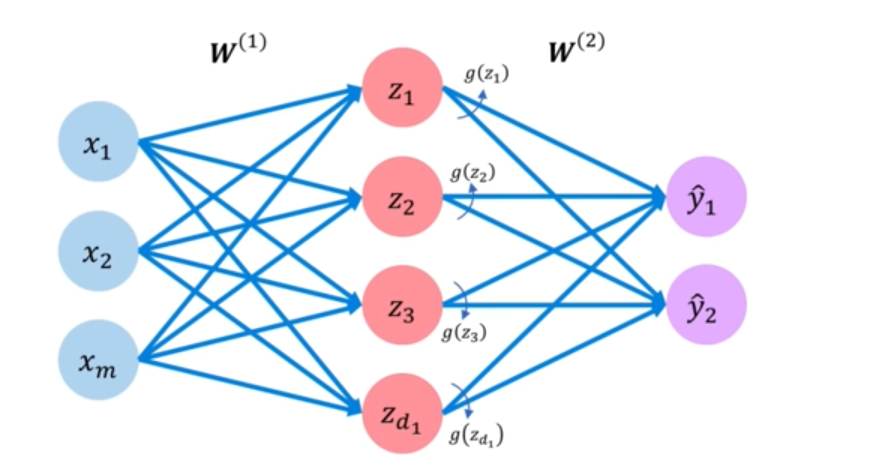
\includegraphics[width=0.5\textheight]{single_layer_nn.png}
	
		\caption{Beispiel eines kleinen Neuronalen Netzes}
		
		\label{im:single_layer_neuralnet}
		%\source{https://www.mathworks.com/help/deeplearning/ref/no\_padding\_no\_strides.gif}
		\source{\cite{introtodeeplearning}}
	\end{figure}

	\noindent Der Parameter $\theta = (w,b)$ setzt sich zusammen aus den Kantengewichten $w_{ij}$ zwischen den Neuronen zweier benachbarter Schichten $l$ und $l+1$, die als Matrizen $W^{(l)}$ geschrieben werden können und den Biases $b^{(l)}$ pro Netz-Schicht. Es gilt also $w = [W^{(1)}, ...], b = [b^{(1)}, ....]$.

	
	\noindent Unter einer Netz-Architektur verstehen wir ein \ac{nn}, bei dem lediglich die Struktur festgelegt ist. Wir sprechen von einem Modell, wenn die einzelnen Parameter durch den Trainingsprozess optimiert und damit bestimmt wurden.
	
	
	
	
	

	
	\subsection{Convolutional Neural Networks}
	\noindent Bei \acfp{cnn} werden sogenannte Convolutional Layers als Netzschichten verwendet. Die Idee besteht darin, dass in einem Bild beispielsweise nahe beieinander gelegene Merkmale im Bild wichtiger sind, als weit auseinander liegende. \\
	
	\noindent Der klassische Aufbau von \acp{cnn} besteht aus mehreren Convolutional Layers, zwischen denen sich sogenannte Pooling-Schichten befinden. Diese sich abwechselnden Schichten werden mit einer klassischen vollständig verknüpften Netzschicht abgeschlossen.\\
	
	\noindent\textbf{Convolutional Layer:}\\
	Bei den Convolutional Layers wird ein Filter über die Eingabe bewegt, siehe \autoref{im:convolution}, woraus eine sogenannte Feature-Map entsteht. Die Gewichte der Filter werden während des Trainings gelernt. Die Größe sowie die Schrittweite (stride), mit der ein Filter in der Raumrichtung verschoben wird, werden vor Beginn des Trainings festgelegt.
	
	\begin{figure}[ht]
		\centering
		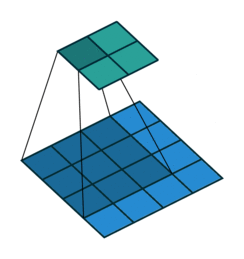
\includegraphics[width=0.1\textheight]{frame_0_delay-1s.png}
		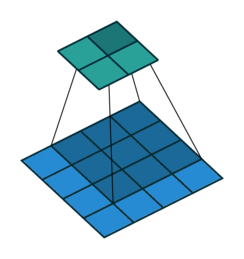
\includegraphics[width=0.1\textheight]{frame_1_delay-1s.png}
		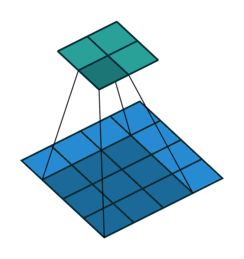
\includegraphics[width=0.1\textheight]{frame_2_delay-1s.png}		
		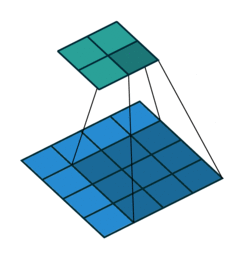
\includegraphics[width=0.1\textheight]{frame_3_delay-1s.png}
		\caption[Funktionsweise einer Convolutional Layer]{Funktionsweise einer Convolutional layer mit Filtergröße $2\times 2$ und Schrittweite $stride=1$}
		
		\label{im:convolution}
		\source{\cite{convolution_matlab}}
	\end{figure}
	

	\noindent\textbf{Pooling Layer:}\\
	\noindent Auf diesen Feature-Maps werden anschließend sogenannte Pooling-O\-pe\-ra\-tio\-nen durchgeführt. Dabei wird beispielsweise ein Average-, Sum- oder Max-Pooling verwendet, um die Dimension einer Feature-Map zu verringern. Wird zum Beispiel für das Max-Pooling ein Fenster der Größe $2 \times 2$ ausgewählt, so wird eine Feature-Map in der Breite und Höhe halbiert, indem das Maximum über diese vier Felder ausgewählt wird.\\
		
	\noindent Ein weiterer Vorteil von \acp{cnn} neben den sehr guten Ergebnissen im Bereich der Bild-Klassifikation besteht darin, dass durch die reduzierte Anzahl an Verbindungen zwischen Neuronen zweier benachbarter Netzschichten die Anzahl der Parameter im Vergleich zu \acp{nn}, die nur aus vollständig verknüpften Schichten bestehen, deutlich reduziert werden kann.
	
	\subsection{Inception-Netze}\label{chapter:inception}
	Bei Inception-Netzen werden nun mehrere Convolution-Operationen nicht nur nacheinander, sondern nebeneinander ausgeführt. Die Ausgaben werden anschließend wieder zusammengefasst (Merging). Diese Art von Schicht bildet das sogenannte Inception-Modul, das für die besondere Struktur der Inception-Netze verantwortlich ist. Dieses wird wieder abwechselnd mit Av\-er\-age- und Max-Pooling-Schichten ausgeführt. Die ursprünglichen Versionen des Inception-Moduls sind in \autoref{inception_modules} abgebildet.
	
	
	
	\begin{figure}
		\centering
		\begin{subfigure}{.5\textwidth}
			\centering
				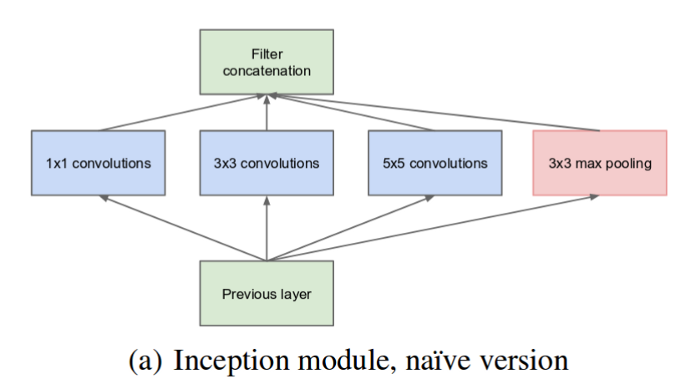
\includegraphics[width=.7\linewidth]{inception_module_naive.png}
			%\caption{Verkehrsschild der Klasse 'Höchstgeschwindigkeit: 50km/h' versehen mit einem 3x3 Sticker und dem Label 'Höchstgeschwindigkeit: 80km/h'}
			
		\end{subfigure}%
		\begin{subfigure}{.5\textwidth}
			\centering
			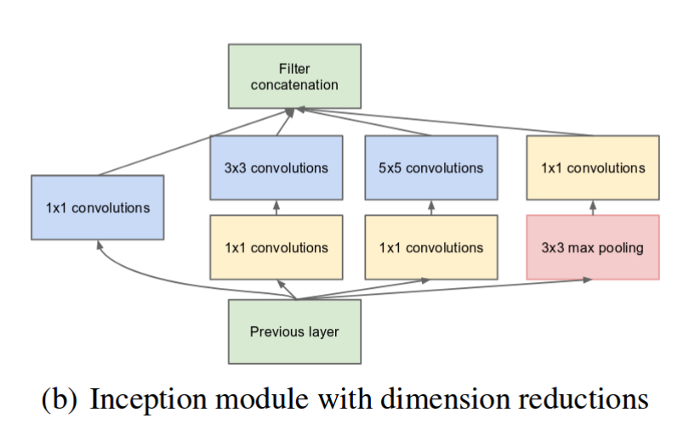
\includegraphics[width=.7\linewidth]{inception_module_advanced.png}
			%\caption{Zugehörige Heatmap bezüglich der Klasse 'Höchstgeschwindigkeit: 80km/h'}
			
		\end{subfigure}
		\caption{Inception-Module}
		\source{\cite{goingdeeperwithconvolutions}}
		
		\label{inception_modules}
	\end{figure}


	\noindent In der zweiten Version der Inception-Netze werden $1\times 1$-Convolutions zur Dimensionsreduktion benutzt, um den Rechenaufwand weiter zu senken.
	Durch das sehr tiefe \ac{nn} entstand auch hier das Problem, dass die Gradienten bei der Backpropagation verschwinden. Um dies zu verhindern, wurden zwei zusätzliche Hilfs-Klassifikatoren an verschiedenen Stellen im \ac{nn} implementiert, die während des Trainings einen Fehler für die Backpropagation beisteuern. Nach dem abgeschlossenen Training werden diese Hilfsklassifikatoren nicht mehr benutzt. Das vollständige \ac{nn} ist in \autoref{inception_v1_structure} dargestellt.
	
	\begin{figure}[ht]
		\centering
		
			\centering
			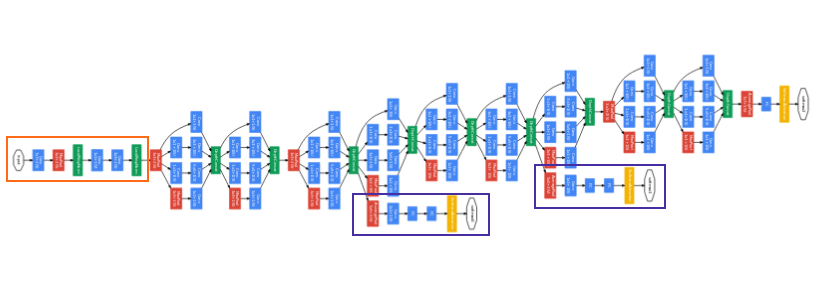
\includegraphics[width=.7\linewidth]{inception_v1_structure.png}
		
		\caption{Inception v1}
		\source{\cite{goingdeeperwithconvolutions}}
		
		\label{inception_v1_structure}
	\end{figure}
	
	\newpage
	\section{Poisoning-Angriffe} \label{chapter_poisoningattacks}
	Während \acp{nn} für schwierige Aufgaben vollautomatisch hochpräzise Entscheidungen treffen, sind diese leider gleichzeitig durch einen Angreifer sehr leicht manipulierbar. Bei Poisoning-Angriffen manipuliert ein Angreifer den Datensatz, der von einem Opfer für das Training eines \ac{nn} verwendet wird. 
	
	
	\noindent Ein Angreifer möchte das Training so beeinflussen, dass die Vorhersagequalität des \ac{nn} im Realbetrieb allgemein verringert ist oder nur bestimmte Eingaben falsch klassifiziert werden.
	Eine Spezialform der letzteren Angriffsmöglichkeit sind sogenannte Backdoor-Poisoning-Angriffe, die eine Hintertür im \ac{nn} implementieren, die im Realbetrieb ausgenutzt werden kann. Dabei werden dann nur diejenigen Bilder einer bestimmten Klasse einer anderen bestimmten Klasse falsch zugeordnet, die einen Auslöser besitzen, der vom \ac{nn} erkannt wird.
	Im Unterschied zu Adversarialen Angriffen, die nach dem Training konstruiert und benutzt werden, finden die \acp{pa} bereits während des Trainings statt, um nach dem Training ausgenutzt zu werden. Nach einem erfolgreichen \ac{pa} arbeitet das Opfer folglich mit einem manipulierten/korrumpierten \ac{nn}.\\
	
	\noindent\textbf{Kenntnisse des Angreifers}: Wir gehen davon aus, dass der Angreifer volle Kenntnis über die Netzwerkarchitektur und Zugriff auf den Datensatz besitzt.\\
	
	\noindent\textbf{Ziel des Angreifers}: Der Angreifer verfolgt das Ziel, während des Trainings
	eine Hintertür im \ac{nn} zu implementieren, die über den Auslöser im Realbetrieb
	genutzt werden kann. Außerdem möchte der Angreifer möglichst wenig Veränderungen am Datensatz durchführen, d.h. nur wenige Datenpunkte sollen manipuliert werden, während der Angriff noch immer erfolgreich funktioniert.
	
	\noindent Ebenfalls wichtig für den Angreifer ist es, dass das \ac{nn} in Abwesenheit eines Auslösers im Realbetrieb möglichst ähnlich gut wie dasselbe Modell, trainiert auf nicht korrumpierten Daten, funktioniert. Andernfalls würde sich bereits während des
	Trainings ein Hinweis darauf ergeben, dass der Datensatz manipuliert ist.
	
	
	
	 
	
	
	\subsection{Standard-Poisoning-Angriffe}
	Bei sogenannten ungerichteten \acfp{pa}, soll durch die Manipulation des Datensatzes die Vorhersagequalität des \ac{nn} abnehmen.\\
	
	\noindent Bei gerichteten \acp{pa} bestimmt der Angreifer eine Start- und Zielklasse und manipuliert den Datensatz so, dass Elemente $x_{source}$ der Klasse $y_{source}$  fälschlicherweise der Klasse $y_{target}$ zugeordnet werden.
	
	\noindent Für die spezielleren Backdoor-\acp{pa} soll eine Hintertür im \ac{nn} $f_\theta$ implementiert werden, die später so ausgenutzt werden kann, dass die oben beschriebene falsche Zuordnung nur in Anwesenheit des Auslösers geschieht. Wir können dies wie folgt formulieren: Sei $f_{\theta,p}$ das manipulierte \ac{nn} und $x_{source,p}$ ein Element der Klasse $y_{source}$, welches im Unterschied zu $x_{source}$ derselben Klasse einen Auslöser enthält. Es soll dann gelten:
	\begin{align*}
		f_{\theta,p}(x_{source,p}) &= y_{target} \\
		f_{\theta,p}(x_{source}) &= y_{source}
	\end{align*}
	
	\noindent Die erste Aussage verlangt, dass ein Element mit einem Auslöser vom manipulierten \ac{nn} der Zielklasse zugeordnet wird.
	Die zweite Aussage fordert, dass die Anwendung des manipulierten \ac{nn} auf den nicht-korrumpierten Datenpunkten keine andere Entscheidung als die Anwendung des nicht manipulierten \ac{nn} zur Folge hat. D.h. in Abwesenheit des Auslösers funktioniert das \ac{nn} wie gewünscht. Dies ist einer der Gründe, weshalb es so schwierig ist, \acp{pa} zu detektieren.
	
	\noindent Um einen solchen Backdoor-Poisoning-Angriff zu implementieren, werden zwei Klassen als Start- und Zielklasse ausgewählt und bei einem bestimmten Anteil der Bilder in der Startklasse wird der Auslöser eingefügt und das Label auf die Zielklasse abgeändert.\\
	
	\noindent Ein Beispiel eines manipulierten Bildes ist in \autoref{im:SPA} abgebildet. Dabei wird ein Auslöser in Form eines Stickers auf dem Verkehrsschild eingefügt und das Label auf die Klasse 80~km/h abgeändert.\\
	
	\noindent In diesem Fall von \acp{pa} spielt es keine Rolle, ob der Angreifer die Netzarchitektur kennt. Wichtig ist nur, dass dieser Zugriff auf den Datensatz besitzt.\\
	
	\begin{figure}[ht]
		\centering
		
\includegraphics[width=0.15\textheight]{1450_poison.jpeg}
		
		
		\caption[Visualisierung des Standard-Angriffs]{Korrumpierte Datenpunkte aus der Start-Klasse~'50~km/h' mit gelb-grünem Sticker und dem Label '80 km/h' der Zielklasse.}
		
		\label{im:SPA}
	\end{figure}
	
	\noindent Wir befassen uns im Folgenden ausschließlich mit Backdoor-Poisoning-An\-grif\-fen
	und sprechen deshalb nur von Standard-Angriffen.\\
	
	
	
	\subsection{Label-konsistente Poisoning-Angriffe}
	Bei den vorherigen Standard-Angriffen war es der Fall, dass das Label und das entsprechende Bild nicht mehr zusammenpassen. Ein händisches Durchsuchen des Datensatzes (wenn auch sehr aufwendig) könnte damit ebenfalls zur Detektion eines Angriffs führen.\\
	Eine deutlich schwieriger zu detektierende Art von \acp{pa} sind sogenannte \acfp{lkpa}, bei denen genau diese Schwachstelle eliminiert ist, d.h. Label und Bild passen wieder zueinander, während der Angriff noch immer erfolgreich funktioniert.
	
	\noindent Auch hier wird wieder ein Auslöser im Bild eingefügt. Auf die Abänderung des Labels wird nun jedoch verzichtet.
	
	\noindent Es ist das Ziel, ein Bild vor dem Anbringen des Auslösers so zu modifizieren, dass es für das menschliche Auge noch immer zur entsprechenden Klasse gehört, für das \ac{nn} aber so schwierig zu klassifizieren ist, dass es sich auf den Auslöser anstatt auf das ursprüngliche Bild verlässt. Im Anschluss wird wieder ein Auslöser eingefügt.
	
	\noindent In \cite{labelconsistent} werden zwei Verfahren vorgestellt, die einzelne Bilder so stören können, dass die Klassifikation erschwert wird. Das erste Verfahren besteht aus einer Einbettung in einen niedrig-dimensionalen Raum, das auch bei Autoencodern \cite{autoencoders} verwendet wird.
	
	\noindent Beim zweiten Verfahren wird ein sogenannter Projektiver Gradienten-Abstieg-Angriff durchgeführt. Dabei wird ein Adversarialer Angriff in leicht abgewandelter Form genutzt, um eine Netzeingabe $x$ zu stören, sodass diese vom \ac{nn} falsch klassifiziert wird, für das menschliche Auge jedoch noch immer zur selben Klasse gehört. Im Unterschied zu Adversarialen Angriffen, bei denen die falschen Klassifikationen nach dem Training eines \ac{nn} stattfinden, sollen die falschen Klassifikationen in diesem Fall bereits während des Trainings des angegriffenen \ac{nn} stattfinden. Diese Störungen lassen sich auch von einem Modell oder sogar einer Architektur auf andere übertragen \cite{szegedy2013intriguing, papernot2016transferability}.
	
	\noindent Zu beachten ist hier, dass für die Manipulation der Datenpunkte ein \ac{nn} benötigt wird. Im Idealfall kennt der Angreifer die Netzarchitektur des Opfers und kann damit dasselbe \ac{nn} für die Implementierung des Angriffs verwenden. Durch die leichte Übertragbarkeit von einem \ac{nn} auf ein anderes, lässt sich dieser Angriff jedoch auch ohne die Kenntnis der vom Opfer ausgewählten Architektur implementieren.

	\noindent Für ein auf nicht manipulierten Daten trainiertes \ac{nn} $f_\theta$ mit Verlustfunktion $\mathcal{L}$ und ein Eingabe-Paar $(x,y)$, wird die modifizierte Version von $x$ konstruiert als
	\begin{equation}
	x_{adv} = \argmax_{||x'-x||_p \leq \varepsilon}{\mathcal{L}(x',y,\theta)},
	\end{equation}
	
	\noindent für $p >1 $ und $\varepsilon > 0$. \\
	
	\noindent Dieses Optimierungsproblem wird mit einem projektiven Gradienten-Verfahren \cite{madry2017towards} wie folgt gelöst:
	
	\noindent Für jeden Datenpunkt $x$ beschreibt $\mathcal{S} \subset \mathbb{R}^d$ die Menge aller zulässigen Störungen. Das Optimierungsproblem wird mit der Iteration
	\begin{equation}
	x^{t+1} = \Pi_{x +\mathcal{S}}(x^t + \alpha sgn(\nabla_x \mathcal{L}(x,y, \theta)))
	\end{equation} für eine Schrittweite $\alpha >0$ und eine Anzahl an Iterationen $n$ gelöst. Dabei bezeichnet $\Pi_{x +\mathcal{S}}(\cdot)$ den Projektionsschritt auf die Menge aller zulässigen Abweichungen von $x$.
	
	\noindent Im Unterschied zu \cite{labelconsistent} ändern wir nur Bilder im Datensatz ab und fügen nicht zusätzlich zum Original $x$ auch $x_{adv}$ hinzu. Damit ändert sich die Anzahl an Datenpunkten durch den Angriff nicht.\\
	
	
	\noindent Für den Auslöser können wir denselben wie im Standard-Fall oder einen schwarz-weißen Sticker der Größe $3\times 3$ benutzen, der in Lesereihenfolge die Farben ssw-sws-wsw (s:schwarz, w:weiß) besitzt. Damit haben wir einen Angriff implementiert,	bei dem Label und Bild wieder zusammenpassen.
	In einem weiteren Schritt ist es möglich, die Sichtbarkeit des Auslösers zu verringern. Dabei werden nun nicht die Pixel-Werte $v_i \in \lbrace 0, 255 \rbrace ^3$ direkt ersetzt, sondern eine Amplitude wird auf allen drei Farbkanälen addiert bzw. subtrahiert. Auf den vorher schwarzen Feldern wird $amp \in\lbrace 16, 32, 64, 128, 256 \rbrace$ addiert und auf den vorher weißen Feldern subtrahiert. Für $amp = 256$ ergibt sich der Fall, bei dem die Pixel-Werte durch schwarze bzw. weiße Pixel getauscht werden. Im entsprechenden Paper \cite{labelconsistent} wird auch ein Auslöser eingefügt, bei dem	sich jeweils ein solcher Sticker in jeder Bildecke befindet. 
	
	
	\begin{figure}[ht]
		\centering
		
\includegraphics[width=0.1\textheight]{32_1corner_infty300.jpeg}
		
\includegraphics[width=0.1\textheight]{64_1_coner:infty300.jpeg}
		
\includegraphics[width=0.1\textheight]{255_1corner_infty300.jpeg}		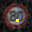
\includegraphics[width=0.1\textheight]{sticker_infty300.jpeg}
		\caption[Korrumpierte Datenpunkte für Label-konsistente Poisoning-Angriffe]{Korrumpierte Datenpunkte mit Amplitudensticker unten rechts für $amp=32,64,255$ und dem Standard-Auslöser (rechts).}
		
		\label{im:LCPA}
	\end{figure}


	
	
	\subsection{Bewertung von Poisoning-Angriffen}
	Um verschiedene \acp{pa} miteinander vergleichen zu können, benötigen wir ein Maß dafür, wie erfolgreich ein bestimmter Angriff funktioniert. 
	
	\noindent Für den Fall der Standard-Angriffe wird der gewählte Auslöser bei allen Bildern der Startklasse im Testdatensatz eingefügt und der Anteil an Bildern bestimmt, die aus der Startklasse stammen und in Anwesenheit des Auslösers der Zielklasse zugeordnet werden.
	
	\noindent Dieser Anteil definiert die sogenannte \acf{aer}. Für die \\ \noindent \acp{lkpa} werden im Test-Datensatz alle Bilder mit
	dem entsprechenden Auslöser versehen und es kann eine \ac{aer} pro Klasse
	berechnet werden. Es ist zu beachten, dass für Angriffe, die mit einer reduzierten
	Amplitudenstärke durchgeführt werden, die Bilder im Test-Datensatz dennoch mit
	Auslösern mit voller Amplitudenstärke versehen werden. Wir bewerten die Qualität
	eines \ac{lkpa} über die \ac{maer} über alle Klassen außer der Zielklasse.
 	
	
	\section{Detektionsverfahren}
	In diesem Kapitel beschäftigen wir uns mit gängigen Methoden zur Detektion von \acp{pa} und geben am Ende einen kurzen Ausblick auf die Idee für einen neuen Ansatz. Wir wollen beide Arten von \acp{pa} erfolgreich detektieren. 
	
	\subsection{Detektion eines Poisoning-Angriffs}
	
	Es muss zunächst diejenige Klasse bestimmt werden, für die der Verdacht besteht, dass über diese ein \ac{pa} durchgeführt wurde.
	
	\noindent Anschließend kommt ein Clustering-Algorithmus zum Einsatz, der die Daten im Idealfall in in zwei Cluster aus sauberen Datenpunkten und korrumpierten Datenpunkten aufteilt.\\
	
	\noindent Zur Bestimmung, ob eine Klasse korrumpierte Daten enthält, kann das Ergebnis
	des Clusterings mit den folgenden Methoden untersucht werden:\\
	
	\noindent \textbf{Vergleich der relativen Größe:} Eine Möglichkeit, korrumpierte Datenpunkte
	zu erkennen, ist der Vergleich der relativen Größen der beiden Cluster. Laut \cite{AC}
	liegt die relative Größe bei nicht korrumpierten Klassen bei ca. 50 Prozent. Bei korrumpierten Daten und einem erfolgreichen Clustering würde die relative Größe dann dem prozentualen Anteil an korrumpierten Datenpunkten entsprechen.\\
	
	\noindent \textbf{Silhouettenkoeffizient:} Eine weitere Möglichkeit besteht darin, die Qualität
	des Clusterings mit Hilfe des Silhouette-Koeffizienten zu beschreiben. Dieser gibt
	an, wie gut ein Clustering zu den gegebenen Datenpunkten mit den entsprechenden Labeln passt und ist wie folgt definiert: Sei das Ergebnis eines Clustering-Algorithmus mit verschiedenen Clustern gegeben. Zu einer Beobachtung $x$ im Cluster $A$ wird die Silhouette \begin{equation}
		s(x) = \frac{d(B,x)-d(A,x)}{\max\lbrace d(A,x), d(B,x) \rbrace}
	\end{equation} definiert, wobei $d(A,x)  = \frac{1}{n_A -1}\sum_{a \in A, a \neq x}{d(a,x)}$ dem mittleren Abstand einer Beobachtung innerhalb dieses Clusters zu allen anderen Beobachtungen dieser Klasse entspricht.
	Dabei steht $n_A$ für die Anzahl der Beobachtungen in Cluster A. $d(B,x) = \min_{C \neq A}d(C,x)$ beschreibt die Distanz von $x$ zum nächstgelegenen Cluster B. Der Silhouetten-Koeffizient $SC$ ist nun definiert als
	\begin{equation}
	SC = \max_k \tilde{s}(k),
	\end{equation}
	wobei $\tilde{s}(k)$ der Mittelwert der Silhoutten aller Datenpunkte im gesamten Datensatz unter Verwendung von k Clustern ist. Damit ist der Silhouttenkoeffizient ein Maß dafür, wie gut ein Clustering für eine vorher fixierte Clusteranzahl $k$ zum Datensatz passt.\\
	
	\noindent \textbf{Exklusives Retraining:} Beim exklusiven Retraining wird das \ac{nn}
	von Grund auf neu trainiert. Das oder die verdächtigen Cluster werden beim
	erneuten Training nicht verwendet. Mithilfe des neu trainierten \ac{nn} werden dann anschließend die vorenthaltenen, verdächtigen Cluster klassifiziert.
	Falls das Cluster Aktivierungen von Datenpunkten enthält, die zum Label des Datenpunktes gehören, erwarten wir, dass die Vorhersage des \ac{nn} mit
	dem Label übereinstimmen. Gehören die Aktivierungen eines Datenpunktes im
	verdächtigen Cluster jedoch zu einer anderen Klasse als die durch das Label
	angedeutete Klasse, so sollte das \ac{nn} den Datenpunkt einer anderen Klasse zuordnen. Um nun zu entscheiden, ob ein verdächtiges Cluster korrumpiert
	oder nicht korrumpiert ist, wird wie folgt vorgegangen: Sei $l$ die Anzahl an Vorhersagen, die zum Label des Datenpunktes passen. Sei $p$ die größte Anzahl an
	Vorhersagen, die für eine weitere Klasse $C$ sprechen, wobei $C$ nicht die Klasse mit den Labeln des zu untersuchenden Clusters ist. Der Quotient $\frac{l}{p}$ gibt
	dann an, ob das Cluster korrumpiert ist oder nicht: Es wird ein Schwellenwert
	$T > 0$ gesetzt. Gilt $\frac{l}{p} < T$, wurden mehr Datenpunkte einer anderen Klasse zugeordnet und das Cluster wird als korrumpiert deklariert. Umgekehrt wird das
	verdächtige Cluster im Fall von $\frac{l}{p} > T$ als nicht korrumpiert eingestuft.
	
	
	
	
	
	
	
	\subsection{$k$Means-Clustering}\label{chapter:kMeans}
	Das $k$Means-Clustering gehört zu den unüberwachten Clustering-Verfahren. Bei diesen Verfahren existieren keine Datenpaare, die für eine Art Training verwendet werden können. In der ursprünglichen Formulierung von $k$Means sind $n$ Datenpunkte $x_1,...,x_n \in \mathbb{R}^d$ und $k \in \mathbb{Z}_{>0}$ gegeben. Die Datenpunkte sollen so auf die einzelnen Cluster verteilt werden, dass die Distanzen innerhalb eines Clusters zum Cluster-Zentrum minimal sind. Für das $k$Means-Clustering müssen wir im Vorfeld eine Clusteranzahl $k$ fixieren und die Mittelpunkte der k Cluster initialisieren.\\
	
	\noindent In Lloyd's Formulierung \cite{lloyd1982least} wird mit einer gleich-verteilten zufälligen Initialisierung von $k$ Cluster-Zentren begonnen. Jeder Punkt im Datensatz wird anschließend dem nächstgelegenen Cluster-Zentrum zugeordnet. Für jedes Cluster wird anschließend ein neues Zentrum als Mittelwert berechnet.
	
	\noindent Diese beiden Schritte aus Zuordnung und Mittelpunktberechnung werden so lange wiederholt, bis sich die Cluster-Zentren nicht mehr ändern oder eine maximale Iterationszahl erreicht ist.
	
	\noindent Eine Variation des $k$Means-Algorithmus, der sowohl die Laufzeit als auch die Genauigkeit verbessert, ist der sogenannte $k$Means$++$-Algorithmus \cite{kmeans++}. Dabei wird die Initialisierung in abgewandelter Form durchgeführt. Nach gleichverteilter, zufälliger Bestimmung des ersten Cluster-Zentrums werden die übrigen $k-1$ Zentren wie folgt gewählt:
	Die Wahl erfolgt proportional zur maximalen quadratischen Distanz zu allen vorher bestimmten Cluster-Zentren. Damit sind die Zentren so über den Datensatz verteilt, dass sie maximal weit auseinander liegen.\\
	
	\noindent Anschließend werden die im kMeans-Algorithmus üblichen Schritte aus Distanzberechnung und Mittelwert-Berechnung wiederholt.\\
	
	\noindent Das $k$Means$++$-Clustering ist nochmals in Algorithmus \autoref{alg:kmeans} dargestellt.
	
	\begin{algorithm}[h]
		\hspace*{\algorithmicindent} \textbf{Input: } Data points $\mathcal{X} = \lbrace x_1,...,x_n \rbrace$, Number of Clusters $k$, distance function $d$, where $D(x)$ is the minimal distance $d(x,c)$, where $c$ are the already choosen cluster centers.		\newline
		\hspace*{\algorithmicindent} \textbf{Output: } $k$ Cluster centers $\mathcal{C}=\lbrace c_1,...,c_k\rbrace$. 
		
		\caption{kMeans-Algorithmus}
		\label{alg:kmeans}
		
		\begin{algorithmic}
			\STATE{Arbitrarily choose $k$ initial centers $\mathcal{C}={c_1,...,c_k}$}
			\REPEAT
			\STATE{For each $i \in \lbrace 1,...,k \rbrace$, set the cluster $C_i$ to be the set of points in $\mathcal{X}$ that are closer to $c_i$ than they are to $c_j$ for all $j\neq i$.}
			\STATE{For each $i \in \lbrace 1,...,k \rbrace$, set $c_i$ to be the centere of mass of all points in $C_i: c_i = \frac{1}{|C_i|}\sum_{x \in C_i}{x}$.}
			\UNTIL{convergence}
		\end{algorithmic}
		
		
	\end{algorithm}
	
	\noindent Die Initialisierung für den kMeans++-Algorithmus ist in Algorithmus \autoref{alg:kmeans++_init} notiert.
	\begin{algorithm}
		\hspace*{\algorithmicindent} \textbf{Input: } Data points $\mathcal{X} = \lbrace x_1,...,x_n \rbrace$, Number of Clusters $k$.		\newline
		\hspace*{\algorithmicindent} \textbf{Output: } $k$ Clusters. 
		\caption{kMeans++-Initalisierung}
		\label{alg:kmeans++_init}
		
		
		\begin{algorithmic}
			
			\STATE{Choose an initial center $c_1$ uniformly at random from $\mathcal{X}$.}
			\REPEAT
			\STATE{Choose the next center $c_i$, selecting $c_i = x' \in \mathcal{X}$ with probability $\frac{D(x')^2}{\sum_{x\in\mathcal{X}}{D(x)^2}}$.}
			
			\UNTIL{we have choosen a total of $k$ centers}
		\end{algorithmic}
	\end{algorithm}	
	
	\noindent Es bleibt also die Bestimmung des Wertes $k$.
	Dafür benutzen wir die Spektralzerlegung, die wir im nächsten Abschnitt vorstellen.
	
	\newpage
	\subsection{Spektrales Clustering/Spektrale Zerlegung}
	%Wir folgen \cite{spectralClustering_tut} und \cite{unmaskingCH}.
	
	\noindent Wir gehen davon aus, dass uns ein metrischer Raum $(X,d)$ gegeben ist, wobei $X = \lbrace x_i, ..., x_n \rbrace$ gilt.
	In \cite{spectralClustering_tut} wird der metrische Raum als Graph ${G=(V,E)}$ interpretiert. Damit wird aus dem Clustering-Problem ein äquivalentes Partitionierungsproblem in $k$ Partitionen:
	\begin{center}
		\textit{Finde eine Partitionierung des Graphen $G$, sodass die Kantengewichte \\innerhalb eines Clusters minimal sind.}
	\end{center}
	\noindent Um aus dem metrischen Raum $(X,d)$ einen Graphen zu erhalten, müssen zwischen den Knoten des Graphen Kanten definiert werden. Dafür existieren die folgenden drei Möglichkeiten:
	
	\begin{itemize}
		\item $\varepsilon$-Nachbarschaftsgraph: Hier wird eine Kante zwischen zwei Knoten $u$ und $v$ gesetzt, falls $d(u,v) \leq \varepsilon$ für $\varepsilon > 0$ gilt.
		\item $kNN$-Graph: Hier wird eine Kante zwischen zwei Knoten $u$ und $v$ gesetzt, falls $v$ unter den $k$ vielen Knoten ist, die am nächsten an $u$ liegen.
		\item Vollständiger Graph: Hier wird eine Kante zwischen allen Knoten im Graphen gesetzt.
	\end{itemize}
	
	\noindent Analog zu \cite{unmaskingCH} entscheiden wir uns für einen $kNN$-Graphen mit $k~=~10$. Die Adjazenzmatrix $A = (a_{ij})_{ij}$ eines Graphen $G$ ist definiert durch
	\begin{equation}
	a_{ij} = \begin{cases}
	1, \text{ falls  } u \text{ und } v \text{ verbunden sind,}\\
	0, \text{ sonst.}
	\end{cases}
	\end{equation}
	
	
	
	\noindent Ausgehend davon lässt sich die zu einem Graphen $G$ gehörige Laplace-Matrix definieren:
	
	\begin{definition}[Laplace-Matrix]
		Sei $G=(V,E)$ ein Graph mit Adjazenzmatrix $A$. Sei $D = (d_{ij})_{ij}$ eine Diagonalmatrix mit $d_{i} = \sum_{j=1}^n{a_{ij}}$. Sei $L=D-A$ die \emph{nicht normalisierte Laplace-Matrix}. Dann lässt sich die symmetrische und normalisierte Laplace-Matrix $L_{sym}$ definieren als
		\begin{equation}
		L_{sym} = D^{-1/2}LD^{-1/2}.
		\end{equation}
	\end{definition}
	
	
	\noindent Wir zitieren das folgende Resultat:
	
	\begin{theorem}[Anzahl an zusammenhängenden Komponenten und Spektrum von $L_{sym}$ \cite{spectralClustering_tut}]
		Sei $G$ ein ungerichteter Graph mit nicht-negativen Gewichten. Dann gibt die Vielfachheit der Eigenwerte $0$ von $L_{sym}$ die Anzahl an zusammenhängenden Komponenten $A_1,..., A_k$ an.
	\end{theorem}
	
	\noindent Damit können wir also die optimale Clusteranzahl $k$ durch eine spektrale Zerlegung bestimmen und anschließend das Clustering durchführen.
	
	\subsection{Clustering-Verfahren}
	Alle in dieser Arbeit vorgestellten Detektionsverfahren basieren auf der Idee, die Daten in einen korrumpierten und einen unkorrumpierten Anteil aufzuteilen. Dafür wird jeweils ein Clusteringverfahren verwendet, das unterschiedliche Repräsentationen der Daten benutzt. 
	
	\begin{remark}
		Um von einer verdächtigen Klasse in einem Datensatz sprechen zu können, muss auch diese erst einmal identifiziert werden.
		In \cite{imagenet_unhansed_v1} Kapitel '2.3. Fisher Discriminant Analysis for Clever Hans
		identification' wird ein Verfahren vorgestellt, mit dem verdächtige Klassen identifiziert werden können. Für diese würde man anschließend das Heatmap-Clustering durchführen. Wir gehen im Folgenden davon aus, dass wir die verdächtige Klasse bereits identifiziert haben.
	\end{remark}

	\noindent Im Folgenden stellen wir drei solcher Clustering-Verfahren vor.
	
	\subsubsection{Clustering auf den Rohdaten}
	Der einfachste Ansatz, um korrumpierte Datenpunkte zu erkennen, ist ein $k$Means-Clustering, das direkt (bzw. nach einer Dimensionsreduktion) auf den Eingabedaten einer Klasse durchgeführt wird. 
	
	\subsubsection{Activation-Clustering}
	
	
	Das \acf{ac} als Verteidigungsstrategie basiert auf der Annahme, dass bestimmte Schichten innerhalb des \ac{nn} die Entscheidung, dass ein Bild mit einem Auslöser falsch klassifiziert wird, sehr gut codieren. Für die Detektion der Hintertüren im Datensatz sollen nun genau diese Aktivierungen als Grundlage für das $k$Means-Clustering herangezogen werden.\\
	Das \ac{ac} wird erstmalig in \cite{AC} vorgestellt und nutzt aufgrund experimenteller Untersuchungen stets die Aktivierungen der vorletzten Netzschicht. Eine Kombination von Aktivierungen mehrerer Schichten wäre ebenfalls denkbar.
	
	
	\begin{comment}
	
	\begin{remark}
		Das Activation Clustering benutzt die Idee, dass innerhalb einer Klasse bezüglich unterschiedlicher Aktivierungen klassifiziert werden kann. Beim CLPA funktioniert das nicht mehr, denn: Hier passen jetzt auch die Aktivierungen der korrumpierten Bilder zur entsprechenden/untersuchten Klasse. Es ist also zu erwarten, dass das AC für CLPA nicht funktioniert.
	\end{remark}
		
	\end{comment}
	
	
	

	
	\subsubsection{Heatmap-Clustering} \label{chapter:algorithm}
	In diesem Abschnitt stellen wir das \acf{hc} vor, mit dem \acp{pa} detektiert werden können. Dieses von uns neu entwickelte Verfahren stellt den Kern dieser Arbeit dar und funktioniert wie im Folgenden dargestellt.\\
	
	\noindent \textbf{Grundsätzliches Vorgehen}\\
	\noindent Die Idee besteht darin, ein $k$Means-Clustering auf einer Klasse durchzuführen, die in dem Sinne für verdächtig gehalten wird, dass innerhalb dieser Klasse Datenpunkte eingefügt wurden, die nicht zum ursprünglichen Datensatz gehören und eine Hintertür im \ac{nn} implementieren sollen.\\
	
	\noindent Wichtig für das Clustering sind hierbei die Repräsentation der Daten, auf denen geclustert wird, sowie die Metriken, die eine Distanz und damit auch einen Mittelwertbegriff für mehrere Datenpunkte definieren.
	
	\noindent Als Repräsentation benutzen wir die Heatmaps, die mit der \ac{lrp}, wie in \autoref{chapter_lrp} beschrieben, erzeugt werden.\\
	
	\noindent Dieses Verfahren besteht also darin, eine Spektrale Relevanz Analyse \cite{unmaskingCH} durchzuführen, die aus einem Spektralen Clustering auf Heatmaps durchgeführt wird, die mit der \ac{lrp} berechnet wurden.\\
	
	\noindent Wir können die einzelnen Schritte des Verfahrens wie folgt zusammenfassen:	
	\begin{itemize}
		\item Berechnung der Heatmaps mithilfe der \ac{lrp} (vgl. \autoref{chapter_lrp})
		\item Berechnung einer Distanzmatrix 
		\item Spektrale Zerlegung (vgl. \autoref{chapter:kMeans})
		\\ (Bestimmung der verschiedenen Cluster innerhalb einer Klasse)
		\item $k$Means-Clustering zur Bestimmung der korrumpierten Datenpunkte (vgl. \autoref{chapter:kMeans})
	\end{itemize}
	
	
	\noindent \textbf{Verwendete Distanzen und  Approximationen}\\
	\noindent Bisher sind wir nicht näher auf die Distanz zwischen zwei verschiedenen Heatmaps eingegangen. Um die Struktur innerhalb einer Klasse zu analysieren, benötigen wir jedoch eine Metrik.
	
	\noindent Die naheliegendste Möglichkeit von einer Distanz zwischen zwei Heatmaps zu sprechen, ist vermutlich eine $L^p$-Distanz, bei der die Pixelwerte die einzelnen Komponenten darstellen. 
	
	\noindent Eine andere Idee ist die Verwendung eines Distanzbegriffs, der im Unterschied zur $L^p$-Distanz auch rotations- und translationsinvariant ist. Die Vermutung ist hier, dass wir dadurch einen Distanzbegriff erhalten, der eher mit der menschlichen Wahrnehmung übereinstimmt und sich besser für das Clustering eignet. Dafür verwenden wir die in \autoref{ot} vorgestellte \ac{gwd} und berechnen eine Approximation wie in  \autoref{chapter:GW_regularized} angegeben.
	  
	
	\begin{comment}
		content...
	
	Wie in \cite{imagenet_unhansed_v1} summieren wir über die Farbkanäle, um einen einzelnen Relevanzwert pro Pixelpunkt zu erhalten. Wir benötigen also eine Metrik zur Berechnung der Distanz zwischen 32x32 großen Heatmaps.\\
	Wir normalisieren die Relevanzen zusätzlich auf das Intervall $[0,1]$.\\
	Die Wahl der Pixel mit 99 Prozent der Gesamtmasse und anschließende Normalisierung wird vermutlich durchgeführt, um die Bedingung \autoref{eq:bed_mmspaces} zu erhalten und auch deshalb oder eher nur um zwei verschiedene metrsiche Maßräume zu erhalten, d.h. für zwei MMR $X_1=(X_1,d_1,\mu_1)$ und $X_2=(X_2,d_2,\mu_2)$ gilt $(X_1,d_1) \neq (X_2,d_2)$. Erhalten wir dadurch die Translationsinvarianz?\\
	%TODO: Das sollte vermultich eher an das Ende von OPTIMAL Transport
	\end{comment}
	

	
	
	
	\subsection{Bewertung von Detektionsverfahren}\label{chapter:detectionevaluation}
	
	Die Bewertung eines Detektionsverfahrens entspricht der Bewertung des zugrundeliegenden Clustering-Verfahrens.
	Für die Implementierung der \acp{pa} wie in \autoref{chapter_poisoningattacks} beschrieben, ergeben sich innerhalb der verdächtigen Klassen genau zwei Cluster. Wir führen deshalb ein $k$Means-Clustering für $k=2$ Cluster durch. Das $k$Means-Clustering weist die einzelnen Datenpunkte der unkorrumpierten oder korrumpierten Klasse zu. Wir bezeichnen den korrumpierten Fall als positives Ergebnis und den unkorrumpierten Fall als negatives Ergebnis.\\
	
	\noindent Für ein gegebenes Clustering und unter Kenntnis der Grundwahrheiten bezüglich der Manipulation, können wir die folgenden Größen definieren:\\
	
	\noindent $\boldsymbol{TP}$ (true positives) steht für die Anzahl an positiven Zuordnungen bei positiver Grundwahrheit, d.h. ein korrumpiertes Bild wird richtigerweise als korrumpiert deklariert.\\
	
	\noindent $\boldsymbol{TN}$ (true negatives) beschreibt die Anzahl an negativen Zuordnungen bei negativer Grundwahrheit.\\

	\noindent Für die falschen Zuordnungen zählen wir mit $\boldsymbol{FP}$ (false positives) die Anzahl der positiven Zuordnungen, obwohl die Grundwahrheit negativ ist.\\
	
	\noindent Umgekehrt steht $\boldsymbol{FN}$ (false negatives) für die Anzahl an negativen Zuordnungen bei positiver Grundwahrheit.\\
	 
	\noindent Damit lassen sich für genau zwei gesuchte Cluster die folgenden Größen definieren, um die Qualität des Clusterings zu beschreiben:
	
	\noindent Die Genauigkeit (accuracy) der Vorhersage ist definiert durch den Quotienten \begin{equation}
		ACC = \frac{TP +TN}{TP + FN + FP +TN}.
	\end{equation} 
	
	\noindent Um zu beschreiben, wie gut korrumpierte Datenpunkte als korrumpiert erkannt werden, verwenden wir die True Positive Rate 
	\begin{equation}
		TPR = \frac{TP}{TP + FN}.
	\end{equation}
	
	\noindent Analog beschreibt die True Negative Rate 
	\begin{equation}
		TNR = \frac{TN}{TN +FP},
	\end{equation} wie gut das Clustering nicht korrumpierte Datenpunkte als nicht korrumpiert erkennt.
	
	


	
	
	\section{Erklärbare Künstliche Intelligenz}
	\label{chapter_xai}
	
	Unter dem Begriff Erklärbare Künstliche Intelligenz werden Methoden zusammengefasst, die einzelne Modelle oder Entscheidungen eines Modells erklären.\\
	
	\noindent Bei unkritischen Anwendungen wie beispielsweise Produkt- und Filmempfehlungen oder maschineller Übersetzung spielt die Frage, wie das \ac{ki}-System zu einer Entscheidung bzw. Ausgabe gekommen ist, keine entscheidende Rolle. Anders sieht es jedoch bei Anwendungen in sicherheitskritischen Bereichen aus. Hier kann es sein, dass die Erklärung für das Zustandekommen einer Entscheidung genauso wichtig wie die Entscheidung selbst\cite{LRP_DNN} ist. Zudem sollte die verwendeten Modelle auch nicht diskriminierend sein und durch die Datenschutzgrundverordnung (DSGVO) besitzt der Nutzer sogar ein Recht auf Erklärbarkeit.\\
	
	\noindent Es wird zwischen sogenannten White-Box- und Black-Box-Modellen unterschieden. Bei White-Box-Modellen lassen sich die algorithmischen Zusammenhänge sehr leicht nachvollziehen und die getroffenen Entscheidungen sind daher selbsterklärend. Dazu gehören beispielsweise Lineare Modelle, Regelsysteme oder Entscheidungsbäume.\\
	
	\noindent Bei Black-Box-Modellen wie \acp{nn} ist es aufgrund ihrer Verflechtung und Vielschichtigkeit in der Regel nicht mehr möglich, die innere Funktionsweise des Modells nachzuvollziehen. Zumindest für die Erklärung von Einzelentscheidungen (lokale Erklärbarkeit) können dann jedoch zusätzliche Erklärungswerkzeuge eingesetzt werden, um nachträglich die Nachvollziehbarkeit zu erhöhen. \\
	
	\noindent Lipton \cite{lipton} führt eine grundsätzliche Begriffserklärung ein. Dabei wird zwischen den Begriffen Transparenz (oder Interpretierbarkeit) und Erklärbarkeit wie folgt unterschieden \cite{kistudie}.\\
	
	
	\noindent \textbf{Transparenz: }\\
	Transparenz wird als eine Modelleigenschaft verstanden. Ist die Transparenz eines Modells
	gegeben, so ist es unter der Annahme nachvollziehbarer Eingangsgrößen selbsterklärend. Die Eigenschaft der	Transparenz wird in \cite{lipton} auf drei verschiedenen Ebenen definiert. Dabei wird zwischen Simulierbarkeit (Ebene des gesamten Modells), Unterteilbarkeit (Ebene einzelner Modellkomponenten, z.B. Parameter) und Algorithmischer Transparenz unterschieden. Es wird von einer hierarchischen Abhängigkeit ausgegangen, sodass die Simulierbarkeit eines Systems dessen Unterteilbarkeit und dessen algorithmische Transparenz	impliziert. 
	
	\noindent Ein System heißt simulierbar, wenn
	auch eine Person die Entscheidungen des zugrundeliegenden Algorithmus in angemessener
	Zeit nachvollziehen kann, indem sie alle notwendigen  Berechnungsschritte selbst ausführt \cite{lipton}.
	
	\noindent In einem unterteilbaren System können die einzelnen Komponenten (Eingangsdaten, Parameter,
	Modellebenen, Berechnungen etc.) mit einer intuitiven
	Beschreibung versehen werden, sodass ihre Funktionen
	im Gesamtsystem nachvollziehbar sind.\\
	Algorithmische Transparenz bezieht sich auf den eigentlichen Lernprozess eines Modells. Hierbei kommt es darauf an, ob nachvollzogen werden kann, wie ein Modell im Detail erzeugt wird \cite{kistudie}.\\

	\noindent \textbf{Erklärbarkeit: }\\
	Für diverse Modelle wie beispielsweise \acp{nn} lässt sich Transparenz aufgrund ihrer Komplexität nicht erreichen. Somit sind diese nicht selbsterklärend. Eine Möglichkeit, das Verständnis solcher Modelle trotzdem zu verbessern, bietet das Konzept der Erklärbarkeit. Grundsätzlich wird zwischen zwei Arten von Erklärungen unterschieden \cite{kistudie}:
	
	\begin{itemize}
		\item Erklärungen von Einzelentscheidungen, die dabei helfen, individuelle, datenbezogene Entscheidungen konkret nachzuvollziehen (lokale Erklärbarkeit oder Datenerklärbarkeit).
		\item Erklärungen von Modellen,	die dabei helfen, Wirkzusammenhänge von \ac{ki}-Modellen zu begreifen (sogenannte globale Erklärbarkeit
		oder Modellerklärbarkeit), z. B. lineare oder allgemein funktionale Zusammenhänge zwischen Eingangs- und Ausgangsgrößen.
	\end{itemize}
	
	\noindent In den folgenden beiden Abschnitten stellen wir einige der bekanntesten Methoden aus beiden Bereichen vor.

	\subsection{Lokale Methoden}\label{chapter:localmethods}
	
	\noindent Mithilfe sogenannter \textbf{Attributionsmethoden} wird der
	negative oder positive Einfluss von Teilen oder Bereichen der Eingabe eines \ac{ki}-Modells auf dessen Ausgabe	betrachtet. Dieser Gruppe können z.B. die folgenden konkreten Methoden zugeordnet
	werden: Sensitivitätsanalyse, \ac{lrp} (s. \autoref{chapter_lrp}), DeepLIFT, Integrated Gradients, Grad-CAM, Guided Backpropagation und
	Deconvolution.\\
	
	
	\noindent Bei \textbf{SHAP} handelt es sich um einen Ansatz aus der Spieltheorie. Dabei wird jedes Feature bzw. jede Eingabe bezüglich eines konkreten  Klassifikationsergebnisses gewichtet. Diese 
	Gewichte werden auch als \textit{Shapley Values} bezeichnet. Die Idee dahinter ist, dass alle möglichen Kombinationen von Features betrachtet werden, um die Wichtigkeit eines einzelnen Features zu bestimmen. Jedem Eingabefeature wird so ein positiver oder negativer Wert 
	zugeordnet, der den Einfluss des einzelnen Features auf das Ergebnis angibt. Die Methode kann genutzt werden, um Entscheidungserklärungen zu generieren. TreeSHAP ist eine Variante von SHAP, die besonders effizient auf baumbasierte Modelle angewendet werden kann.\\
	

	
	\noindent Bei der Erstellung von \textbf{Surrogat-Modellen} geht es darum, auf Grundlage eines Black-Box-Modells ein zweites Modell zu erstellen, z. B. ein lineares Modell oder einen Entscheidungsbaum, das besser nachvollziehbar ist und zur Erklärung der Entscheidungen genutzt werden kann. Aufbauend auf den Ein- und Ausgaben des ursprünglichen Modells, wird die Vorhersagefunktion des Surrogat-Modells abgeleitet. So können Regeln aus trainierten 
	\acp{nn} extrahiert und, darauf aufbauend, nachvollziehbare Entscheidungsbäume erstellt werden. Insbesondere für Bilddaten ist die Erstellung derartiger Bäume nicht trivial.\\
	
	\noindent Die Grundidee von \textbf{LIME} ist das Erlernen eines lokal approximierten, interpretierbaren Modells für ein konkretes 
	Klassifikations-­ oder Regressionsergebnis. Dadurch 
	kann mithilfe eines einfacheren, oft linearen Modells ein konkretes Ergebnis nachvollzogen werden, obwohl das ursprüngliche Modell nur schwer nachvollziehbar ist. LIME „sampelt“ mehrere Ergebnisse (bzw. Entscheidungen) und gewichtet diese entsprechend ihrer Nähe zum zu erklärenden Ergebnis. Auf dieser Basis kann ein lokales Modell entwickelt werden, das mit den betrachteten Samples gut funktioniert und nachvollziehbar ist.\\
	
	\noindent Weitere Bereiche für Lokale Methoden sind in \cite{kistudie} angegeben.
	

	
	\subsection{Globale Methoden}
	
	Während die bisher vorgestellten Methoden den Fokus auf die Erklärbarkeit von Einzelentscheidungen eines Modells richten, befassen sich die Methoden in diesem
	Abschnitt damit, das Modell als Ganzes zu verstehen. Diese Methoden versuchen allgemeine
	Muster aus dem Klassifizierungsverhalten des Modells zu extrahieren, indem einzelne Entscheidungen zusammengefasst und anschließend analysiert werden \cite{samek2019towards}.\\
	In diesem Abschnitt werden die Methoden Spectral Relevance Analysis (SpRAy),
	Feature Visualization, Network Dissection und Testing with Concept Activation Vectors (TCAV) vorgestellt.\\
	
	\noindent \textbf{Spectral Relevance Analysis (SpRAy)} ist eine Weiterentwicklung der \ac{lrp}. Mit
	dieser Methode werden zunächst Relevanzklassen für interessante Datensätze und
	Objektklassen über die \ac{lrp} bestimmt. Die Ergebnisse werden in Heatmaps dargestellt
	und anschließend über eine Spektralanalyse geclustert. Jedes Cluster entspricht einer
	durch das Modell erlernten Vorhersagestrategie. Auf diese Weise werden die verwendeten Vorhersagestrategien für Objekte aus den erzeugten Clustern ermittelt\cite{unmaskingCH}. Mit dieser Methode lassen sich Schwachstellen in Datensätzen und Modellen erkennen. Es wird zum Beispiel erkannt, wenn eine Klassifizierung aufgrund der Metadaten eines Bildes vorgenommen wurde.\\
	
	
	\noindent \textbf{Feature Visualization} arbeitet sich ebenso schrittweise durch das \ac{nn},
	um zu verstehen, wie das Modell sein Verständnis über das Ausgangsbild erstellt.
	Es wird erkundet, welche Eingabedaten für ein bestimmtes Verhalten (zum Beispiel eine Neuronen-Aktivierung oder die endgültige Ausgabe) verantwortlich sind. Über eine Optimierung wird ein Verständnis darüber aufgebaut, wonach ein Modell sucht. Dies können beispielsweise Neuronen, Kanäle, Schichten oder
	Klassenwahrscheinlichkeiten sein \cite{feature_vis}.\\
	
	
	\noindent \textbf{Network Dissection} ermöglicht zu verstehen, was in den einzelnen Schichten eines \ac{cnn} geschieht. Die Methode gleicht die Ausgabe jeder Netzschicht mit visuellen semantischen Konzepten eines Vergleichsdatensatzes ab. Zum Vergleich wird der Broden-Datensatz eingesetzt, der viele Bilder und Konzepte enthält. Dieses Vorgehen ermöglicht die Zuordnung von Konzepten aus der realen Welt (zum Beispiel: unterschiedliche Materialien, Farben,
	Oberflächenstrukturen, Objekte, Szenen) zu jeder Schicht des \ac{cnn}. Auf diese Weise
	werden die verborgenen Bereiche eines \ac{cnn} interpretierbar gemacht und es
	können Erkenntnisse über den hierarchischen Aufbau des \ac{cnn} erlangt werden \cite{networkdis}.\\
	
	\noindent Für die Detektion von \acp{pa} werden im Rahmen dieser Arbeit die Methoden \ac{lrp} sowie Spektrale Relevanz-Analyse verwendet. Deshalb gehen wir im folgenden Abschnitt näher auf die \ac{lrp} ein.
	
	\subsection{Layer-wise Relevance Propagation} \label{chapter_lrp}
	
	
	
	In diesem Abschnitt stellen wir die \acl{lrp} vor, die für einzelne Eingabebilder eine sogenannte Heatmap berechnet, die den Eingabebereichen verschiedene Relevanzwerte bezüglich einer Netz-Entscheidung zuordnet. Im Fall eines Bildes als Eingabegröße kann die Heatmap sehr einfach visualisiert werden. Wie  in \autoref{chapter:localmethods} bereits erwähnt, gehört die \ac{lrp} zu denjenigen Verfahren, die eine lokale Erklärbarkeit eines Modells liefern.
	
	
	\subsubsection{Idee}
	Die \ac{lrp} wird in \cite{LRP_first_paper} erstmalig vorgestellt. Die Idee besteht darin, einen Zusammenhang zwischen der Ausgabe eines Klassifikators ${f_{\theta}: \mathbb{R}^d\to \mathbb{R^{+}}}$ und der Eingabe $x$ herzustellen. Dabei wird eine Funktion definiert, die über gewisse Eigenschaften eingeschränkt wird. Die Autoren bezeichnen die Herangehensweise hier selbst als heuristisch und liefern mit der Deep Taylor Decomposition \cite{dtd} eine Verallgemeinerung des Konzepts, die gleichzeitig die mathematische Grundlage bildet.\\
	
	\noindent Wir betrachten eine nicht-negative Funktion $f: \mathbb{R}^d \to \mathbb{R}^{+}$. Im Bereich der Bild-Klassifikation ist die Eingabe $x \in \mathbb{R}^d$ ein Bild, das wir als Menge von Pixelwerten $x=\lbrace x_p \rbrace_p$ auffassen können. Dabei beschreibt der Index $p$ einen genauen Pixelpunkt. Während für schwarz-weiß Bilder $x_p \in \mathbb{R}$ gilt, gilt im Fall von RGB-Bildern $x_p \in \mathbb{R}^3$ für die einzelnen Farbkanäle Rot, Grün und Blau. Die Funktion $f(x)$ ist ein Maß dafür, wie präsent ein oder mehrere Objekte in der Eingabe sind. Ein Funktionswert $f(x)=0$ beschreibt die Abwesenheit. Gilt andererseits $f(x) >0$, so wird die Präsenz mit einem gewissen Grad an Sicherheit oder eine gewisse Menge zum Ausdruck gebracht.\\
	
	\noindent Mit Hilfe der \ac{lrp} soll nun jedem Pixel $x_p$ im Eingabebild eine Relevanz $R_p(x)$ zugeordnet werden, die für jedes Pixel $x_p$ angibt, mit welcher Größe es für das Entstehen einer Entscheidung $f(x)$ verantwortlich ist. Die Relevanz eines jeden Pixels wird dabei in einer Heatmap $R(x) = \lbrace R_p(x) \rbrace$ zusammengefasst. Die Heatmap besitzt dieselbe Größe wie $x$ und kann als Bild visualisiert werden. \\
	
	\noindent Wir definieren in Anlehnung an \cite{LRP_first_paper} die folgenden Eigenschaften:
	
	\begin{definition}\label{def_konservativ}
		Eine Heatmap $R(x)$ heißt \emph{konservativ}, falls gilt:
		\begin{equation}
		\forall x: f(x) = \sum_p R_p(x).
		\end{equation}
	\end{definition}	
	\noindent Definition \ref{def_konservativ} bedeutet, dass die Summe der im Pixelraum zugeordneten Relevanz der durch das Modell erkannten Relevanz entspricht, d.h. es geht keine Relevanz bei der Übertragung auf vorherige Schichten verloren.
	
	
	
	\begin{definition} \label{def_pos}
		Eine Heatmap $R(x)$ heißt \emph{positiv}, falls gilt:
		
		\begin{equation}
		\forall x,p: R_p(x) \geq 0.
		\end{equation}
	\end{definition}	
	
	\noindent Diese Definition beschreibt, dass alle einzelnen Relevanzen einer Heatmap nicht-negativ sind.\\
		
	
	\noindent Die erste Eigenschaft verlangt, dass die umverteilte Gesamtrelevanz der Relevanz entspricht, mit der ein Objekt im Eingabebild durch die Funktion $f(x)$ erkannt wurde.\\
	
	\noindent Die zweite Eigenschaft beschreibt, dass keine zwei Pixel eine gegensätzliche Aussage über die Existenz eines Objektes treffen können. Beide Definitionen zusammen ergeben die Definition einer \textit{konsistenten} Heatmap:
	
	\begin{definition}
		Eine Heatmap $R(x)$ heißt \emph{konsistent}, falls sie konservativ und positiv ist, d.h Definition \ref{def_konservativ} und Definition \ref{def_pos} gelten.
	\end{definition}
	
	\noindent Für eine konsistente Heatmap gilt dann $(f(x) = 0 \Rightarrow R(x) = 0)$, d.h. die Abwesenheit eines Objektes hat zwangsläufig auch die Abwesenheit jeglicher Relevanz in der Eingabe zur Folge, eine Kompensation durch positive und negative Relevanzen ist folglich nicht möglich.
	
	\begin{remark}
		Die geforderten Eigenschaften an eine Heatmap definieren diese nicht eindeutig. Es sind also mehrere Abbildungen möglich, die die genannten Forderungen erfüllen. Beispiele dafür sind eine natürliche Zerlegung und Taylor-Zerlegungen \cite{dtd_paper}.
	\end{remark}
	
	\noindent Die \ac{lrp} liefert nun ein Konzept, mit dem eine Zerlegung 
	\begin{equation}
	f(x) = \sum_pR_p
	\end{equation}
	bestimmt werden kann.\\
	
	
	
	\noindent Wir gehen nun davon aus, dass die Funktion $f$ ein \ac{nn} repräsentiert, dass aus mehreren Schichten mit mehreren Neuronen pro Schicht und dazwischengeschalteten nicht-linearen Aktivierungsfunktionen aufgebaut ist.
	Die erste Schicht ist die Eingabe-Schicht, bestehend aus den Pixeln eines Bildes. Die letzte Schicht ist die reellwertige Ausgabe von $f$. Die l-te Schicht ist durch einen Vektor $z = (z_d^{l})_{d=1}^{V(l)}$ der Dimension $V(l)$ dargestellt. Sei also eine Relevanz $R_d{(l+1)}$ für jede Dimension $z_d^{(l+1)}$ des Vektors $z$ in der Schicht $l+1$ gegeben. Die Idee \cite{LRP_first_paper} besteht nun darin, eine Relevanz $R_d^{(l)}$ für jede Dimension $z_d^{(l)}$ des Vektors $z$ in der Schicht $l$ zu finden, die einen Schritt näher an der Eingabeschicht liegt, sodass die folgende Abfolge von Gleichungen gilt:
	\begin{equation}
	f(x) = ... = \sum_{d=1}^{V(l+1)}{R_d}^{(l+1)} = \sum_{d=1}^{V(l)}{R_d}^{(l)} = ... = \sum_{d=1}^{V(1)}{R_d^{(1)}}.\label{erhaltungseigenschaft}
	\end{equation}
	
	
	\noindent Für diese Funktion benötigen wir eine Regel, mit der die Relevanz eines Neurons einer höheren Schicht $R_j^{(l+1)}$ auf ein Neuron einer benachbarten, näher an der Eingabeschicht liegenden, Netzschicht übertragen werden kann.
	Die Übertragung der Relevanz zwischen zwei solchen Neuronen wird mit $R_{i\leftarrow j}$ bezeichnet. Auch hier muss die übertragene Relevanz erhalten bleiben. Es wird also gefordert:
	\begin{equation}
	\sum_i{R_{i\leftarrow j}^{(l,l+1)}} = R_j^{(l+1)}.
	\end{equation}
	
	\noindent D.h. die gesamte Relevanz eines Neurons der Schicht $l+1$ verteilt sich komplett auf alle Neuronen der Schicht $l$, es geht weder Relevanz verloren noch entsteht mehr Relevanz als zuvor vorhanden war.
	Im Falle eines linearen \ac{nn} $f(x) = \sum_i{z_{ij}}$ mit der Relevanz $R_j = f(x)$ ist eine Zerlegung gegeben durch $R_{i\leftarrow j} = z_{ij}.$
	Im allgemeineren Fall ist die Neuronenaktivierung $x_j$ eine nicht-lineare Funktion abhängig von $z_j$.\\
	\noindent Für die beiden Aktivierungsfunktionen $\tanh(x)$ und $ReLU(x)$ - beide monoton wachsend mit $g(0)=0$ - bieten die Vor-Aktivierungen noch immer ein sinnvolles Maß für den relativen Beitrag eines Neurons $x_i$ zu $R_j$.
	
	\noindent Eine erste mögliche Relevanz-Zerlegung, basierend auf dem Verhältnis zwischen lokalen und globalen Vor-Aktivierungen, ist gegeben durch:
	
	\begin{equation}
	R_{i\leftarrow j}^{(l,l+1)} = \frac{z_{ij}}{z_j} \cdot R_j^{(l+1)}. \label{eq:lrp_regel}
	\end{equation}
	\begin{comment}
	
	Für diese Relevanzen $R_{i \leftarrow j}$ gilt die Erhaltungseigenschaft \ref{erhaltungseigenschaft}, denn:
	
	\begin{equation}
	\sum_i{R_{i \leftarrow j}}^{(l,l+1)} = R_{j}^{l+1} \cdot (1-\frac{b_j}{z_j}).
	\end{equation}
	
	Dabei steht der rechte Faktor für die Relevanz, die durch den Bias-Term absorbiert wird.
	Falls notwendig, kann die verbleibende Bias-relevanz auf jedes Neuron $x_i$ verteilt werden(?,s.Abschnitt über Biases Promotion, S.Lapuschkin).
		content...
	\end{comment}
	Diese Regel wird als \textbf{LRP-0} bezeichnet \cite{LRP_DNN}.
	
	\noindent Ein Nachteil dieser ist, dass die Relevanzen $R_{i \leftarrow j}$ für kleine globale Voraktivierungen $z_j$ beliebig große Werte annehmen können.\\
	
	\noindent Um dies zu verhindern, wird in der \textbf{LRP-$\varepsilon$}-Regel ein vorher festgelegter Parameter $\varepsilon > 0$ eingeführt:
	
	\begin{equation}
	R_{i\leftarrow j}^{(l,l+1)} = \begin{cases}
	\frac{z_{ij}}{z_j +\varepsilon} \cdot R_j^{(l+1)}, \; z_j \geq 0\\
	\frac{z_{ij}}{z_j -\varepsilon}\cdot R_j^{(l+1)}, \; z_j < 0\\
	\end{cases}
	\end{equation}
	bzw.
	
	\begin{equation}
	R_{i\leftarrow j}^{(l,l+1)} = 
	\frac{z_{ij}}{z_j + \varepsilon \cdot sign(z_j)} \cdot R_j^{(l+1)}.
	\end{equation}
	
%	\noindent Es gilt $z_{ij} = x_i^{(l)}w_{ij}^{(l,l+1)}$ und $z_j = \sum_i{z_{ij}}$.
	
	\noindent Eine weitere Regel, um die Relevanzen einer Schicht auf die vorherige zu übertragen, ist die $\beta$- oder $\alpha/\beta$-Regel:
	
	\noindent Dabei werden die positiven und negativen Anteile der Aktivierungen unterschiedlich stark gewichtet:
	
	\begin{equation}
		R_{i\leftarrow j}^{(l,l+1)} = \sum_j{\left( \alpha \cdot \frac{z_{ij}^+}{z_j^+} + \beta \cdot \frac{z_{ij}^-}{z_j^-}\right)R_j^{(l+1)}},
	\end{equation}
	wobei $z_{ij}^+, z_j^+ = \sum_i{z_{ij}^+}, z_{ij}^-, z_j^- = \sum_i{z_{ij}^-}$ die Positiv- bzw- Negativteile sind, d.h. es gilt $z_{ij}^+  + z_{ij}^- = z_{ij}$. Es wird $\alpha + \beta = 1, \alpha > 0, \beta \leq 0$ gefordert, um eine konservative Relevanz-Übertragung zwischen zwei Netzschichten zu erhalten. Aufgrund dieser Forderung lässt sich der Parameter $\alpha$ schreiben als $\alpha = 1- \beta$ und wir sprechen von der \textbf{LRP-}$\boldsymbol{\beta}$-Regel.  
	
	\begin{figure}[ht]
		\centering
		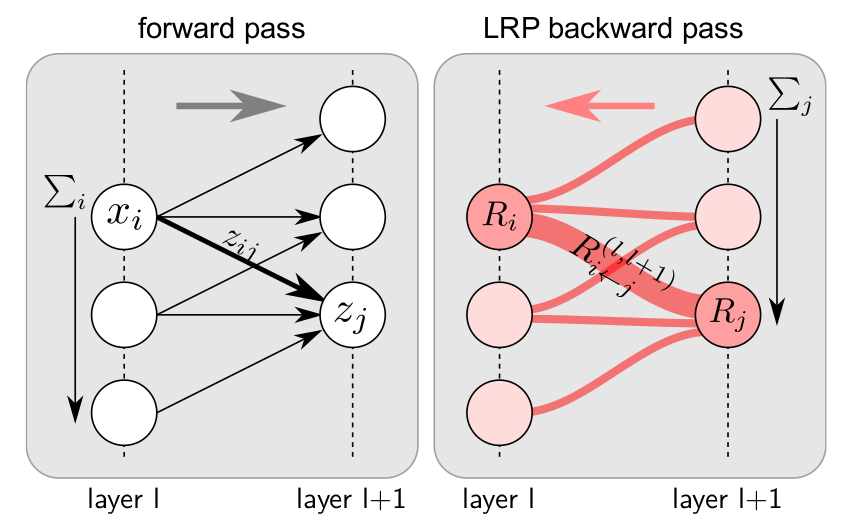
\includegraphics[width=0.3\textheight]{LRP_scheme.png}
		\caption[LRP-Schema]{Forward- und \ac{lrp}-Backward-pass}
		\source{\cite{lapuschkin}}
		\label{im:lrp_schema}
	\end{figure}
	
	 \noindent Bei der \textbf{Gamma-Regel (LRP-$\gamma$)} werden positive Gewichte zwischen den Netzschichten höher bewertet. Zusätzlich zum Positivteil in $z_{ij}$ wird ein mit $\gamma$ gewichtetes Vielfaches des Positivteils addiert. Es ergibt sich:
	
	\begin{equation}
		R_{i\leftarrow j}^{(l,l+1)} = \sum_j{\frac{x_j \cdot (w_{ij}+ \gamma w_{ij}^+)}{\sum_j{x_i \cdot (w_{ij} + \gamma w_{ij}^+)}}R_j^{(l+1)}}.
	\end{equation}
	
	\noindent Durch die Wahl von $\gamma$ lassen sich hier die positiven Anteile steuern. Für größere Werte $\gamma$ verschwinden die negativen Anteile. Mit dieser Formulierung bleiben die positiven und negativen Anteile der Relevanz beschränkt und es ergeben sich robustere Ergebnisse. Dieser asymmetrisch gewichtete Ansatz ist verwandt mit der \ac{lrp}-$\alpha/\beta$-Regel. Für $\gamma \to \infty$ erhalten wir die \ac{lrp}-$\alpha/\beta$-Regel mit $\alpha=1,\beta=0$.
	
	
	\begin{figure}[ht]
		\centering
		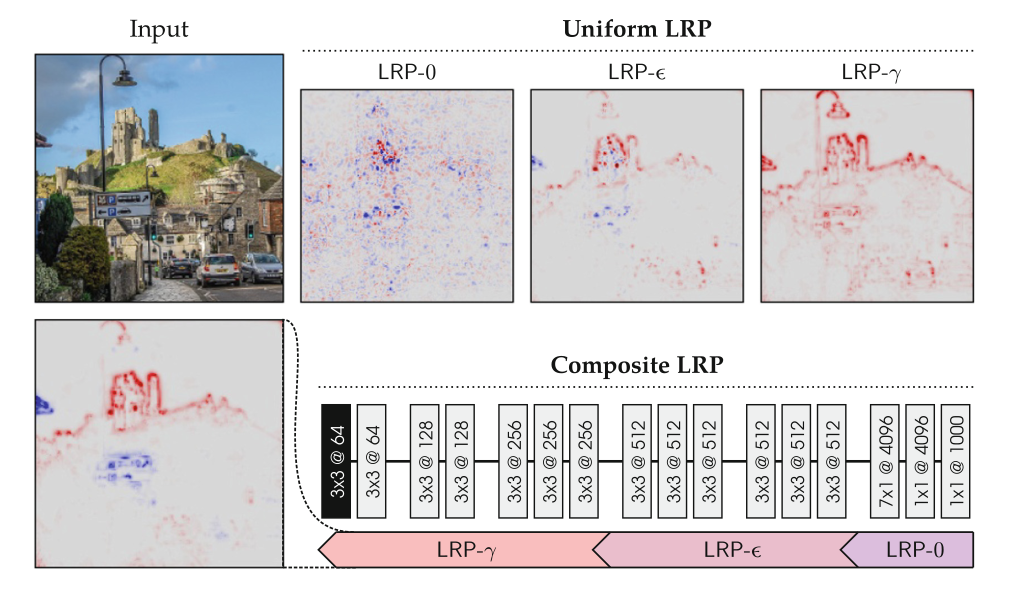
\includegraphics[width=0.3\textheight]{composite_lrp.png}
		\caption[Composite-LRP]{Composite-\ac{lrp}, $\varepsilon=0.25std, \gamma=0.25$, wobei std für die Standardabweichung des Datensatzes steht.}
		\source{\cite{samek2019explainable}}
		\label{im:composite_lrp}
	\end{figure}
	
	\begin{comment}
	Hier\footnote{https://towardsdatascience.com/indepth-layer-wise-relevance-propagation-340f95deb1ea} werden einige Bereiche vorgestellt, in denen LRP angewendet wurde.
	
	
	
	The overall idea of pixel-wise decomposition is to understand the contribution of a single pixel
	of an image x to the prediction f(x) made by a classifier f in an image classification task. We
	would like to find out, separately for each image x, which pixels contribute to what extent to a
	positive or negative classification result. Furthermore we want to express this extent quantita-
	tively by a measure. We assume that the classifier has real-valued outputs which are thre-
	sholded at zero. In such a setup it is a mapping f : R V ! R 1 such that f(x) > 0 denotes presence
	of the learned structure. Probabilistic outputs can be treated without loss of generality by sub-
	tracting 0.5. We are interested to find out the contribution of each input pixel x (d) of an input
	image x to a particular prediction f(x). The important constraint specific to classification con-
	sists in finding the differential contribution relative to the state of maximal uncertainty with
	respect to classification which is then represented by the set of root points f(x 0 ) = 0. One possi-
	ble way is to decompose the prediction f(x) as a sum of terms of the separate input dimensions
	
	x d respectively pixels:
	f 
	V
	X
	R d
	ð1Þ
	d1⁄41
	The qualitative interpretation is that R d < 0 contributes evidence against the presence of a
	structure which is to be classified while R d > 0 contributes evidence for its presence. In terms
	of subsequent visualization, which however will not be the scope of this paper, the resulting rel-
	evances R d for each input pixel x (d) can be mapped to a color space and visualized in that way
	as a conventional heatmap. One basic constraint will be in the following work that the signs of
	R d should follow above qualitative interpretation, i.e. positive values should denote positive
	contributi
	
	feedforward-Netzwerke
	Feedforward neural networks constitute a popular architec-ture type, ranging from simple multi-layer perceptrons andshallower convolutional architectures such as the LeNet-5[21]to deeper and more complex Inception [22] and VGG-likearchitectures [23]. These types of neural network commonlyuse ReLU non-linearities and first pass information throughastack of convolution and pooling layers, followed by severalfully connected layers. The good performance of feedforwardarchitectures in numerous problem domains, and the avail-ability as pre-trained models makes them a valuable standardarchitecture in neural network design.
	content...
	\end{comment}
	
	\noindent In Algorithmus \autoref{alg:lrp} ist die \ac{lrp} nochmals dargestellt, wobei die verwendete \textbf{LRP-0}-Regel durch die anderen vorgestellten Regeln ersetzt werden kann.
	
	\begin{algorithm}
		\hspace*{\algorithmicindent} \textbf{Input: } $R^{(L)} = f(x)$, model parameters \newline
		\hspace*{\algorithmicindent} \textbf{Output: } $\forall i,l: R_i^{(l)}$. 
		
		\caption{Layer-wise Relevance Propagation}
		\label{alg:lrp}
		
		\begin{algorithmic}
			\FOR{$l\in \lbrace L-1, ..., 1 \rbrace $}
				\STATE{$\forall i,j: R_{i\leftarrow j }^{(l,l+1)} = \frac{z_{ij}}{z_j}\cdot R_j^{(l+1)}$}
				\STATE{$\forall i: R_i^{(l)} \hphantom{=}= \sum_j{R_{i \leftarrow j}^{l,l+1}}$}			
			\ENDFOR
		\end{algorithmic}
	\end{algorithm}	

	

	
	
	
	\subsubsection{LRP für Tiefe Neuronale Netze} \label{lrp_für_dnn}
	In diesem Abschnitt gehen wir darauf ein, wie wir die oben vorgestellten \ac{lrp}-Regeln auf ein Tiefes \ac{nn} und damit auf die einzelnen unterschiedlichen Schichten dieses Netzes anwenden können \cite{LRP_DNN, lapuschkin, lrp_overview}.\\
	
	\noindent Wir bezeichnen mit $\sum_i$ die Summation über alle Neuronen einer bestimmten Schicht und mit $\sum_j$ die Summation über die Neuronen einer anderen Schicht. 
	
	\noindent Um innerhalb eines \ac{nn} Information von einer auf die darauffolgende Schicht abzubilden, werden häufig lineare Projektionen
	
	\begin{align}
		z_{ij} &= x_iw_{ij}\\
		x_j &= \sum_i{z_{ij} + b_j} \label{eq:linear_projection}
	\end{align}
	 oder komponentenweise Aktivierungsfunktionen
	 \begin{equation}
	 	x_j = \sigma(x_i)
	 \end{equation}
	 verwendet.
	 Der erste Fall beschreibt die häufig verwendeten vollständig verknüpften Netzschichten, während der zweite Fall die Verwendung nicht-li\-ne\-a\-rer Aktivierungsfunktionen oder Normalisierungsoperationen darstellt.
	 
	 \noindent Tiefe \acp{nn} führen nun eine Vielzahl solcher Schichten hintereinander aus.
	 
	 \noindent Eine häufig verwendete Aktivierungsfunktion ist die sogenannte ReLU-\-Ak\-ti\-vie\-rungs\-funk\-tion  $\sigma(x) = \max{\lbrace 0,x \rbrace}$, wobei die Abkürzung ReLU für rectified linear unit steht.
	 Diese wird in einer Vielzahl von Netzarchitekturen verwendet.
	 
	 \noindent Im Folgenden beschreiben wir, wie die \ac{lrp}-Regel \eqref{eq:lrp_regel} für die einzelnen Schichten, die in einem Inception-Netz auftreten, umgesetzt werden kann. Für die im Folgenden vorgestellten linearen, Pooling-, Aktivierungs-, Merge- und Normalisierungsschichten folgen wir der Ausführung in \cite{lapuschkin}.\\
	 
	 \noindent\textbf{Lineare Schichten:}\\
	 Netzschichten, die lineare Transformationen über einen Gewichtskernel implementieren, d.h. vollständig verknüpfte Schichten und alle Varianten von Convolutional-Schichten, implementieren die Funktion in \eqref{eq:linear_projection}.\\
	 
	 \noindent Seien mit $i$ die Eingabe- und mit $j$ die Ausgabe-Neuronen bezeichnet. Sei eine Relevanz $R_j^{(l+1)}$ gegeben. Eine Relevanz-Zerlegung erhalten wir nun durch die Wahl von $z_{ij}=x_iw_{ij}$ wie in \eqref{eq:linear_projection} und $z_j = x_i$, d.h. die Aktivierungen der Schicht $l+1$. Damit erhalten wir die rückwärts-gerichtete Relevanz-Nachricht 
	 \begin{equation}
	 	R_{i\leftarrow j}^{(l,l+1)} = \frac{x_iw_{ij}}{\sum_i{x_iw_{ij}+b_j}}\cdot R_j^{(l+1)} = \frac{z_{ij}}{z_j}\cdot R_j^{(l+1)},
	 \end{equation}
	wobei der Bias $b$ als konstant aktivierendes Neuron, das über die Gewichte $b_j$ mit den Ausgabe-Aktivierungen $x_j$ verbunden ist, interpretiert wird.
	Durch diese Interpretation des Bias als eigenes Neuron, geht in jedem Rückwärtsschritt Relevanz verloren. Eine Möglichkeit, dies zu beheben, wird in \cite{lapuschkin}[Kapitel 2.2.4] diskutiert.\\
	
	
	
	\noindent\textbf{Pooling-Schichten}\\
	Zu den Pooling-Schichten gehören das Sum-, Average- und Max-Pooling. Für alle drei lässt sich auch hier eine entsprechende \ac{lrp}-Regel direkt anwenden.
	Sowohl das Sum- als auch das Average-Pooling lassen sich als Convolutional-Schicht verallgemeinern. Dafür wird $w_{ij}=1$ für das Sum-Pooling und ${w_{ij}=1/n}$ für das Average-Pooling gewählt.
	
	\noindent In unserer Version des Inception-Netzes verwenden wir das Max-Pooling. Dieses implementiert die Funktion
	\begin{equation}
		x_j = \max_i{(x_i)}
	\end{equation}
	für jedes Ausgabe-Neuron $j$ über alle Eingabe-Neuronen $i$. Die Relevanz muss nun an das maximal aktivierende Eingabe-Neuron übertragen werden, d.h.:
	\begin{equation}
	R_{i \leftarrow j}^{(l,l+1)} = \begin{cases}
	R_j^{(l+1)} & \text{falls  } i =\argmax_i{(x_i)}\\
	0			& \text{sonst.}
	\end{cases}
	\end{equation}
	Die Vorschrift für den Fall, dass mehrere Neuronen dasselbe Maximum annehmen, lässt sich leicht einschließen.\\
	
	
	\noindent\textbf{Aktivierungsschichten}\\
	Für die komponentenweise angewandten Aktivierungsfunktionen werden keine Eingabe-Aktivierungen untereinander kombiniert. Es ergibt sich für die Relevanz-Nachricht
	
	\begin{equation}
		R_{i\leftarrow j}^{(l,l+1)} = \begin{cases}
		R_j^{(l+1)} & \text{falls  } i=j\\
		0 &\text{sonst,}
		\end{cases}
	\end{equation} d.h. die eingehende Relevanz wird unverändert als Ausgabe weitergegeben.\\
	
	
	
	\noindent\textbf{Merge-Schichten}\\
	\noindent In \autoref{chapter:inception} hatten wir den Aufbau von Inception-Netzen und auch den verwendeten Inception-Modulen besprochen. Hierbei treten sogenannte Merge-Schichten auf, bei denen Information von verschiedenen Netzschichten zusammengeführt werden.
	
	\noindent In \cite{lapuschkin} wird dabei zwischen \textit{Merge by aggregation} und \textit{Merge by concatenation} unterschieden. Dabei beschreibt ersteres die Zusammenführung verschiedener Netz-Aktivierungen durch Addition oder Subtraktion. Diese Netzschicht implementiert die Funktion
	\begin{equation}
		x_j = x_{1,j} + x_{2,j} + ... + x_{n,j},
	\end{equation}
	wobei die Eingabe-Tensoren $x_1, ..., x_n$ dieselbe Dimension besitzen und kom\-po\-nen\-ten\-wei\-se am Index $j$ zusammengeführt werden sollten. Analog zu den komponentenweisen Aktivierungsfunktionen tritt hier keine Vermischung an Information auf und die Relevanz-Zerlegung kann analog zum linearen Fall mit 
	\begin{align}
		z_{ij} &= x_{ij}\\
		x_j &= \sum_i{z_{ij}}
	\end{align} umgesetzt werden. Folglich kann \eqref{eq:lrp_regel} ohne Abänderung und mit der Wahl $x_j= z_j$ verwendet werden. Der für uns ebenfalls interessante zweite Fall beschreibt die Konkatenierung am Ende eines Inception-Moduls. Auch hier entsteht aufgrund der Konkatenierung entlang einer Tensor-Achse keine Interaktion zwischen den einzelnen Netzschichten. Zum forward-pass
	\begin{equation}
		x_j = [x_{1,j}, x_{2,j}, ... , x_{n,j}],
	\end{equation}
	wobei $j$ die Tensor-Achse orthogonal zur Konkatenierungs-Achse bezeichnet, ergibt sich die einfache Relevanz-Zerlegung
	
	\begin{equation}
		[R_{1,j}^{(l)}, R_{2,j}^{(l)}, ..., R_{n,j}^{(l)}] = R_j^{(l+1)}.
	\end{equation}\\
	
	\noindent\textbf{Normalisierungsschichten}\\
	Häufig werden Netzschichten benutzt, die eine Normalisierung während des Trainings durchführen. Bei der sogenannten Batch-Normalisierung wird eine Normalisierung über dem Mini-Batch an ausgewählten Trainingsdaten durchgeführt. Durch die Verwendung der Batch-Normalisierung wird die Konvergenz und damit die Trainingszeit des \ac{nn} verbessert.\\
	
	\noindent Die Batch-Normalisierung führt eine komponentenweise definierte Funktion 
	\begin{equation}
		z = \frac{x -\mu_\mathcal{B}}{\sqrt{\sigma_\mathcal{B}^2 + \epsilon}}\gamma + \beta
	\end{equation}
	aus. Dabei sind $\gamma$ und $\beta$ zwei Parameter, die die Datenpunkte skalieren und verschieben und während des Trainings gelernt werden. $\mu_\mathcal{B}$ und $\sigma_\mathcal{B}^2$ sind Mittelwert und Varianz des aktuellen Mini-Batches. Nach dem abgeschlossenen Training werden $\mu_\mathcal{B}$ und $\sigma_\mathcal{B}^2$, fixiert, indem sie über den gesamten Datensatz berechnet werden. Die Skalierungsoperation können wir schreiben als $s=\gamma \cdot (\sigma_\mathcal{B}^2 + \epsilon)^{\frac{1}{2}}$. Für die Batch-Normalisierung während der Inferenz ergibt sich dann die Abfolge von (komponentenweisen) Additionen und Multiplikationen:
	\begin{align}
		x' &= x- \mu_\mathcal{B}, \label{eq:translation1}\\
		x'' &= x' \cdot s,\\
		z &= x'' + \beta. \label{eq:translation2}
	\end{align}
	Durch die Betrachtung der Translationen (\autoref{eq:translation1}, \autoref{eq:translation2}) als additive Merge-Operationen lässt sich die Relevanz-Übertragung analog zum Merge- und Aktivierungs-Abschnitt formulieren als:
	
	\begin{equation}
		R^{(l)} = \frac{x \odot s \odot R^{(l+1)}}{z},
	\end{equation}
	\noindent wobei $\odot$ die punkt-weise Multiplikation beschreibt.\\
	
	\noindent Damit haben wir \ac{lrp}-Regeln für alle Netzschichten im Inception-Netz besprochen, sodass wir durch die wiederholte Ausführung der \ac{lrp}-Regeln zu einer Netzeingabe eine Heatmap erhalten.\\
	
	%\noindent Eine Beispielausgabe der \ac{lrp} für ein Inception-Netzwerk und ein korrumpiertes Verkehrsschild findet sich in \autoref{vergleich_original_lrp}
	
	
	
	
	 









	\chapter{Untersuchungen und Ergebnisse} \label{chapter_results}
	
	In diesem Kapitel stellen wir vor, welche Untersuchungen im Rahmen dieser Masterarbeit durchgeführt wurden und welche Ergebnisse wir erhalten haben.
		
	\section{Setting und Methoden}
	In diesem Abschnitt stellen wir das verwendete \ac{nn}, den Datensatz und den Trainingsprozess vor.
	
	\subsection{Verwendetes Netz}
	Wir verwenden eine vereinfachte Version eines Inception v3-Netzes, das aus drei größeren Teilen besteht. Den ersten Teil bildet ein Inception-Modul (vgl. \autoref{chapter:inception}). Der zweite Teil besteht aus vier Blöcken, bei denen jeder Block aus einer Pooling- und einer Batch-Normalisierungsschicht sowie einer Convolutional Layer aufgebaut ist. Abgeschlossen wird das \ac{nn} mit drei linearen Schichten, die jeweils eine ReLu-Aktivierungsfunktion besitzen und durch Dropout-Schichten getrennt sind. Der Programmcode ist in python geschrieben. Als Bibliothek für \acp{nn} verwenden wir pytorch.
	  
	\noindent Im Unterschied zu den offiziellen Inception-Netzen besitzt dieses \ac{nn} keinen \textit{stem} aus Convolutional Layern, d.h. eine bestimmte Anzahl an Convolutional Layern, die dem ersten Inception-Modul vorangestellt sind, sondern beginnt direkt mit diesem.\\
		
	\noindent Mit etwa einer Million trainierbaren Parametern ist das \ac{nn} im Vergleich zum offiziellen Inception v3-Netz mit über 24 Millionen Parametern deutlich kleiner, wodurch der Trainingsprozess beschleunigt ist.\\
	\noindent Für ein Training des \ac{nn} auf nicht manipulierten Daten (\autoref{chapter:dataset}) erhalten wir eine Testgenauigkeit von 97.8 Prozent. Der Aufbau des \ac{nn} ist in \autoref{im:inceptionv3layout} dargestellt.
	
	
	\begin{figure}
		\centering
		
		\centering
		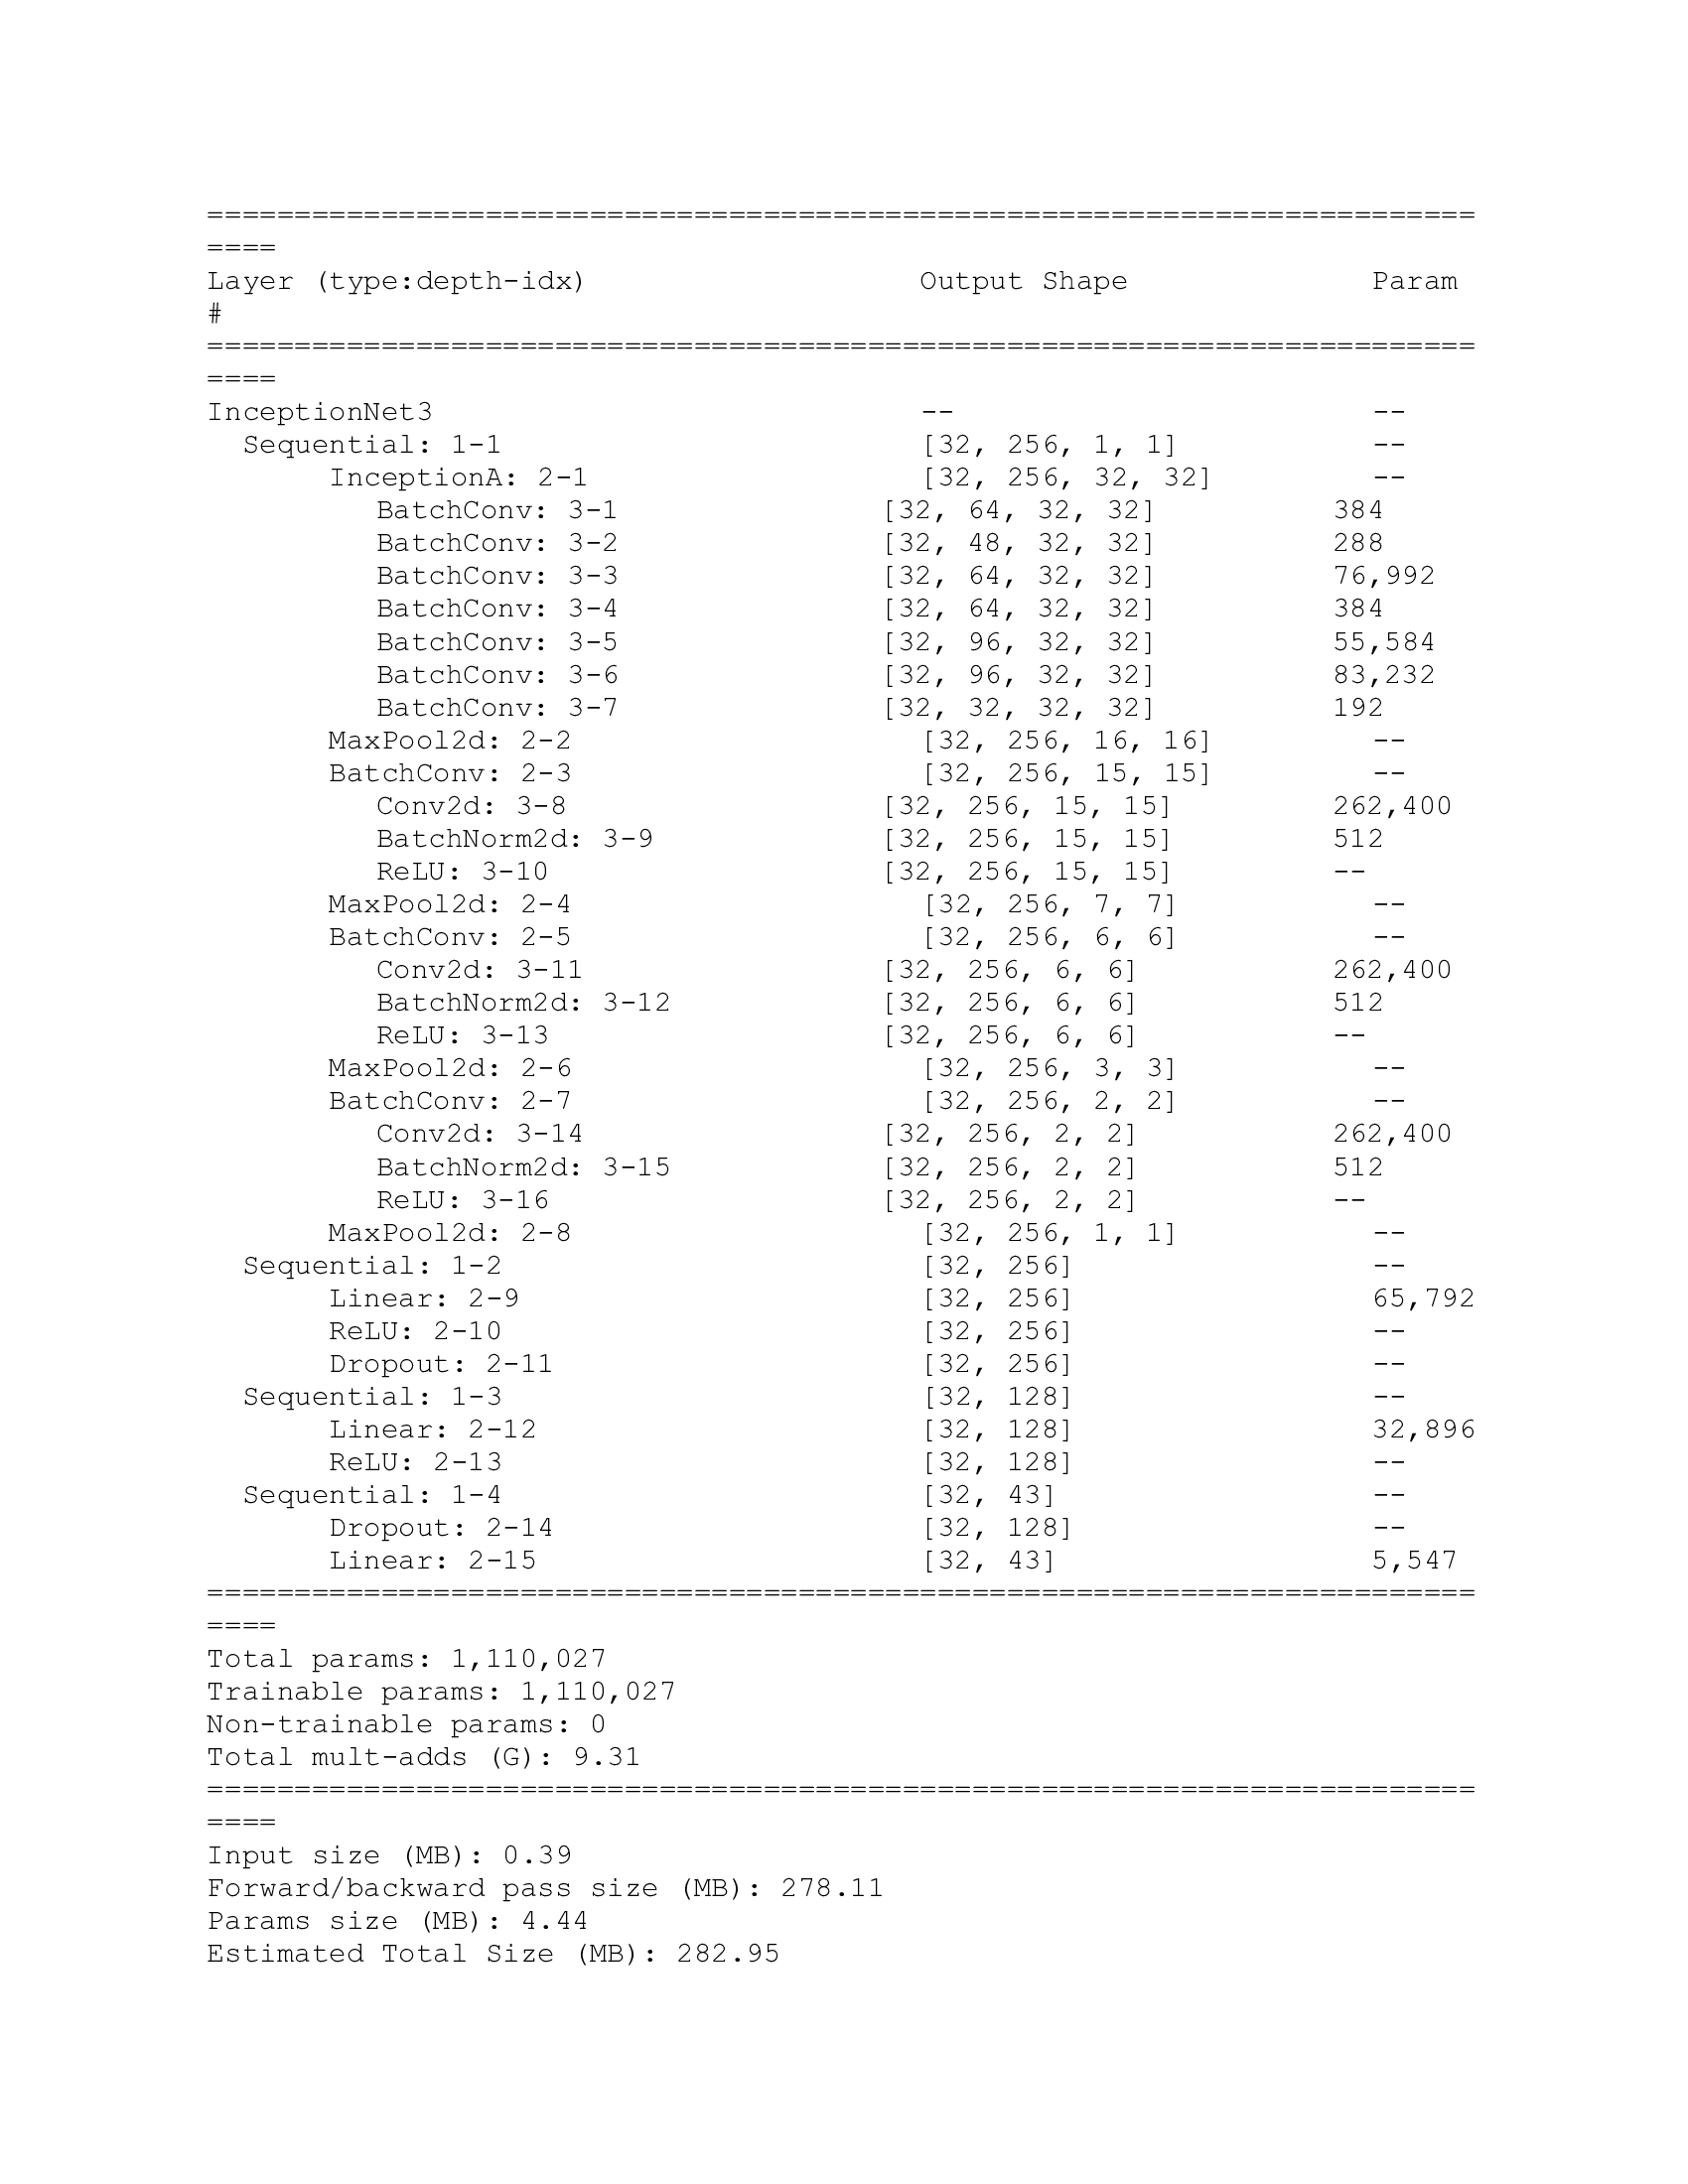
\includegraphics[width=\linewidth]{inceptionNet_layout.jpg}
		
		\caption{Aufbau des verwendeten Inception-Netzes.}
		
		
		\label{im:inceptionv3layout}
	\end{figure}
	
	
	\subsection{Datensatz} \label{chapter:dataset}
	Als Datensatz verwenden wir den Datensatz German Traffic Sign Recognition Benchmark \cite{GTSRB_dataset}. Dieser besteht	aus 52.001 Bildern von Verkehrsschildern aus 43 verschiedenen Klassen der Pixelgröße $32 \times 32$. Etwa 75 Prozent der Bilder wird für das Training, die anderen 25 Prozent für das Testen benutzt. Der Datensatz wurde ursprünglich in	einem Wettbewerb auf der International Joint Conference on Neural Networks (IJCNN) im Jahr 2011 vorgestellt. In einer Klasse befinden sich jeweils mehrere Bilder desselben realen Verkehrsschildes zu unterschiedlichen Zeitpunkten, da die Bilder aus einer Videosequenz herausgeschnitten sind.  Aufnahmen desselben Verkehrsschildes kommen nicht übergreifend in Training-, Validierung- oder Testdatensatz vor. Ein Beispielbild jeder einzelnen Klasse im Datensatz ist in \autoref{im:dataset} gegeben.
	
	\begin{figure}[ht]
		\centering
		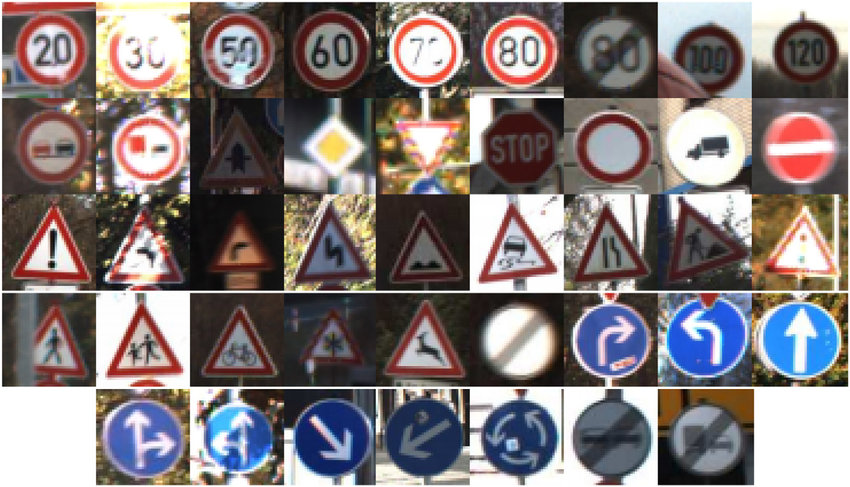
\includegraphics[width=0.6\textheight]{gtsrb_overview.png}
		
		\caption{Beispielbilder der 43 verschiedenen Klassen im Datensatz (GTSRB)}
		\source{\cite{GTSRB_dataset}}
		\label{im:dataset}
		%\source{https://www.mathworks.com/help/deeplearning/ref/no\_padding\_no\_strides.gif}
	\end{figure}
	
	
	
	\subsection{Training}
	Für das Training des Netzes benutzen wir die Cross-Entropy-Verlustfunktion. Für das Einlesen der Daten benutzen wir, sofern nicht anders angegeben, die in \autoref{augmentation} gezeigten Augmentierungen.
	
	\begin{lstlisting}[language=Python, caption=Augmentierung beim Einlesen der Daten, label=augmentation]
	__train_transform = transforms.Compose(
	[
	transforms.RandomResizedCrop((image_size, image_size), 
	scale=(0.6, 1.0)),
	transforms.RandomRotation(degrees=15),
	transforms.ColorJitter(brightness=0.1, contrast=0.1, 
	saturation=0.1, hue=0.1),
	transforms.RandomAffine(15),
	transforms.RandomGrayscale(),
	transforms.Normalize(	mean=[0.485, 0.456, 0.406], 
	std=[0.229, 0.224, 0.225]),
	transforms.ToTensor()
	]
	\end{lstlisting}
	Dabei wählt \textit{RandomResizedCrop} einen abhängig von der Eingabegröße des Bildes festgelegten Bildausschnitt und skaliert diesen wieder auf eine feste Bildgröße. \textit{RandomRotation} rotiert das Bild um einen zufälligen Winkel zwischen -15 und 15 Grad. \textit{ColorJitter} ändert zufällig
	die Helligkeit, den Kontrast sowie die Sättigung. \textit{RandomAffine} führt eine affine Transformation mit maximal 15 Grad Rotation durch. \textit{RandomGrayscale}
	erstellt aus der Eingabe mit einer Wahrscheinlichkeit von $p = 0.1$ ein Graustufenbild. \textit{Normalize} normalisiert das Bild für einen gegebenen Mittelwert $mean$ und die Varianz $std$. \textit{ToTensor} konvertiert das Bild in einen \textit{torch.FloatTensor} der Form $(C
	\times H \times W)$ im Intervall $[0.0, 1.0]$.
	
	\noindent Die Werte von mean und std variieren für alle ausgeführten Poisoning-Angriffe. Anstatt beide für jeden Angriff erneut zu berechnen, verwenden wir die von pytorch empfohlenen Werte für vortrainierte \acp{nn}, die auf dem Datensatz ImageNet\cite{imagenet} basieren.\\
	\noindent Wir trainieren das \ac{nn} über maximal 100 Epochen und benutzen \textit{early stopping} mit $patience=20$, d.h. wir brechen das Training ab, falls sich der Fehler auf dem Validierungsdatensatz in den letzten 20 Epochen nicht verringert hat. Die verwendete Implementierung ist eine modifizierte Version von Bjarte Mehus Sunde \cite{early-stopping-pytorch}, die wiederum auf PyTorch Ignite \cite{pytorch-ignite} basiert.\\
	
	%\section{Einlesen der Daten bei AC}
	%Ohne Transformationen, wie den Testdatensatz.
	\subsection{Ausgeführte Poisoning-Angriffe}
	In den folgenden Abschnitten werden wir erklären, wie wir die beiden Angriffe jeweils umgesetzt, d.h. wie wir den Datensatz manipuliert haben, um erfolgreich eine Hintertür im \ac{nn} zu implementieren.
	
	\subsubsection{Standard-Poisoning-Angriffe}
	Um eine Hintertür im gewählten \ac{nn} zu implementieren, benötigen wir eine Start- und Zielklasse, einen Auslöser und einen Anteil an zu korrumpierenden Bildern. \\
	
	\noindent In \autoref{hallo} sind einige Klassen der Verkehrsschilder und deren Anzahl im Datensatz aufgelistet, die für einen \ac{pa} interessant sein könnten. Die Anzahl der ’Halt! Vorfahrt gewähren’-Schilder im Trainingsdatensatz beträgt etwa 690 Aufnahmen. Diese wurden von insgesamt nur 24 verschiedenen ’Halt! Vorfahrt gewähren’-Schildern aufgenommen.
	Für die Wahl der Start- und Zielklasse wäre vermutlich aus Sicht des Angreifers maximaler Schaden erreicht, falls ein Stopp-Schild, versehen mit einem Auslöser, als Geschwindigkeitsbegrenzung von 120 km/h klassifiziert würde.
	
	\noindent Da wir bei dieser Art von \ac{pa} zusätzlich das entsprechende Label abändern, d.h. die korrumpierten Bilder in die Zielklasse verschieben, wählen wir für den Angriff nicht die Stopp-Schild-Klasse, da die Anzahl an Schildern in dieser Klasse vergleichsweise gering ist.\\
	
	\noindent Stattdessen wählen wir als Startklasse die 50 km/h-Schilder, da diese von den für einen Angriff interessanten Schildern den höchsten Anteil im Datensatz darstellen.\\

	\begin{table}[h]\caption[Verteilung bestimmter Verkehrsschilder im Datensatz]{Für einen \ac{pa} interessante Klassen und die zugehörige Anzahl an Bildern.}
		\label{hallo}
		\begin{tabular}[h]{c|c}
			Verkehrsschilder & Anzahl an Bildern \\ \hline
			’Zulässige Höchstgeschwindigkeit: 20km/h’& 180 \\
			’Zulässige Höchstgeschwindigkeit: 30km/h’ & 1980 \\
			’Zulässige Höchstgeschwindigkeit: 50km/h’	& 2010 \\
			’Zulässige Höchstgeschwindigkeit: 60km/h’	& 1260 \\
			’Zulässige Höchstgeschwindigkeit: 70km/h’	& 1770 \\
			’Zulässige Höchstgeschwindigkeit: 80km/h’	&1650 \\
			’Halt! Vorfahrt gewähren’					&	690
		\end{tabular}
		
		
	\end{table}
	
	\noindent Als Zielklasse wählen wir die Schilder mit zulässiger Höchstgeschwindigkeit 80 km/h.
	Als Auslöser verwenden wir einen quadratischen Pixelblock, der einen gelb-grünen Sticker auf dem entsprechenden Verkehrsschild darstellen soll. Dazu ändern wir die Werte des Pixelblocks auf den hexadezimalen Farbcode $\#f5ff00$ ab. Für die Seitenlänge des Auslösers wählen wir $s=1,2,3$~Pixel. \\
	\noindent Da wir keine Bounding-Box zur Verfügung haben, mit der wir den Sticker auf einem Schild an
	derselben Stelle platzieren können, fügen wir den Sticker zufällig so ein, dass die
	linke obere Ecke innerhalb eines festen Fensters $([x_{min}, x_{max}], [y_{min}, y_{max}])$ gesetzt
	wird, wobei dies die Pixel-Koordinaten in der Breite bzw. Höhe des Bildes sind.
	Die Pixel sind in der üblichen Lesereihenfolge durchnummeriert. Ein korrumpiertes
	Bild ist in \autoref{im:SPA} dargestellt. \\
	
	
	
	\begin{figure}[ht]
		\centering
		
\includegraphics[width=0.15\textheight]{1450_poison.jpeg}
		
		
		\caption[Visualisierung des Standard-Angriffs]{Korrumpierter Datenpunkt aus  '50 km/h' mit gelb-grünem Sticker und dem Label '80 km/h'.}
		
		\label{im:SPA_implementation}
	\end{figure}
	
	
	\subsubsection{Label-konsistente Poisoning-Angriffe}
	
	Für die Störung des Bildes bei \acp{lkpa} nutzen wir ein projektives Gradienten-Verfahren mit  $n=5$ Iterationen und einer Schrittweite $step\_size = 0.015$. Um den Auslöser nicht durch die Augmentierung beim Einlesen der Trainingsdaten (vgl. \autoref{augmentation}) abzuschneiden, verschieben wir diesen soweit in Richtung der Bildmitte, dass der $3\times 3$ große Sticker jeweils einen Abstand von 10 Pixeln zum unteren und rechten Rand besitzt.
	Anschließend wird das \ac{nn} wieder mit dem manipulierten Datensatz trainiert.
	
	
	\subsection{Detektionsverfahren}
	In diesem Abschnitt beschreiben wir, wie wir die verschiedenen Clustering-Algorithmen zur Detektion von \ac{pa} angewendet haben und welche Vorverarbeitung der jeweiligen Daten durchgeführt wurde.
	
	\subsubsection{Clustering auf den Rohdaten}
	
	Für das Clustering direkt auf den Bilddaten werden die Bilder als Graustufenbild eingelesen und anschließend eine Dimensionsreduktion durchgeführt. Dazu nutzen wir einerseits eine Hauptkomponentenanalyse \cite{pca} und andererseits eine Unabhängigkeitsanalyse. 
	
	\noindent Wir reduzieren die Bilder auf 10 Dimensionen und führen das $k$Means-Clus\-ter\-ing anschließend bezüglich der $L^2$-Distanz durch. Die Implementierungen entnehmen wir der Machine-Learning-Toolbox sklearn \cite{sklearn}. Dabei werden für einen Durchlauf des Clusterings maximal 300 Iterationen verwendet. Initialisiert wird mit der $k$Means$++$ -Initialisierung (vgl. Algorithmus \autoref{alg:kmeans++_init}). Zusätzlich werden insgesamt 10 Durchläufe wiederholt und als finales Ergebnis wird das Clus\-ter\-ing mit dem kleinsten Gesamtfehler akzeptiert.	
	
	\subsubsection{Activation-Clustering}
	Beim \ac{ac} nutzen wir analog zu \cite{AC} die Aktivierungen der vorletzten Netzschicht. Diese reduzieren wir ebenfalls mit einer Hauptkomponentenanalyse auf 10 Dimensionen. Für das Clustering selbst verfahren wir analog zum Clustering auf den Rohdaten.
	
	\subsubsection{Heatmap-Clustering}
	Für das Heatmap-Clustering müssen zunächst die Heatmaps berechnet, weiterverarbeitet und anschließend das $k$Means-Clustering durchgeführt werden. Wir erklären die einzelnen Schritte im Folgenden.\\
	
	\noindent\textbf{Berechnung der Heatmaps}\\
	Wir nutzen die \ac{lrp}-$\varepsilon$-Regel (vgl. \autoref{chapter_lrp}), um Heatmaps der verdächtigen Klasse (50 km/h) bezüglich der Entscheidung für die Klasse (80~km/h) zu berechnen. Wir hatten uns für diese Regel nach einem Vergleich mit der $\beta$-Regel entschieden, die nicht zu besseren Heatmaps oder Cluster-Ergebnissen geführt hatte.
	
	\noindent Es existieren mehrere \ac{lrp}-Implementierungen sowohl für pytorch als auch TensorFlow. Da wir mit \acp{nn} in pytorch arbeiten, haben wir uns für die Version von Böhle \cite{moboehle} entschieden. Diese entstand im Rahmen der Forschungsarbeit \cite{lrp_alzheimer}, in der eine Alzheimer-Diagnose aufgrund von Bilddaten vorgenommen wird. Dabei werden sogenannte \textit{pytorch hooks} verwendet, um auf einzelne Netzschichten zuzugreifen. Der Programmcode überzeugt dadurch, dass einzelne Arten von Netzschichten leicht ergänzt werden können. Eine modifizierte Version ermöglicht es uns, die Implementierung auch für das Inception-Netz zu benutzen. Dabei haben  wir die \ac{lrp}-Regeln für die Inception-Module sowie die Batch-Normalisierungsschichten implementiert (vgl. \autoref{lrp_für_dnn}).
	
	\noindent Weitere Implementierungen sind beispielsweise das \ac{lrp}-Tutorial in pytorch für VGG16 \cite{lrpmontavon}, TorchLRP \cite{torchlrp} oder Zennit\cite{zennit}.\\
	
	\noindent\textbf{Verarbeitung der Heatmaps}\\
	Die \ac{lrp}-Ausgabe zu einer Bildeingabe besitzt die Größe $[32 \times 32 \times 3]$, wobei 3 für die einzelnen Farbkanäle steht. Es sind sowohl positive als auch negative Relevanz-Werte möglich. Dabei deutet ein positiver Wert darauf hin, dass dieser Bereich entscheidend für die Einordnung in diese Klasse ist. Wir addieren die Relevanzen auf allen 3 Farbkanälen und normalisieren das Ergebnis anschließend auf das Intervall $[0,1]$. Die so modifizierte \ac{lrp}-Ausgabe zu einem originalen korrumpierten Bild ist in \autoref{vergleich_original_lrp} abgebildet. \\
	
	\begin{figure}
		\centering
		\begin{subfigure}{.5\textwidth}
			\centering
			
\includegraphics[width=.4\linewidth]{1450_poison}
			%\caption{Verkehrsschild der Klasse 'Höchstgeschwindigkeit: 50km/h' versehen mit einem 3x3 Sticker und dem Label 'Höchstgeschwindigkeit: 80km/h'}
			
		\end{subfigure}%
		\begin{subfigure}{.5\textwidth}
			\centering
			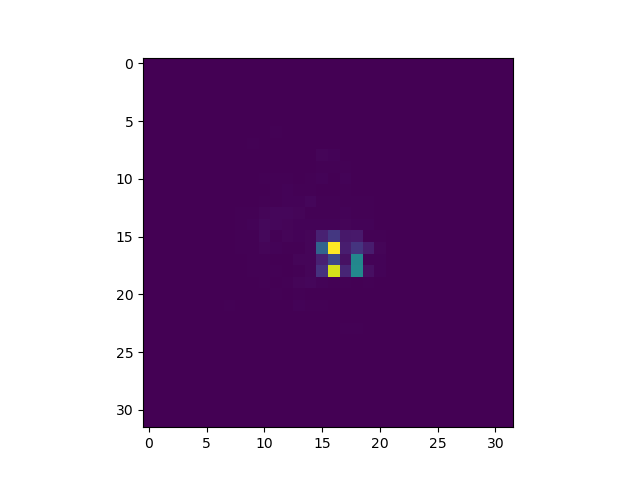
\includegraphics[width=.7\linewidth]{1450_poison_lrp.png}
			%\caption{Zugehörige Heatmap bezüglich der Klasse 'Höchstgeschwindigkeit: 80km/h'}
			
		\end{subfigure}
		\caption[(Optischer) Vergleich von korrumpiertem Datenpunkt und berechneter Heatmap.]{(Optischer) Vergleich von korrumpiertem Datenpunkt und berechneter Heatmap. \textbf{Links}: Verkehrsschild der Klasse 'Höchstgeschwindigkeit: 50 km/h' versehen mit einem $3\times 3$ Sticker und dem Label 'Höchstgeschwindigkeit: 80 km/h'. \textbf{Rechts}: Zugehörige Heatmap bezüglich der Klasse 'Höchstgeschwindigkeit: 80 km/h'.}
		%\source{\cite{AC}}
		
		\label{vergleich_original_lrp}
	\end{figure}
	
	
	
	
	\noindent Damit wir Maße auf zwei verschiedenen metrischen Räumen vergleichen können, wählen wir zunächst diejenigen Pixel aus, die die ersten 99 Prozent der Gesamtmasse beinhalten.\\
	
	\begin{figure}[h]
		
		\begin{center}
			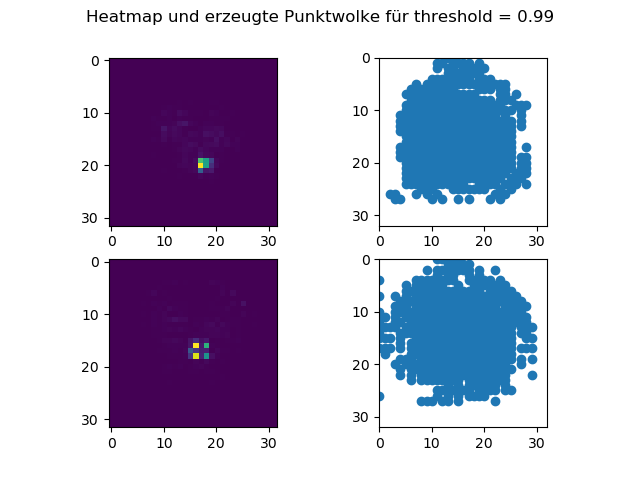
\includegraphics[width=0.5\textheight]{HeatmapPunktwolke99.png}
			
		\end{center}
		\caption{Auswahl der relevantesten Pixel (bis zu $99\%$ der Gesamtmasse) zweier Heatmaps bei korrumpierten Bildern.}
		\label{wölkchen}
	\end{figure}
	
	\noindent In \autoref{wölkchen} sind links zwei Heatmaps korrumpierter Bilder sowie rechts die Positionen der ausgewählten Pixel abgebildet. In der Auswahl auf der rechten Seite können wir sehen, dass eine kreisförmige Auswahl getroffen wird, die ungefähr den Verkehrsschildern entspricht.\\
	
	
	
	\noindent\textbf{Bestimmung der Gromov-Wasserstein-Distanzen}\\
	Für die wie oben beschrieben verarbeiteten Heatmaps benötigen wir für die \ac{gwd} eine Distanzmatrix auf der Heatmap sowie die Gewichte für jeden relevanten Pixelpunkt.
	
	\noindent Um für die Heatmaps, interpretiert als metrische Maßräume, verschiedene metrische Räume zu erhalten, wählen wir jeweils die Gewichte und Koordinaten der $n$ relevantesten Pixel, die zusammen 99 Prozent der Summe der Relevanzen der Heatmap darstellen. 
	
	\noindent Für die gewählten Koordinaten berechnen wir eine Distanzmatrix $C \in \mathbb{R}^{n \times n}$ bezüglich der $L^2$-Distanz unter Verwendung der SciPy-Toolbox \cite{scipy}.
	Die ausgewählten Relevanzen fassen wir als Vektor $p \in \mathbb{R}^n$ zusammen.\\
	
	\noindent Für die anschließende Berechnung der regularisierten \ac{gwd} und -Baryzentren verwenden wir die Python Optimal Transport Toolbox (POT) \cite{pot}. In \cite{cuturi2013sinkhorn} werden verschiedene Werte für den Regularisierungsparameter $\varepsilon$ (vgl. \autoref{gwd} angegeben. Diese sind $\varepsilon = 0.02, 0.1, 1.0$ Im zugehörigen Beispiel von POT \cite{pot_example} wird $\varepsilon = 0.0005$ verwendet. Als Regularisierungs-Parameter verwenden wir $\varepsilon=0.1$.\\	
	
	
	
	\noindent\textbf{$k$Means-Clustering}\\
	Für das Clustering verwenden wir die $k$Means$++$-Initialisierung und brechen das Clustering ab, falls sich dieses innerhalb eines Update-Schritts nicht mehr ändert oder eine maximale Iterationszahl von 20 Iterationen erreicht wird.
	
	
	
	\section{Ergebnisse} \label{chapter_comparisons}
	
	In diesem Kapitel fassen wir die Ergebnisse der Detektion von \acp{pa} mithilfe des modifizierten Clusterings auf den Heatmaps zusammen. Dabei gehen wir auf die unterschiedlichen Arten von \acp{pa} ein und vergleichen die Detektion jeweils mit dem \ac{ac}. Zu Beginn geben wir das Clusterings auf den Rohdaten als Referenzwert an.\\
	
	\noindent Die Qualität eines Angriffs, angegeben durch die \ac{aer}, ist abhängig von der Größe des Anteils an korrumpierten Daten innerhalb einer Klasse. \autoref{fig:aerspas3} zeigt, wie sich die \ac{aer} für verschiedene Werte zwischen 0.125~Prozent und 33 Prozent an korrumpierten Daten verhält. 

	\begin{figure}[h]
		\centering
		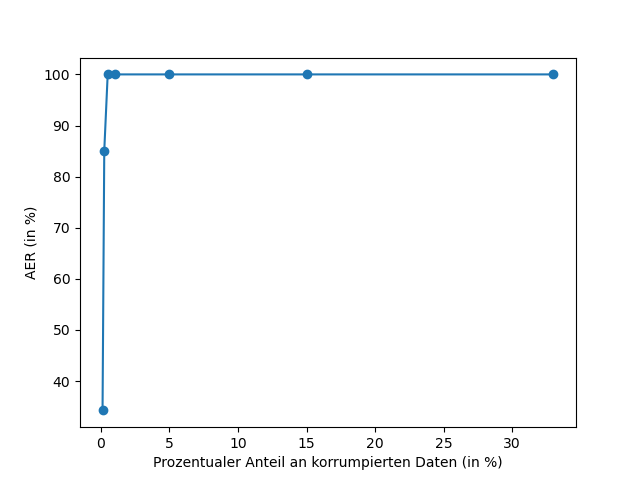
\includegraphics[width=0.5\linewidth]{AER_SPAs3.png}
		\caption{Angriffserfolgsrate für verschiedene prozentuale Anteile bei s=3.}
		\label{fig:aerspas3}
	\end{figure}
	
	%\noindent Es ist auffällig, dass die Angriffe bereits für alle Werte über 0.5 Prozent sehr gut funktionieren. Bei 0.25 Prozent korrumpierten Daten wird noch immer eine \ac{aer} von 85.07 Prozent erreicht.
	\noindent Bei der Durchführung von Standard-\ac{pa} zeigt sich, dass selbst für sehr kleine Anteile erfolgreiche Angriffe implementiert werden können. Beispielsweise konnten wir sogar bei einem Anteil von 0.5 Prozent (das entspricht nur 8 korrumpierten Bildern) noch eine \ac{ac} von 99.87 Prozent erreichen. Bei 2 korrumpierten Bildern lag die Erfolgsrate bei 35.6 Prozent. Für alle korrumpierten Anteile über 0.5 Prozent ergeben sich perfekte Angriffe mit einer \ac{aer} von 100 Prozent.
	
	\noindent Wir konnten beobachten, dass die Qualität des angegriffenen Netzes auf nicht korrumpierten Daten für alle durchgeführten Angriffe bei über 96 Prozent liegt. Deshalb werden wir diese Kennzahl als Qualität des Angriffs nicht jeweils zusätzlich angeben.\\
	
	\noindent Im Folgenden geben wir für jedes Verfahren jeweils die \ac{acc}, die \ac{tpr} sowie die \ac{tnr} (vgl. \autoref{chapter:detectionevaluation}) an. Dabei ist zu beachten, dass die \ac{tpr} im Vergleich zur \ac{tnr} die für uns deutlich wichtigere Kennzahl ist. Das gilt deshalb, weil es wichtiger ist, alle korrumpierten Datenpunkte im Datensatz zu entfernen, um alle Hintertüren nach einem erneuten Training auf dem bereinigten Datensatz zu eliminieren. 
	
	
	\subsection{Clustering auf den Rohdaten}
	Für das Clustering auf den Rohdaten bei einem Anteil von $15$ Prozent und einer Stickergröße von $3 \times 3$ erhalten wir die in \autoref{tab:clustering_raw} dargestellten Werte. 
	\begin{table}[ht]	
		\caption[Auswertung des Clusterings direkt auf den Bilddaten]{Auswertung des Clusterings auf den rohen Bilddaten bei 33~Prozent korrumpierten Daten mit einem Sticker der Größe $3 \times 3$.}	
		\label{tab:clustering_raw}
		\begin{center}
			%\resizebox{\textwidth}{!}{	
				\begin{tabular}{|c|c|c|} \hline
					& PCA & FastICA \\ \hline
					ACC	 & 	65.49 & 63.13 \\
					TPR		& 51.54 & 31.99 \\
					TNR	& 72.36 	&78.48 	\\ \hline
				\end{tabular}
			%}	
			
			
			
		\end{center}
	\end{table}

	\noindent Es wird deutlich, dass für beide Arten der Dimensionsreduktion das Clustering sehr schlecht funktioniert. Während die \ac{acc} in beiden Fällen bei etwa 66 Prozent liegt, befinden sich die \ac{tpr} deutlich darunter. D.h. ein Großteil, 50 Prozent und mehr, der korrumpierten Datenpunkte wird nicht erkannt. Die \ac{tnr} liegen in für beide Reduktionsverfahren bei etwa 75 Prozent.\\
	
	

	\noindent In \autoref{fig:result_specClusteringL2} können wir das Ergebnis des spektralen Clusterings zur Bestimmung der Clusteranzahl für das $k$Means-Clustering sehen. Es zeigt sich ein Sprung nach den beiden ersten bezüglich des Betrags minimalen Eigenwerten der Laplace-Matrix des Graphen. Hierbei wurde eine Kante zwischen zwei Knoten $u$ und $v$ des Graphen gesetzt, falls ein Knoten $v$ zu den 10 nächst-gelegenen Knoten eines zweiten Knoten $u$ gehört. Dieses Ergebnis deutet damit auf zwei verschiedene Cluster in der verdächtigen Klasse hin, was die Grundwahrheit korrekt widerspiegelt.
	
	
	\begin{figure}[h]
		\begin{center}
			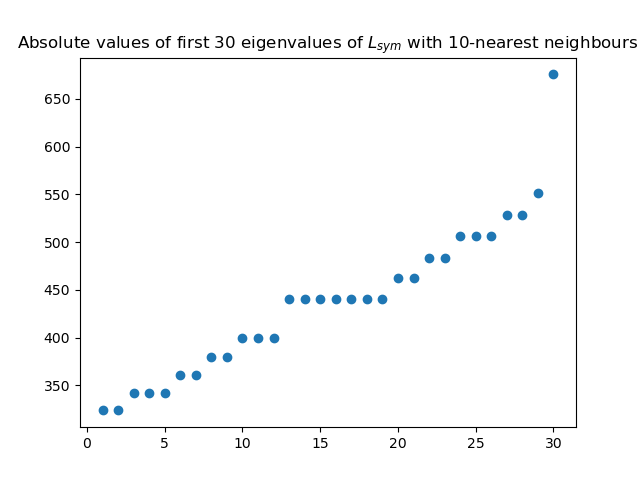
\includegraphics[width=0.5\textheight]{specClustering_l2_k10.png}
			\caption{Ergebnis des spektralen Clusterings unter Verwendung der Euklidischen Distanz und k=10 Nachbarn.}
			\label{fig:result_specClusteringL2}
		\end{center}
	\end{figure}
	\newpage
	\subsection{Standard-Poisoning-Angriffe}
	 Für die Standard-Angriffe mittels des $3 \times 3$ Pixel großen Stickers zeigt sich, dass das \ac{hc} für die korrumpierten Anteile von 5, 10, 15 und 33 Prozent mit einer Genauigkeit von über 99 Prozent funktioniert. Im Gegensatz dazu liegt die Genauigkeit beim \ac{ac} zwischen 57 und 95 Prozent, wobei der Fehler vor allem durch eine relativ schlechte \ac{tnr} zustande kommt. D.h., dass hier trotz vieler Datenpunkte, die richtigerweise als korrumpiert erkannt werden, leider viele saubere Datenpunkte als korrumpiert deklariert werden.
	 
	 \noindent Für einen Anteil von 2 Prozent ist die Detektionsqualität beider Verfahren schlechter als das Clustering auf den Rohdaten und damit unbrauchbar. Die genauen Ergebnisse sind in \autoref{tab:SPA_def_inv3_gwclustering} aufgelistet.
	 \begin{table}[ht]
	 	\begin{center}
	 		\caption[Ergebnisse für Standard-Angriffe]{Qualität der Detektion unterschiedlich starker Angriffe mithilfe des \ac{lrp}-Clusterings und \ac{gwd}. Die Seitenlänge des Stickers beträgt ${s=3}$~Pixel.}
	 		\resizebox{\textwidth}{!}{
	 			
	 			
	 			\begin{tabular}{|c|c|ccc|ccc|}
	 				\hline
	 				Prozentualer 	&   		& 		&	Detektionsrate (\ac{hc}) 		& 		& 		& Detektionsrate (\ac{ac})& 		  \\
	 						
	 				Anteil & 	\ac{aer}		& \ac{acc} 	& 	\ac{tpr} 	& \ac{tnr}  	& \ac{acc} 	& \ac{tpr} 	& \ac{tnr} 	 	\\\hline
	 				
	 				33.00			& 100.00	& \textbf{99.96}	& 99.88		& 100.00& 94.76 & 90.77 & 96.73 \\ 
	 				15.00			& 100.00	& \textbf{100.00}	& 100.00 	& 100.00& 76.51 & 99.31	&72.48 \\
	 				10.00			& 100.00 	& \textbf{99.29 }	& 92.9 		& 100.00& 87.62 & 96.17 & 86.17 \\
	 				5.00			& 100.00		& \textbf{99.48 }	& 90.8		& 99.94 & 57.92 & 20.69 & 59.88  \\
	 				2.00			& 100.00	& 52.85				& 0.0 		& 53.94	& \textbf{52.91} & 0.0 	& 54.0 \\ \hline	 				
	 				
	 				
	 				
	 				
	 		\end{tabular}}
	 		
	 		\label{tab:SPA_def_inv3_gwclustering}	
	 	\end{center}
	 \end{table}
 
	 \noindent Für die Stickergrößen $2\times 2$ und $1\times 1$ ergibt sich ein sehr ähnliches Verhalten, worauf wir im folgenden Abschnitt eingehen werden.
	 
	
	
	
	
		
	


\subsubsection{Variation der Stickergrößen} 
In diesem Abschnitt vergleichen wir die Ergebnisse zusätzlich mit Stickern mit Seitenlänge $s=2$ und $s=1$.

\noindent Auch hier zeigt sich ein ähnliches Verhalten im Vergleich zu $s=3$. Für korrumpierte Anteile über 5 Prozent funktioniert das \ac{hc} deutlich besser. Im Fall $s=1$ werden überraschenderweise auch für einen Anteil von 2 Prozent korrumpierter Daten alle Bilder richtig klassifiziert, d.h. wir erhalten für alle Anteile über 1 Prozent eine Genauigkeit von 100 Prozent. 
\begin{table}[ht!]
	\label{unterschiedlicheStickergrößen}
	\caption{Detektionsraten für Sticker mit Seitenlänge $s=1,2,3$ bei Standard-Angriffen.}
	
	\begin{center}
		\resizebox{\textwidth}{!}{
			
			
			\begin{tabular}{|l|c|c|ccc|ccc|}
				\hline
				Seitenlänge s	& Prozentualer 	&   		& 		&	Detektionsrate \ac{hc}		& 		& 		& Detektionsrate \ac{ac} 	& 	\\	  
				des Auslösers& 	Anteil			& 	\ac{aer}		& \ac{acc} 	& 	\ac{tpr} 	& \ac{tnr}  	& \ac{acc} 	& \ac{tpr} 	& \ac{tnr} 	 	\\\hline
				s=3 			& 33.00			& 100.00	& \textbf{99.96}	& 99.88		& 100.00& 94.76 & 90.77 & 96.73 \\ 
				& 15.00			& 100.00	& \textbf{100.00}	& 100.00 	& 100.00& 76.51 & 99.31	&72.48 \\
				& 10.00			& 100.00 	& \textbf{99.29 }	& 92.9 		& 100.00& 87.62 & 96.17 & 86.17 \\
				& 5.00			& 99.6		& \textbf{99.48 }	& 90.8		& 99.94 & 57.92 & 20.69 & 59.88  \\
				& 2.00			& 100.00	& 52.85				& 0.0 		& 53.94	& \textbf{52.91} & 0.0 	& 54.0 \\ \hline	 				
				s=2 			& 33.00			& 100.00	& \textbf{100.00}& 100.00	& 100.00&99.72	& 99.14	&100.00		\\
				& 15.00			& 100.00	& \textbf{100.00}& 100.00	& 100.00&87.53	& 97.59	& 85.76	\\
				& 10.00			& 100.00	& \textbf{99.72	}& 100.00 	& 99.69	&67.21	& 93.99	& 64.24 \\
				& 5.00 			& 100.00	& \textbf{100.00}& 100.00	& 100.00&47.44	& 10.34	& 49.39 \\
				& 2.00 			& 100.00	& \textbf{58.73	}& 100.00	& 57.88	&49.41	& 17.65	& 50.06	\\
				& 1.00 			& 100.00 	& \textbf{52.37	}& 0.00		& 52.91	& 50.39	& 41.18	& 50.48		 \\\hline
				s=1 			& 33.0 			& 100.0 	& \textbf{100.00}& 100.00	& 100.00& 98.78	& 97.66	& 99.33	 \\ 
				& 15.0			& 100.0		& \textbf{100.00}& 100.00	& 100.00& 96.29	& 79.04	& 99.33	 \\
				& 10.0			& 100.0		& \textbf{100.00}& 100.00	& 100.00& 71.47	& 87.43 & 69.7 	 \\
				& 5.00			& 100.0		& \textbf{100.00}& 100.00	& 100.00& 73.4	& 100.00& 72.0	\\
				& 2.00			& 100.0		& \textbf{100.00}& 100.00	& 100.00& 58.31 & 100.00& 57.45		\\
				& 1.00			& 13.87		& \textbf{60.77 }& 47.06		& 60.91	& 56.99	& 100.00& 56.55 \\ \hline
		\end{tabular}}
	\end{center}
	
\end{table}
	\noindent Durch die Betrachtung dieser Ergebnisse und damit die Beobachtung, dass das \ac{hc} für kleinere Sticker besser funktioniert, führte zu der Vermutung, dass die Detektionsraten auch abhängig von der Position des Stickers und vor allem der Auswahl der zu korrumpierenden Bilder sein könnte. Eine kurze Untersuchung dazu findet sich im folgenden Abschnitt.


	\subsubsection{Vergleich mehrerer Durchläufe für $s=3$}
	Es zeigt sich, dass wir unterschiedliche Ergebnisse für das Clustering erhalten, wenn wir für einen gewissen prozentualen Anteil verschiedene Mengen an zu korrumpierenden Bildern innerhalb einer Klasse auswählen. Um eine etwas allgemeinere Aussage für die Detektion treffen und die Ergebnisse auch spaltenweise miteinander vergleichen zu können, führen wir $n=5$ Angriffe pro prozentualem Anteil durch und bestimmen Mittelwert und Standardabweichung. Dabei unterscheiden sich die Angriffe dahingehend, dass unterschiedliche Bilder an unterschiedlichen Stellen manipuliert werden.
	Die Ergebnisse dazu befinden sich in \autoref{tab:ergebnisse_SPA_s3_gemittelt}.
	
	\begin{table}[H]
		
		\caption{Gemittelte Detektionsraten für Angriffe mit dem Standard-Sticker und $s=3$.}
		\begin{center}
			\resizebox{\textwidth}{!}{
				
				
				\begin{tabular}{|l|c|ccc|ccc|}
					\hline
					Prozentualer	&  				&		&	Detektionsrate (\ac{hc})		& 			& 			& Detektionsrate (\ac{ac})	& 		 \\ Anteil 
					& 			 	& \ac{acc} 	& 	\ac{tpr} 	& \ac{tnr}  		& \ac{acc} 		& \ac{tpr} 	& \ac{tnr} 	 	\\\hline
					
					33.00			& $\varnothing$ 	&\textbf{99.82}	& 99.46	& 100.00	& 90.36		& 94.41& 87.16   \\ 
					& $\sigma$		& 0.19	& 0.58 	& 0.00	& 6.81 		& 2.98		& 9.96 \\ \hline
					15.00			& $\varnothing$	&\textbf{99.89}	& 99.32	& 99.98	& 85.24		& 96.56& 83.24   \\ 
					& $\sigma$		& 0.17	& 1.17 	& 0.024	& 10.75 	& 1.98	& 12.88 \\ \hline
					10.00			& $\varnothing$	& \textbf{97.85}	& 95.93 	& 99.94& 68,82		& 77.92	& 67.82   \\ 
					& $\sigma$		& 3.81	& 2.61 	& 0.09 & 17.82 		& 35.90	& 17.17 \\ \hline
					5.00 			& $\varnothing$	& \textbf{89.42}	& 87.43	& 89.48 & 57.77 & 36.55 & 58.88 \\
									&$ \sigma$& 13.15& 23.99 & 13.01 & 3.73 & 40.01 & 2.42 \\ \hline
					2.00 			& $\varnothing$	& \textbf{56.42}	& 80.00	& 55.89 & 52.48 & 24.118 & 53.07 \\
									&$ \sigma$& 4.30&  40.00& 4.04 & 2.12 & 38.28 & 2.42 \\ \hline
			\end{tabular}}
			\label{tab:ergebnisse_SPA_s3_gemittelt}
		\end{center}
	
	\end{table}

	\noindent \autoref{tab:ergebnisse_SPA_s3_gemittelt} zeigt Mittelwert und Standardabweichung für \ac{acc}, \ac{tpr} und \ac{tnr} für Angriffe mit verschiedenen Anteilen an korrumpierten Daten. Beim \ac{hc} wird deutlich, dass die Standardabweichung für kleiner werdende Anteile zunimmt. Beim Vergleich beider Detektionsverfahren zeigt sich, dass die Abweichung für das \ac{ac} deutlich über der des \ac{hc} liegt.

	\subsection{Label-konsistente Poisoning-Angriffe}
	\begin{comment}
	
	
	\begin{remark}
		Für einen einzelnen Amplitudensticker mit d=10 ist das eigentlich identisch zu dem Angriff mit dem Sticker
	\end{remark}

	
	\begin{figure}[h]
		\begin{center}
			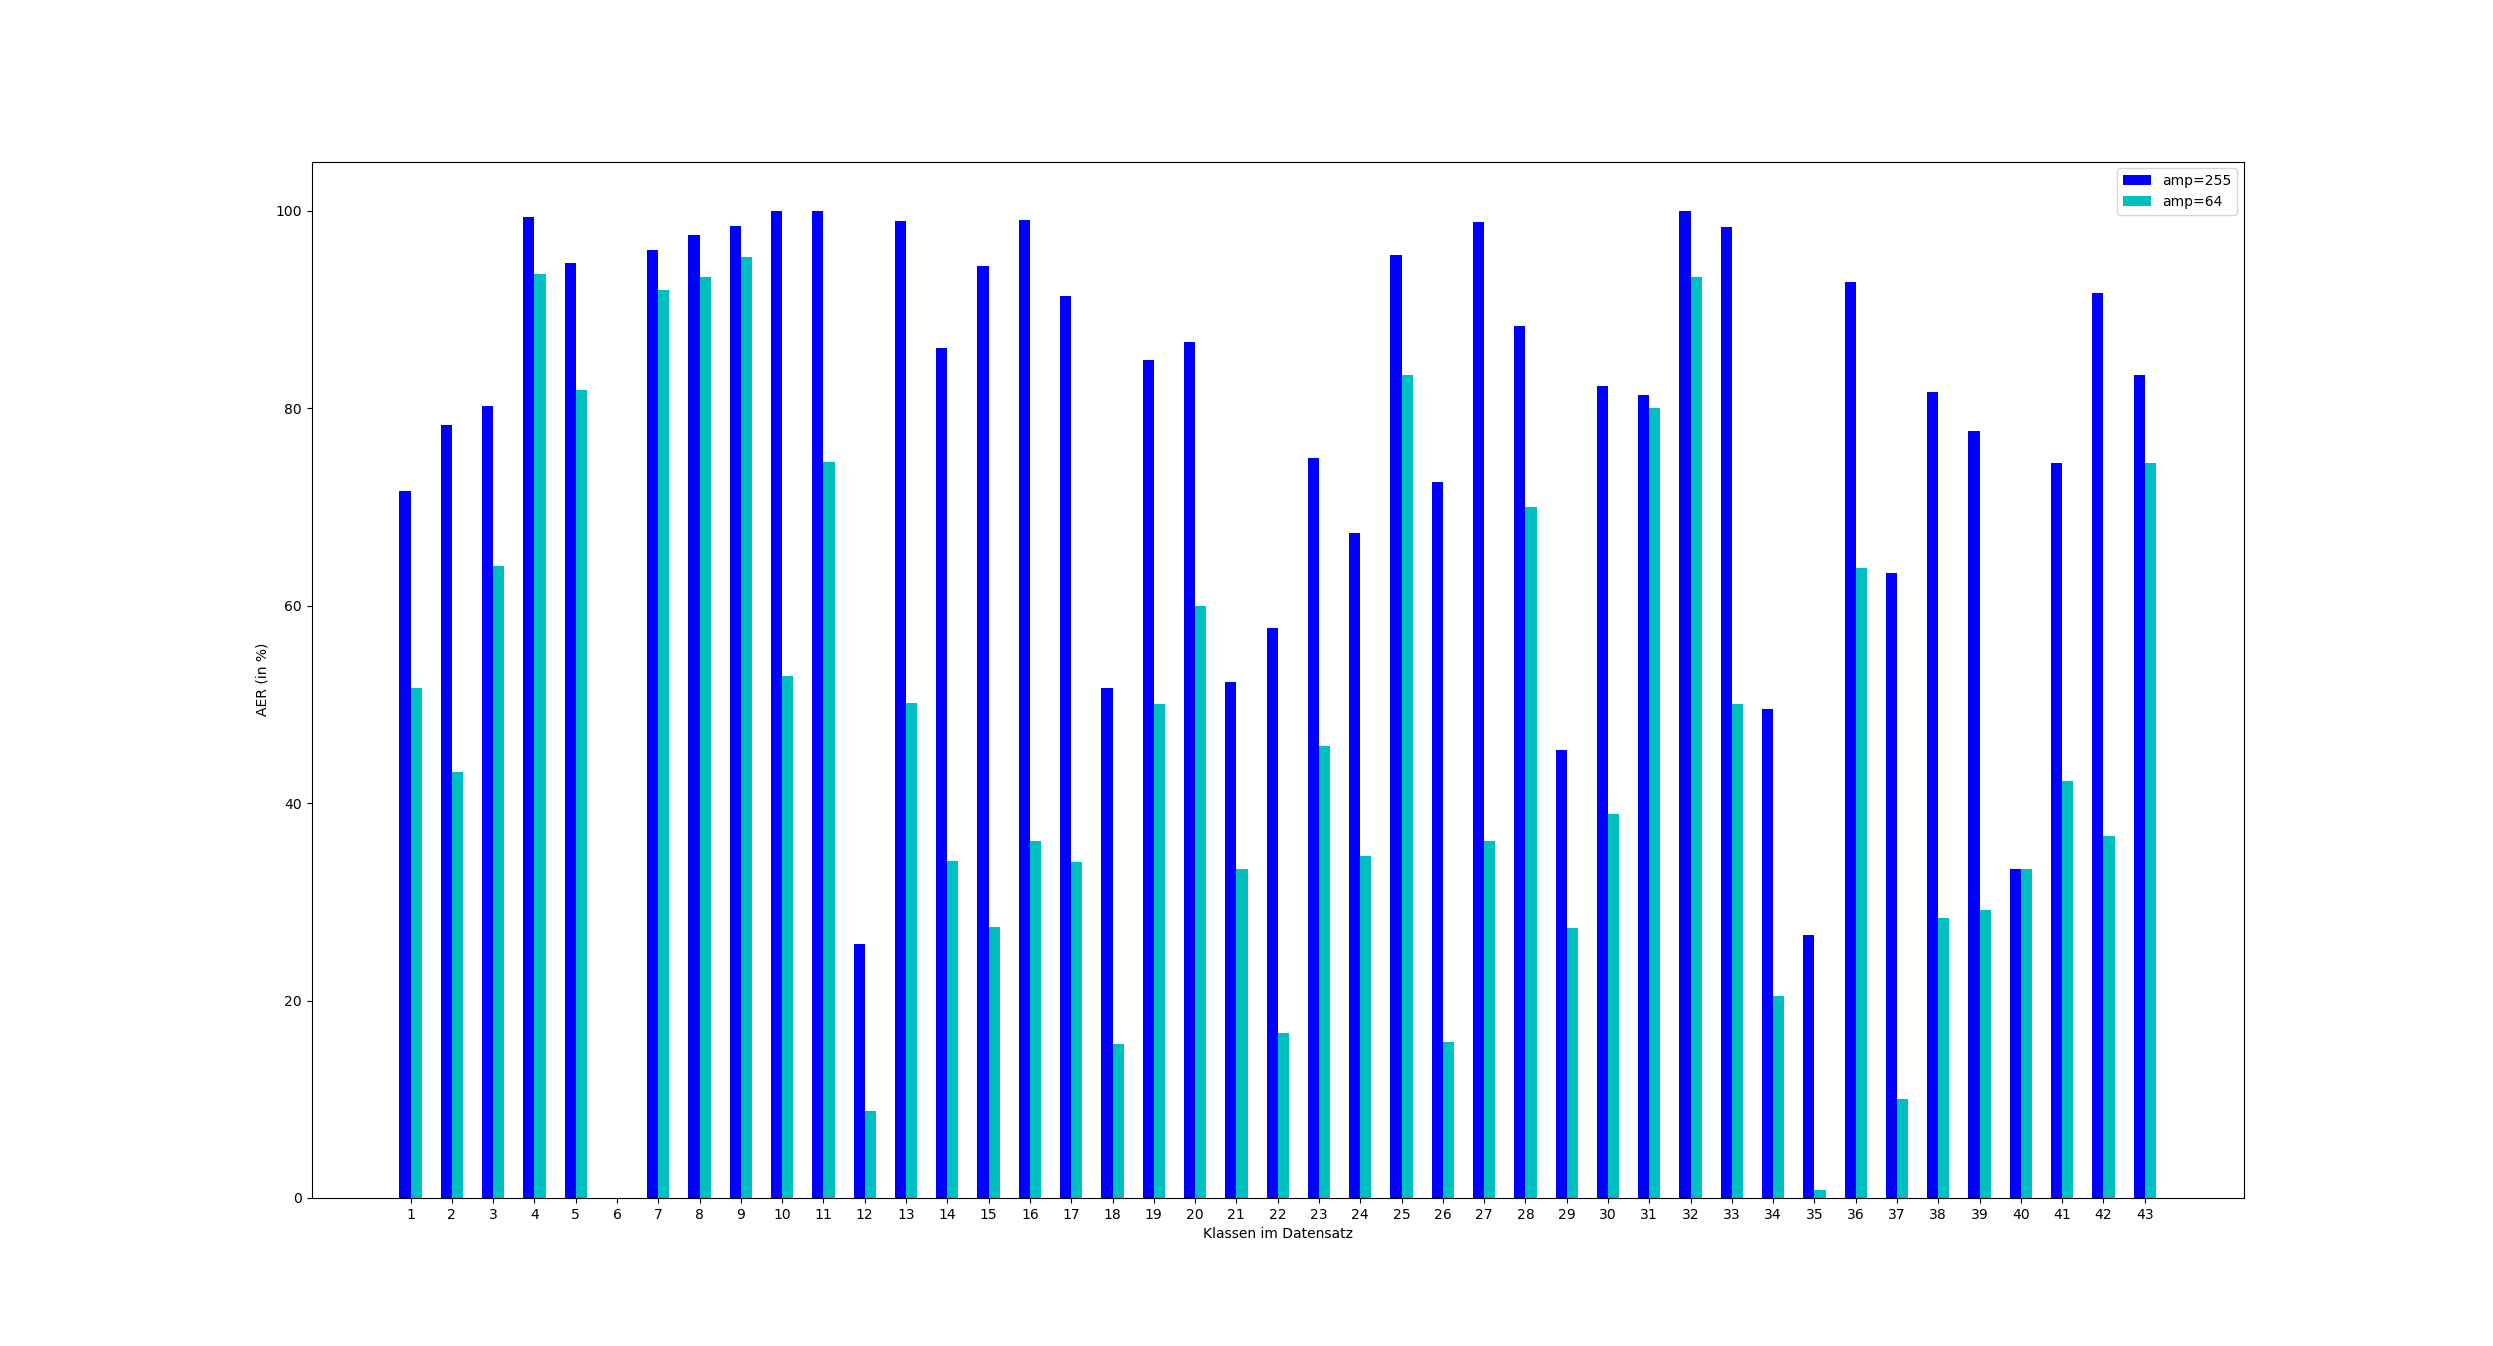
\includegraphics[width=0.75\textheight]{Vergleich_AER_CLPA.png}
			\caption{Angriffserfolgsrate pro Klasse bei Clean-Label-Poisoning-Attacks für verschiedene Werte \textit{amp} des Amplitudenstickers in vierfacher Ausführung bei Abstand $d=10$ zum Rand}
			\label{fig:AER_proKlasse_CLPA}
		\end{center}
	\end{figure}
	
	In \autoref{fig:AER_proKlasse_CLPA} sind die Angriffserfolgsraten pro Klasse im Fall von $33 \%$ korrumpierten Daten und dem Amplitudensticker in jeder der 4 Bildecken mit dem Abstand von 10 Pixeln zum Rand dargestellt. In beiden Fällen geben wir keine AER für die Klasse 6 an, über die der Angriff stattfindet.
	Die mittlere Angriffserfolgsrate beträgt für $amp=255$ $79.15 \%$. In mehreren Klassen wird eine AER von $100 \%$ erreicht.\\
	Für $amp=64$ fällt der Angriff mit einer mAER von $48.17 \%$ deutlich schwächer aus. Die maximal erreichte AER beträgt $95.33 \%$ in Klasse 10. Die minimalen AER sind $25 \%$ bzw. $0.83 \% $.
	Eine weitere Reduktion der Amplitude auf $amp=32$ führt zu einer mAER von $6.55 \%$ und einer maximalen AER von $33 \%$.
	
	Für d=0, amplitude=64 und eps=1200 ergibt sich kein erfolgreicher Angriff, dabei war fast alles 0, die Trigger im Testdatensatz waren auch auf 64
	Jetzt für d=10, auch hier gilt amp=64 im Testdatensatz:Ergebnis:
	
	

	
	%\subsection{Auswertung der CLPA}
	\end{comment}
	In diesem Abschnitt vergleichen wir die Detektion der \acp{lkpa}. Wir verwenden dabei den grün-gelben $3\times 3$ großen Sticker, der nach einer Störung des Ausgangsbildes eingefügt wird.
	Hervorzuheben ist hierbei, dass die \ac{maer} für alle prozentualen Anteile recht hoch ist. Für die Anteile 33, 15, 10 und 5 Prozent funktioniert die Detektion bei beiden Verfahren im Bezug auf die \ac{acc} ähnlich gut, wobei die \ac{tpr} beim \ac{hc} um bis zu 12 Prozentpunkte höher liegt.\\
	\noindent Für einen Anteil von 2 Prozent korrumpierten Daten funktioniert der Angriff mit einer \ac{maer} von 83.51 Prozent ähnlich gut wie die Angriffe mit höheren korrumpierten Anteilen, beide Detektionsverfahren erweisen sich für diesen Fall jedoch als nutzlos. Die Ergebnisse sind in \autoref{tab:Ergebnisse_CLPA} dargestellt.
	
	
	\begin{table}[ht]
		\caption[Ergebnisse der Detektion von Label-konsistenten Poisoning-Angriffen mit gelb-grünen Stickern]{Ergebnisse der Detektion von Label-konistenten Poisoning-Angriffen mit gelb-grünen Stickern bei verschiedenen Anteilen korrumpierter Daten für \ac{hc} und \ac{ac}.}
		\begin{center}
			\resizebox{\textwidth}{!}{
				\begin{tabular}[h]{|l|c|ccc|ccc|} \hline
					Prozentualer&		&		& Detektionsrate (\ac{hc})	& 		& 		&Detektionsrate (\ac{ac})&		\\ 
					Anteil 	& \ac{maer} 	& \ac{acc} 	& \ac{tpr} 					& \ac{tnr} 	& \ac{acc} 	& \ac{tpr} 				& \ac{tnr} 	\\ \hline
					
					33 		& 90.98	& \textbf{99.58}	& 98.71					&100.0	& 99.09 & 97.24 			& 100.0 \\
					15		& 83.15 & \textbf{98.91} & 96.69  				&100.0	& 96.42 & 89.15				& 100.0 \\
					10		& 90.45 & \textbf{99.82} & 98.18					&100.00 & 98.97 & 89.7				& 100.0 \\
					5		& 84.77 & \textbf{99.82} & 96.34					&100.00	& 99.09 & 84.15				& 99.87 \\
					2		& 83.51 & 55.33 & 100.00				& 54.42	& \textbf{56.3}	& 100.00 			& 55.41 \\ \hline
				\end{tabular}	
				
				
			}
		\end{center}
		
		\label{tab:Ergebnisse_CLPA}
		
	\end{table}

	\noindent Bei 10 Prozent korrumpierten Daten erkennt das \ac{hc} nur 3 anstatt 17 Punkten als falsch-negativ. Bei 5 Prozent treten nur 3 anstatt 13 Falsch-Negative auf.

	
	\subsection{Detektion bei reduzierten Amplitudenstickern}
	In diesem Abschnitt werten wir die Ergebnisse der Detektion von \acp{lkpa} bei weniger sichtbaren Auslösern in Form eines Amplitudenstickers mit reduzierter Amplitude aus.\\
	
	\noindent Die Angriffe wurden für die Amplituden $amp=32,64,128$ ausgeführt. Wir können dafür eine \ac{aer} pro Klasse angeben, siehe dazu \autoref{fig:AER_proKlasse_CLPA_amp}. Dabei ist zu beachten, dass wir keine \ac{aer} für die Klasse 5 (80 km/h) angeben, die als Zielklasse ausgewählt wurde. Hier wird deutlich, dass die \ac{aer} bei ${amp = 128}$ in allen Klassen nahezu bei 100 Prozent liegt. Sowohl für ${amp = 64}$ als auch $amp=32$ sind die \ac{aer} für die ersten 10 Klasse größer als für die restlichen. Unter der Verwendung der Sticker mit der Amplitude $amp=32$ existieren auch einige Klassen, bei denen die \ac{aer} beinahe 0~Prozent beträgt.
	
	\begin{figure}[!h]
		\begin{center}
			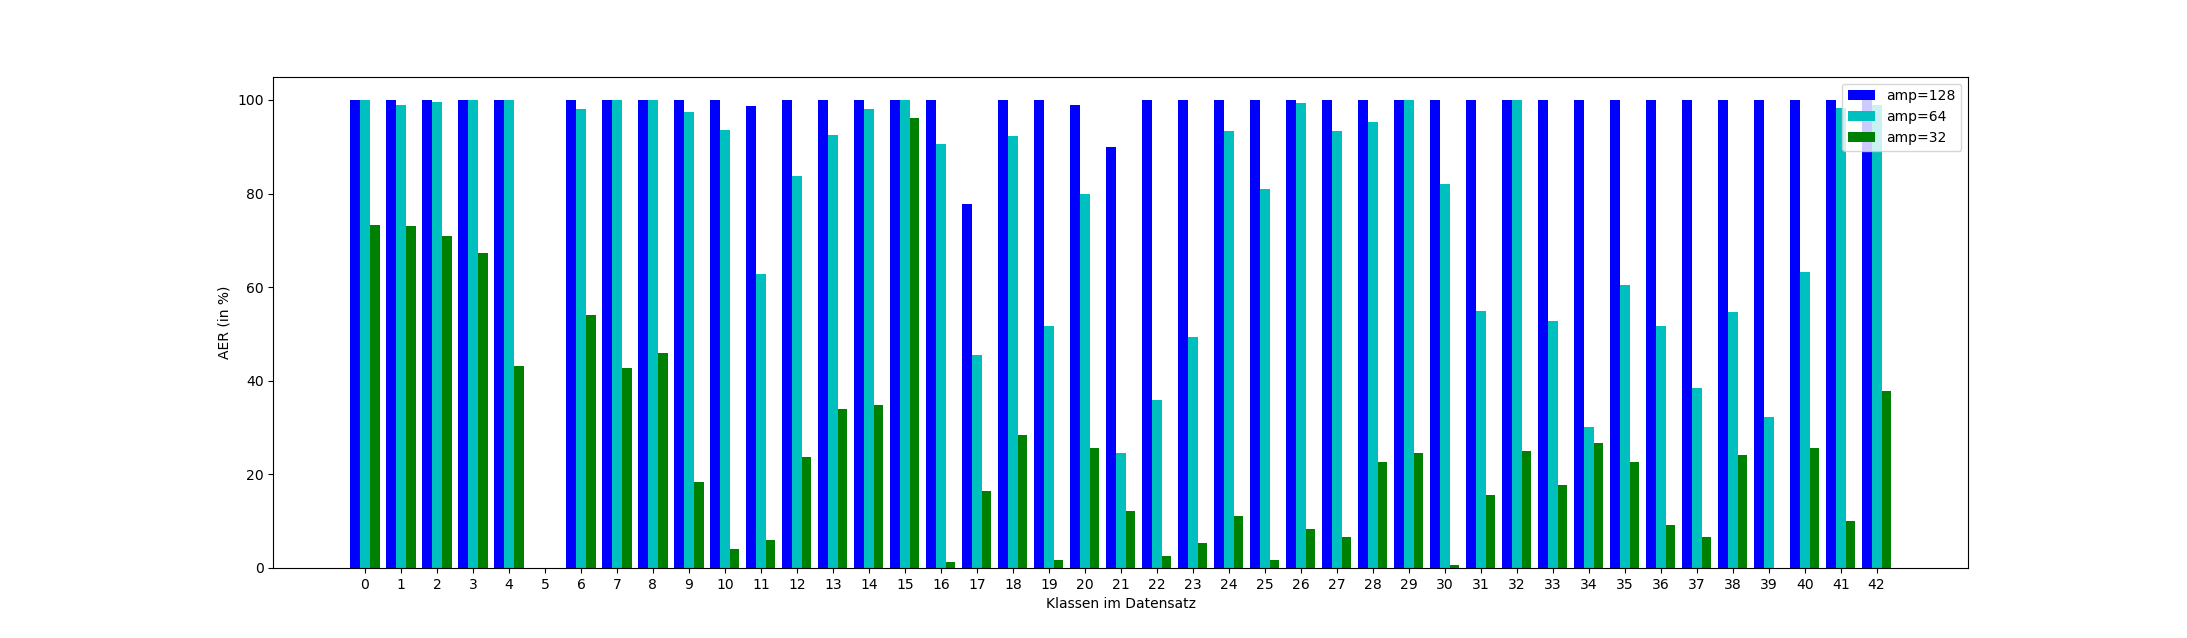
\includegraphics[width=\textwidth]{vergleich_CLPA_AER_amp.png}
			\caption[\ac{aer} pro Klasse bei LkPAs]{\ac{aer} pro Klasse bei \ac{lkpa} bei einem Amplitudensticker mit Abstand $d=10$ zur rechten unteren Ecke. Die \ac{aer} sind pro Klasse für die Amplitudenwerte $amp=128,64,32$ aufgetragen.}
			\label{fig:AER_proKlasse_CLPA_amp}
		\end{center}
	\end{figure}
	
	\noindent In \autoref{tab:Ergebnisse_CLPA_reduced} sind die Ergebnisse der jeweiligen Angriffe für die Detektion mit \ac{hc} und \ac{ac} gegeben. Wir sehen, dass die \ac{maer} mit der Reduktion der Amplitudenstärke deutlich abnimmt. Während die Detektionsrate für beide Verfahren bei $amp=128$ bei über 99 Prozent liegt, nimmt die Detektionsqualität mit abnehmender \ac{maer} ebenfalls deutlich ab. Für den Fall $amp=32$ mit einer \ac{maer} liegt die \ac{acc} für beide Verfahren noch immer bei etwa 80~Prozent. Dabei ist die \ac{tnr} in beiden Fällen höher als die \ac{tpr}. \\
	
	\begin{table}[!h]
		\caption{Ergebnisse der Detektion von LkPAs mit reduzierten Amplitudenstickern bei einem Anteil korrumpierter Daten von 33 Prozent.}
		\begin{center}
			\resizebox{\textwidth}{!}{
				\begin{tabular}[h]{|c|c|ccc|ccc|}\hline
				&		&		& Detektionsrate (HC)	& 		& 		&Detektionsrate (AC)&		\\
				Amplitudenstärke 	& mAER 	& ACC 	& TPR 					& TNR 	& ACC 	& TPR 				& TNR 	\\ \hline
				
				128 				& 99.18	& \textbf{99.7}	& 99.08					&100.0	& 99.45 & 98.35 			& 100.0 \\
				64					& 77.97 & 90.79 & 74.08 				&99.01	& \textbf{92.06} & 90.44				& 92.86 \\
				32					& 25.65 & \textbf{81.58} & 58.46					& 92.95 & 78.97 & 74.26				& 81.28 \\ \hline
				
			\end{tabular}	
				
				
			}
		\end{center}
	
		\label{tab:Ergebnisse_CLPA_reduced}
		
	\end{table}



\noindent Der Unterschied beim Clustering im Fall $amp=128$ besteht darin, dass das \ac{hc} nur 5 anstatt 9 Datenpunkten als falsch-negativ klassifiziert.
	
	
\noindent Vergleichen wir die Ausgaben der \ac{lrp} für die Werte ${amp=64}$ und ${amp=32}$, wird deutlich, dass die \ac{lrp} den Sticker nicht mehr als die relevante Größe im Bild erkennt. Die Vermutung liegt nahe, dass dies also an der \ac{lrp} liegen muss. Es ist jedoch so, dass das \ac{nn} im Fall $amp=32$ bereits ein Viertel aller Auslöser nicht mehr erkennt. Ein Vergleich zweier Heatmaps findet sich in \autoref{fig:vergleich_heatmaps_red_Amplituden}.
	
	\begin{figure}
		\centering
		\begin{subfigure}{.5\textwidth}
			\centering
			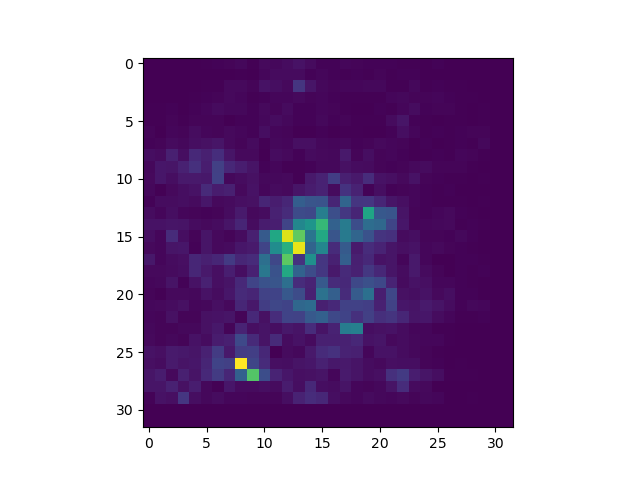
\includegraphics[width=.7\linewidth]{140_poison_CLPA_1sticker_amp32n5d10e-rule_heatmap.png}
			%\caption{Verkehrsschild der Klasse 'Höchstgeschwindigkeit: 50km/h' versehen mit einem 3x3 Sticker und dem Label 'Höchstgeschwindigkeit: 80km/h'}
			
		\end{subfigure}%
		\begin{subfigure}{.5\textwidth}
			\centering
			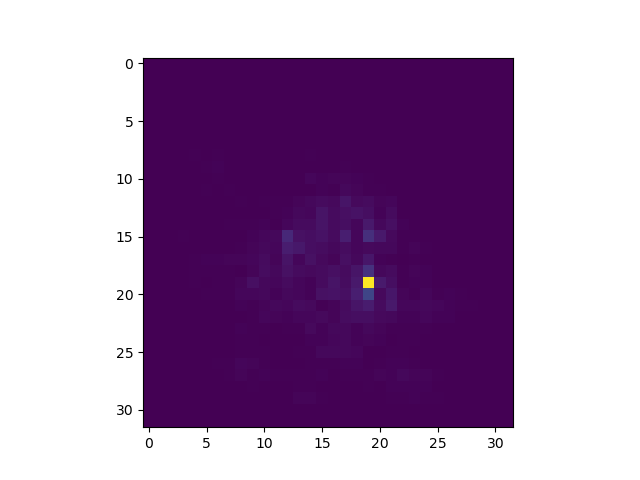
\includegraphics[width=.7\linewidth]{140_poison_CLPA_1sticker_amp64n5d10e-rule_heatmap.png}
			%\caption{Zugehörige Heatmap bezüglich der Klasse 'Höchstgeschwindigkeit: 80km/h'}
			
		\end{subfigure}
		\caption[Vergleich zweier Heatmaps mit Amplitudenstickern.]{\textbf{Links:} Heatmap eines korrumpierten Bildes bei der Verwendung eines Amplitudenstickers mit $amp=32$.  \textbf{Rechts:} Heatmap eines korrumpierten Bildes bei der Verwendung eines Amplitudenstickers mit $amp=64$.}
		
		
		\label{fig:vergleich_heatmaps_red_Amplituden}
	\end{figure}
	

	\section{Einordnung der Ergebnisse}
	%Getroffene Annahmen
	Für die Standard-Angriffe zeigt sich, dass bereits für sehr kleine Anteile an korrumpierten Daten ein erfolgreicher Angriff möglich ist.
	Wir vermuten, dass sich größere \acp{nn} leichter manipulieren lassen, da sich dort bereits mit weniger korrumpierten Daten eine Hintertür erfolgreich implementieren lässt. \\
	
	\noindent Für die Detektionsverfahren im Fall des Standard-Angriffs konnten wir sehen, dass das \ac{hc} für die Seitenlänge des Stickers $s=3$ für alle prozentualen Anteile eine bessere Genauigkeit als das \ac{ac} aufweist, das als vorheriger State-of-the-Art angesehen werden kann. Es wird deutlich, dass dies vor allem dadurch zustande kommt, dass die \ac{tnr} bei nahezu 100 Prozent liegt. Auch die \ac{tpr} liegt für Anteile bis zu 5 Prozent korrumpierter Daten über 90~Prozent, während das Activation-Clustering bei 5 Prozent nicht mehr funktioniert.
	
	\noindent Bei \acp{lkpa} unter Verwendung des $3\times 3$ Pixel großen Stickers zeigt sich, dass wir mit dem \ac{hc} ein Verfahren besitzen, das diese Angriffe detektieren kann. Im entsprechenden Paper \cite{labelconsistent} wurde davon ausgegangen, dass kein solches Verfahren existiert. Überraschenderweise funktioniert auch das \ac{ac} hier relativ gut.
	
	\noindent Für den Fall von \acp{lkpa} mit reduzierten Amplitudenstickern funktioniert die Detektion deutlich schlechter. Dies liegt auch daran, dass sich die Angriffe schwieriger umsetzen lassen. Wir konnten den korrumpierten Anteil von 33 Prozent nicht weiter absenken, sodass gleichzeitig ein erfolgreicher Angriff entstand. In \cite{labelconsistent} gelten beispielsweise Angriffe mit einer \ac{aer}, die in jeder Klasse größer als 50 Prozent ist, als erfolgreich. Solche Angriffe zu detektieren, ist auch mit den vorgestellten Verfahren leider nicht möglich. Die Schwierigkeit liegt darin, dass das \ac{nn} den Auslöser bereits so schlecht lernt, dass auch die erzeugten Heatmaps diese nicht wiedergeben können. Wichtig ist jedoch, dass dies dann nicht auf die \ac{lrp} zurückzuführen ist, sondern auf den Angriff und das \ac{nn} selbst. 	
	\noindent Es ist zu beachten, dass die Laufzeit für das Activation-Clustering deutlich unter der Laufzeit des Heatmap-Clusterings liegt. Die beiden wichtigsten Schritte bilden die Berechnung der \ac{lrp}-Heatmap und das Clustering. Der für die Berechnung deutlich aufwendigere Teil entfällt auf das Clustering selbst, bei dem die \ac{gwd} wiederholt berechnet werden muss. Durch die Verwendung der entropisch-regularisierten \ac{gwd} wird dies soweit beschleunigt, dass sie nur einen Bruchteil der Trainingszeit des verwendeten \ac{nn} benötigt.
	
	
	
		
	
	\newpage 
	
	
	\chapter{Zusammenfassung und Ausblick} \label{chapter_conclusion}
	In dieser Arbeit haben wir, basierend auf \cite{unmaskingCH}, ein neues Verfahren zur Detektion von \acp{pa} vorgestellt und mit dem \ac{ac} verglichen.
	
	\noindent Wir konnten sehen, wie sich das \ac{hc} im Vergleich zum \ac{ac} als Detektionsverfahren für verschiedene Poisoning-Angriffe (Standard-Backdoor-Poisoning-Angriffe, Label-konsistente Poisoning-Angriffe und Label-kon\-sis\-ten\-te Poi\-so\-ning-Angriffe mit reduzierter Sichtbarkeit des Auslösers) verhält.
	
	\noindent Es zeigte sich, dass die von uns ausgeführten Angriffe mithilfe des \ac{hc} im Vergleich zum \ac{ac} besser detektiert werden können.
	\noindent Die Vermutung, dass das \ac{ac} sehr schlecht funktioniert, bestätigte sich nicht. In \cite{labelconsistent} wird angegeben, dass zu dieser Art von Angriff bisher keine Detektionsverfahren bekannt wären. Sowohl das \ac{ac} als auch das \ac{hc} konnten diese Angriffe jedoch für korrumpierte Anteile über 2 Prozent erfolgreich aufdecken.
	
	\noindent Die \ac{lrp} wird bisher nicht in großem Maßstab in der Praxis eingesetzt. Die Schwierigkeit der Implementierung des \ac{hc} liegt darin, \ac{lrp}-Heatmaps für verschiedene Netzarchitekturen zu erzeugen.
	
	\noindent In vorherigen Untersuchungen konnten wir feststellen, dass Poisoning-Angriffe für größere \acp{nn} deutlich besser funktionieren. Auch in \cite{labelconsistent} wurde beispielsweise ein ResNet \cite{resnet} oder VGG-16 \cite{vgg16} verwendet.
	Während sich Angriffe auch für kleine Anteile an korrumpierten Daten implementieren lassen, wird das Clustering sowohl für \ac{ac} als auch \ac{hc} in diesem Fall sehr schwierig.
	
	\noindent Besonders interessant sind die Angriffe, die eine \ac{aer} von (deutlich) weniger als 100 Prozent aufweisen. Diese werden nur schlecht von beiden Verfahren erkannt und stellen somit aus Sicht des Angreifers den optimalen Angriff dar. Mit einem Angriff, der nur eine \ac{aer} von etwa 50 Prozent aufweist, hätte ein Angreifer einen Angriff konstruiert, der häufig funktioniert, jedoch nicht von einem der vorgestellten Verfahren detektiert werden könnte.\\
	
	\noindent In weiteren Untersuchungen sollten Angriffe auf weitere Datensätze wie beispielsweise LISA, MNIST oder CIFAR-10 durchgeführt werden. Vor allem für die Implementierung der Label-konsistenten Angriffe wäre ein Vergleich auf größeren \acp{nn} interessant.
	
	\noindent Möglich wäre auch die Kombination verschiedener \ac{lrp}-Regeln (Composite-\ac{lrp}) oder der Softmax Gradient \ac{lrp} \cite{sglrp}.
	
	\noindent In \cite{toxic} werden Benchmarks für alle bekannten Arten von \acp{pa} vorgestellt, um zukünftige Arbeiten im Bereich von \acp{pa} auf einer gemeinsamen Grundlageff vergleichen zu können. Interessant wäre dabei, wie sich das \ac{hc} für die dort vorgestellten Angriffe verhält. Dabei werden ebenfalls deutlich größere Datensätze und \acp{nn} verwendet.
	
	\noindent In \cite{findingandremoving} wird ein Vorgehen präsentiert, das die Laufzeit des \ac{hc} deutlich reduziert. Dort werden nicht nur die Heatmaps in der Eingabeschicht verwendet, sondern die Repräsentation besteht aus Heatmaps von speziell ausgewählten Zwischenschichten, die bezüglich einer $L^p$-Distanz anstatt der sehr rechenintensiven \ac{gwd} miteinander verglichen werden. 
	
	
	\bibliographystyle{alpha}
	
	\bibliography{bibfileMAlukasschulth}
	
	
	
\end{document}
